\renewcommand{\thefigure}{A.\arabic{figure}}
\setcounter{figure}{0}

\section*{Annexes}

\begin{figure}[H]
	\begin{center}
		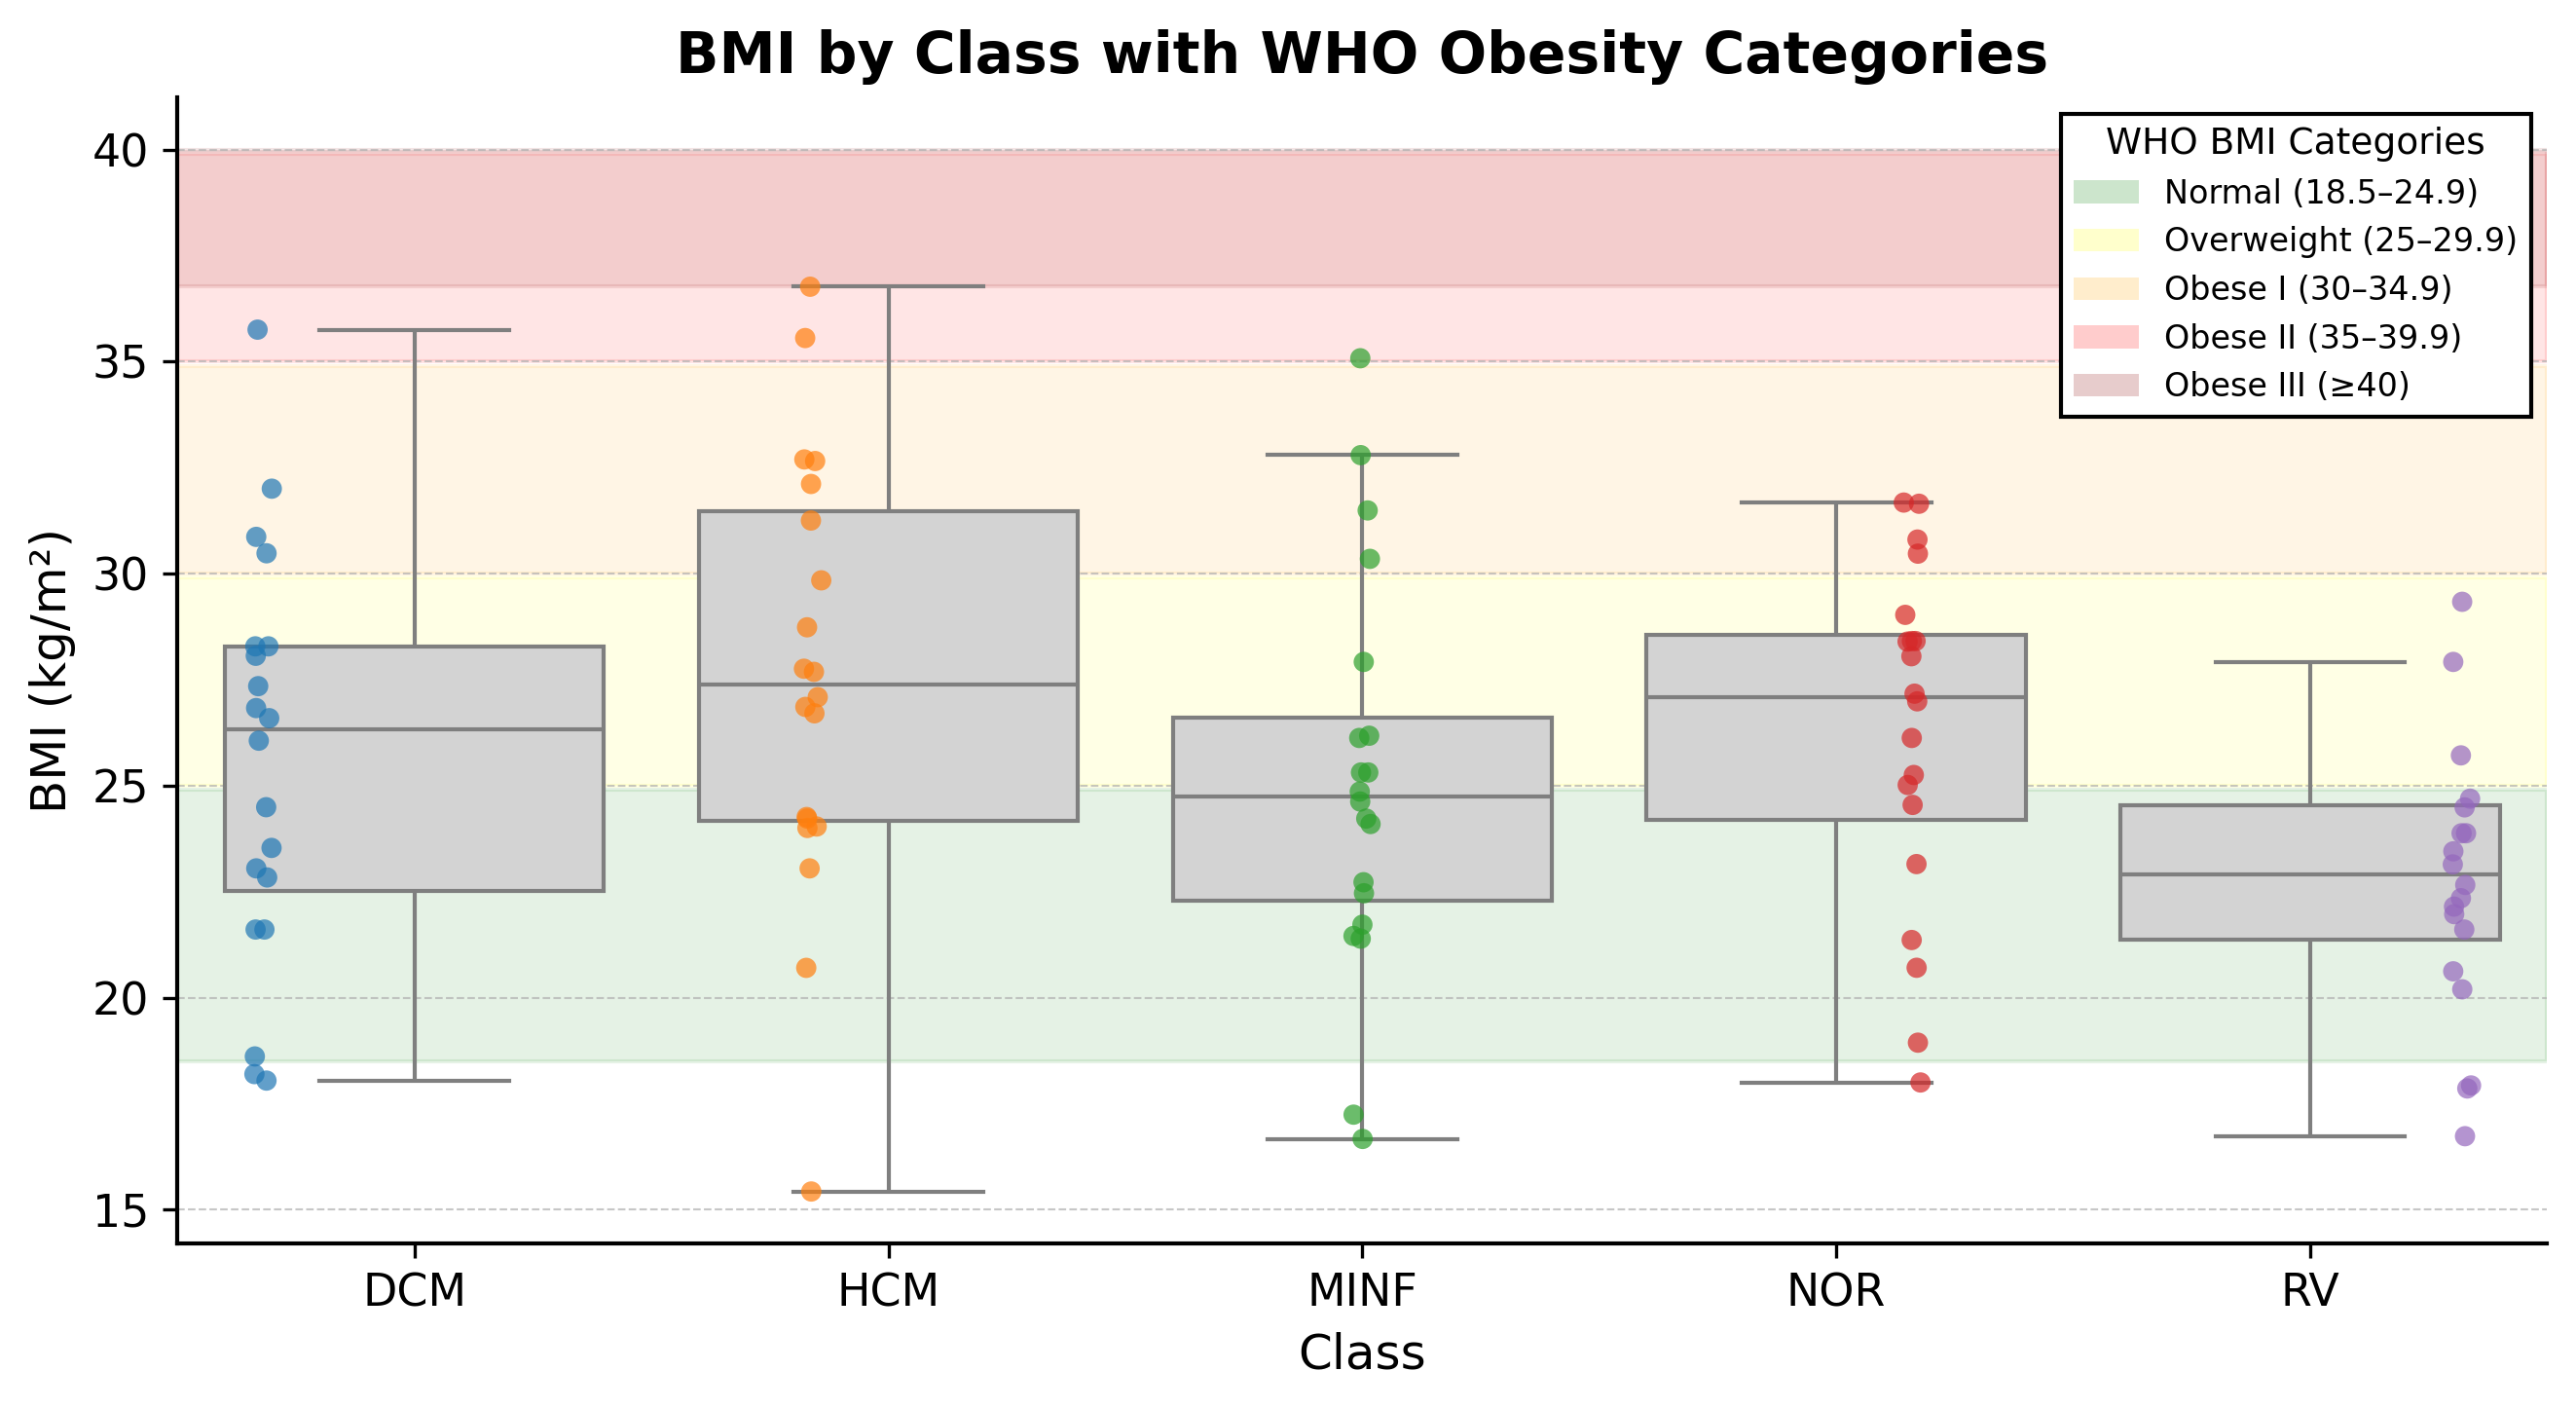
\includegraphics[width=0.99\textwidth]{../images/eda/bmi_by_class.png}
	\end{center}
	\caption{Distributions of Body Mass Index (BMI, kg/m\textsuperscript{2})
		across classes. DCM $=$ Dilated Cardiomyopathy, HCM $=$ Hypertrophic
		Cardiomyopathy, MINF $=$ Myocardial Infarction, NOR $=$ Normal, RV $=$ Right
		Ventricular abnormality.}
	\label{fig:figA1}
\end{figure}

\hfill

\begin{figure}[H]
	\begin{center}
		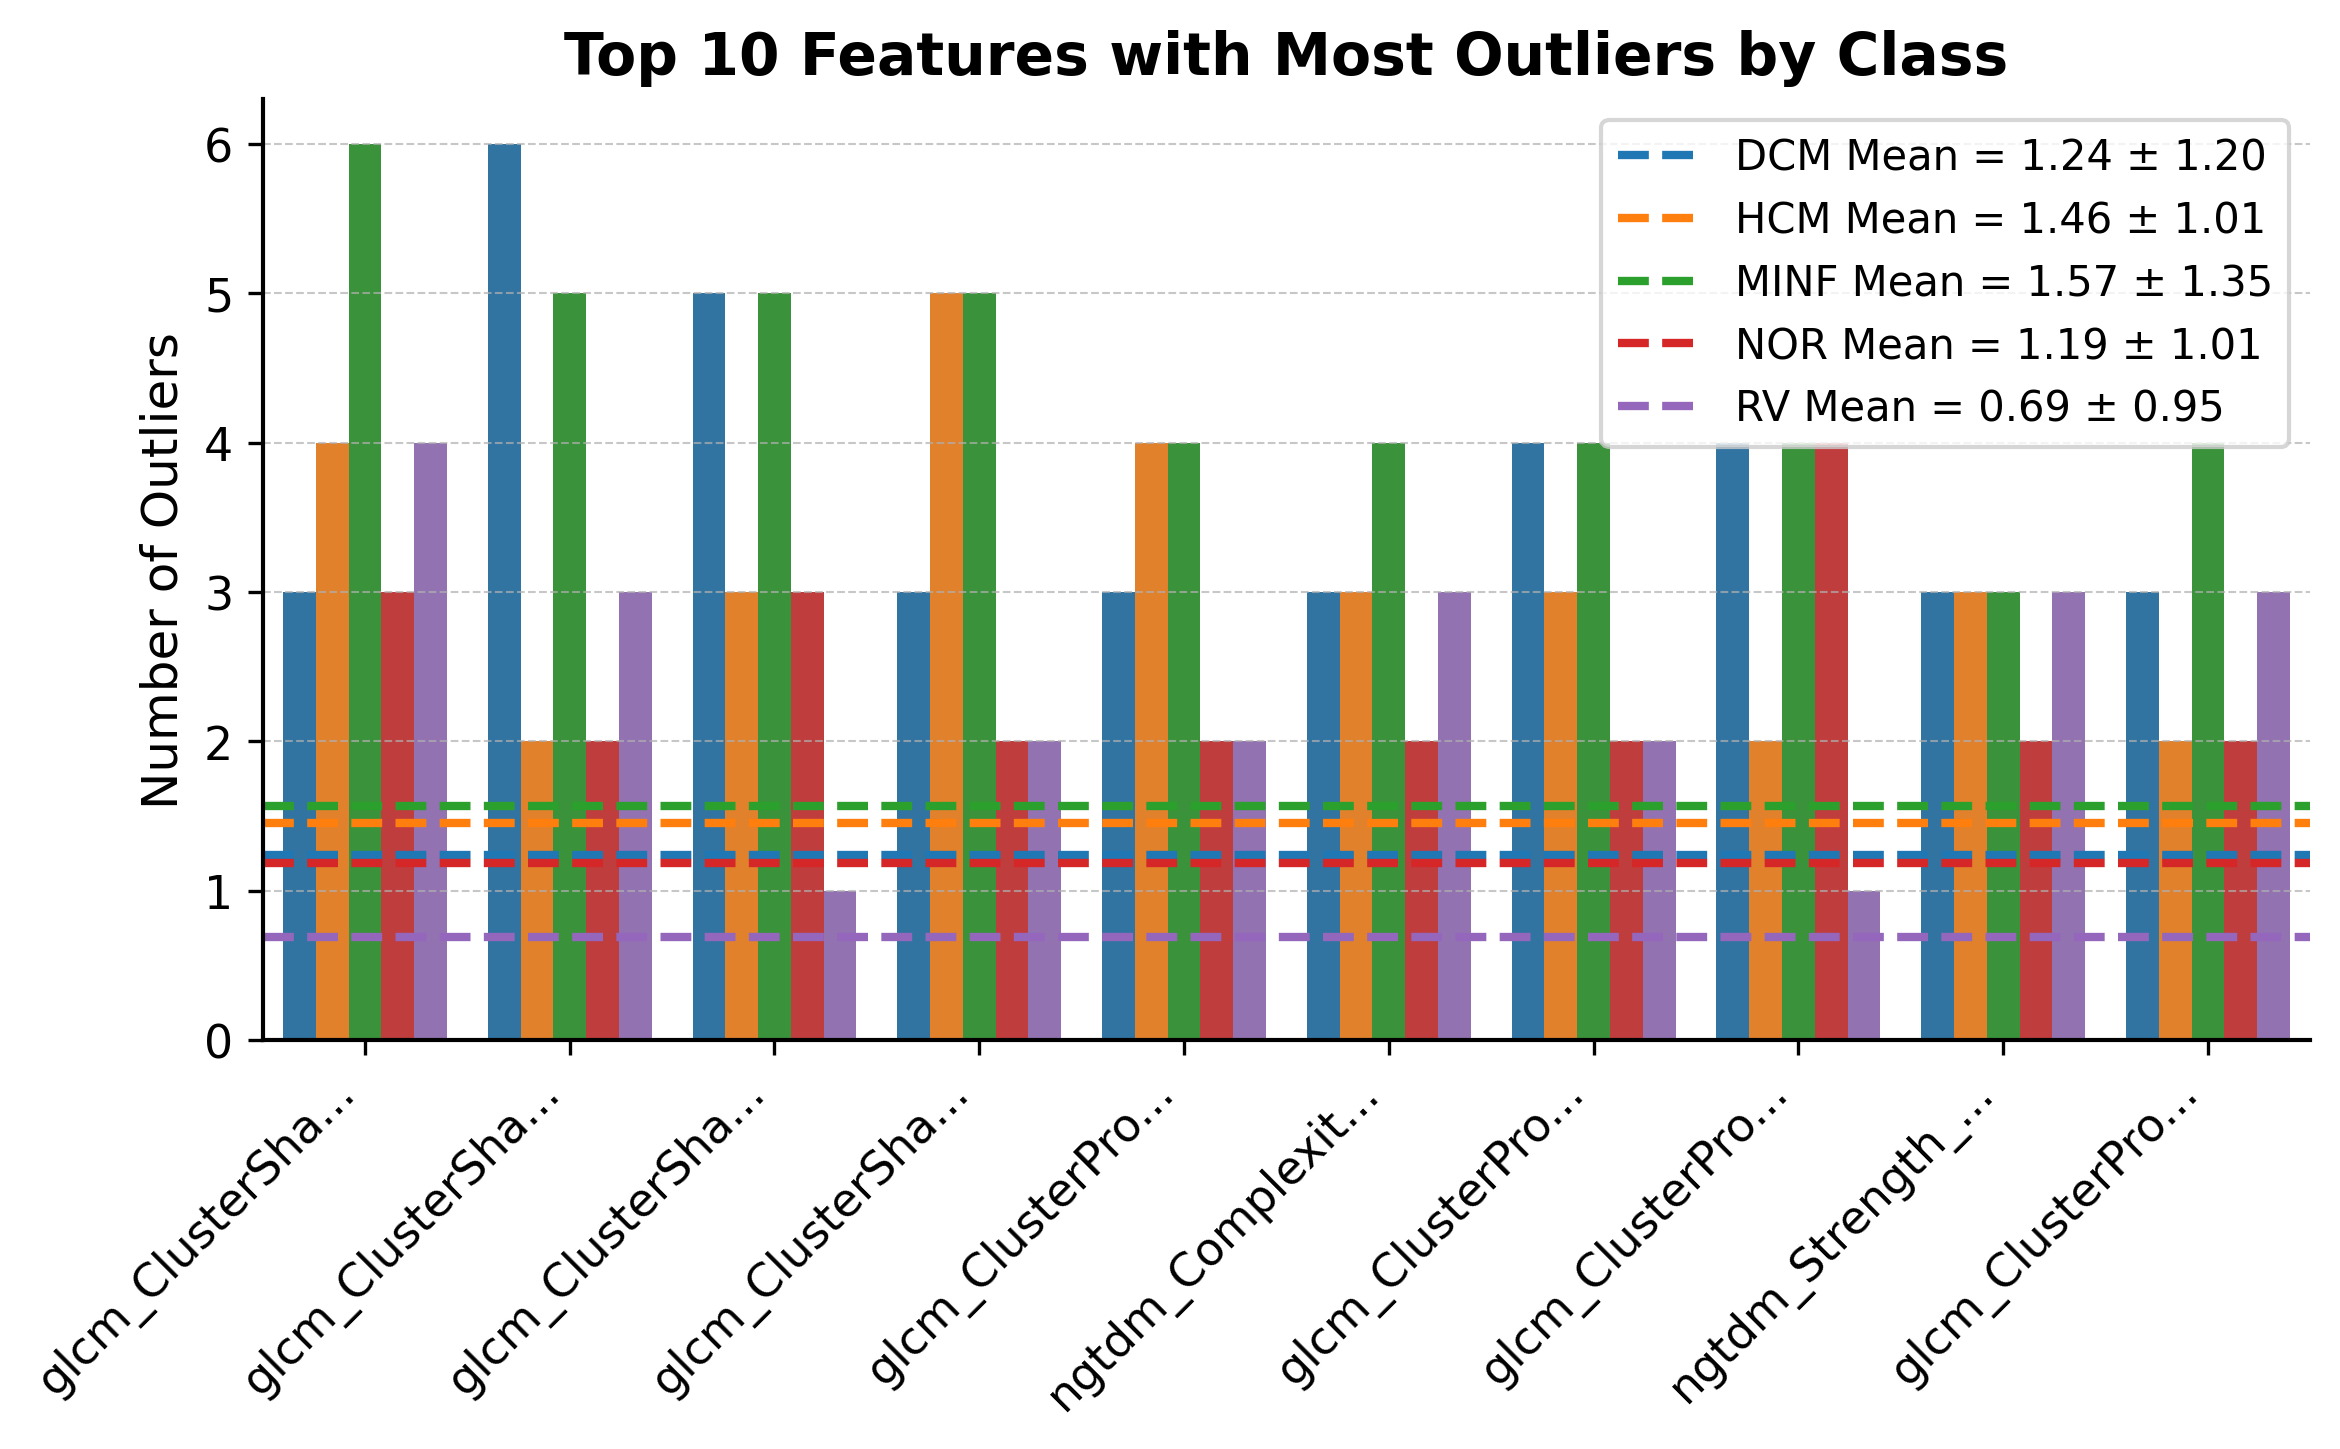
\includegraphics[width=0.99\textwidth]{../images/eda/outliers.png}
	\end{center}
	\caption{Top 10 features with the highest total number of outliers. Bars are
		grouped by class and represent the number of outliers per feature-class pair.
		The red dashed line marks the overall mean ± standard deviation.}
	\label{fig:figA2}
\end{figure}


\begin{figure}
	\begin{center}
		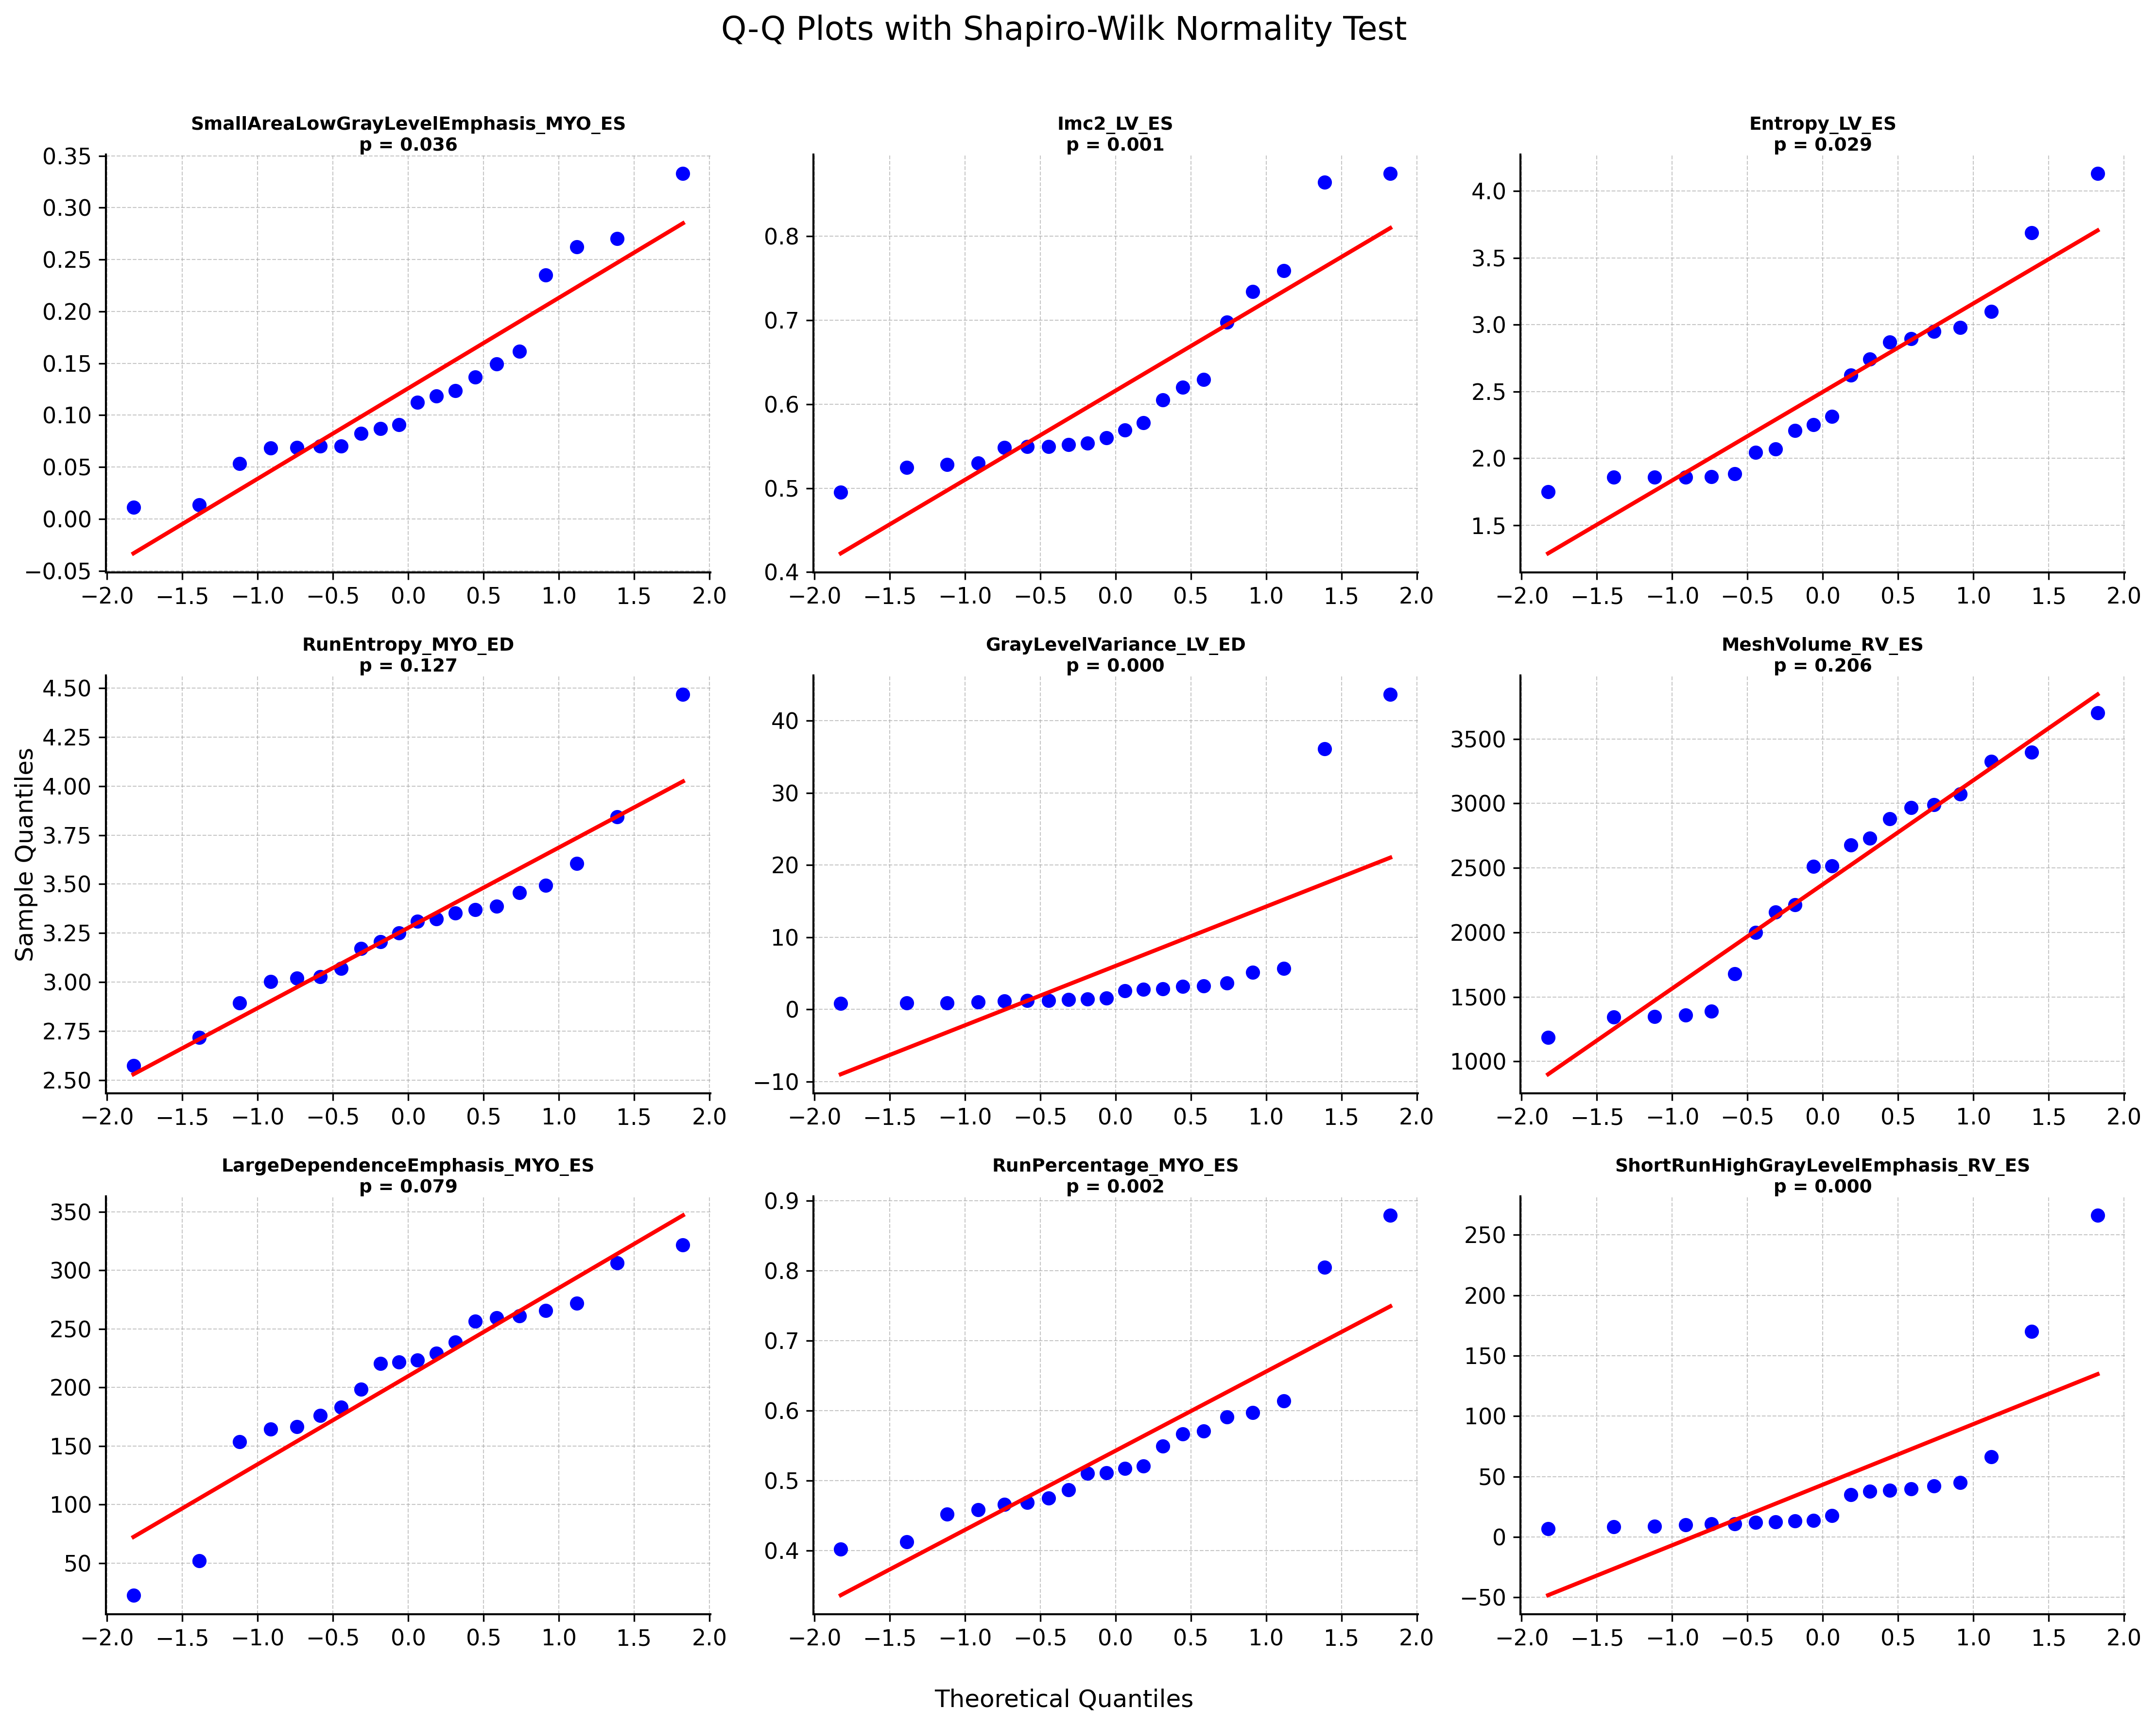
\includegraphics[width=0.85\textwidth]{../images/eda/qq.png}
	\end{center}
	\caption{Q-Q plots for randomly selected features, along with Shapiro-Wilk
		test \( p \)-values. Statistically significant is \( p < 0.05 \).}
	\label{fig:figA3}
\end{figure}

\begin{figure}
	\begin{center}
		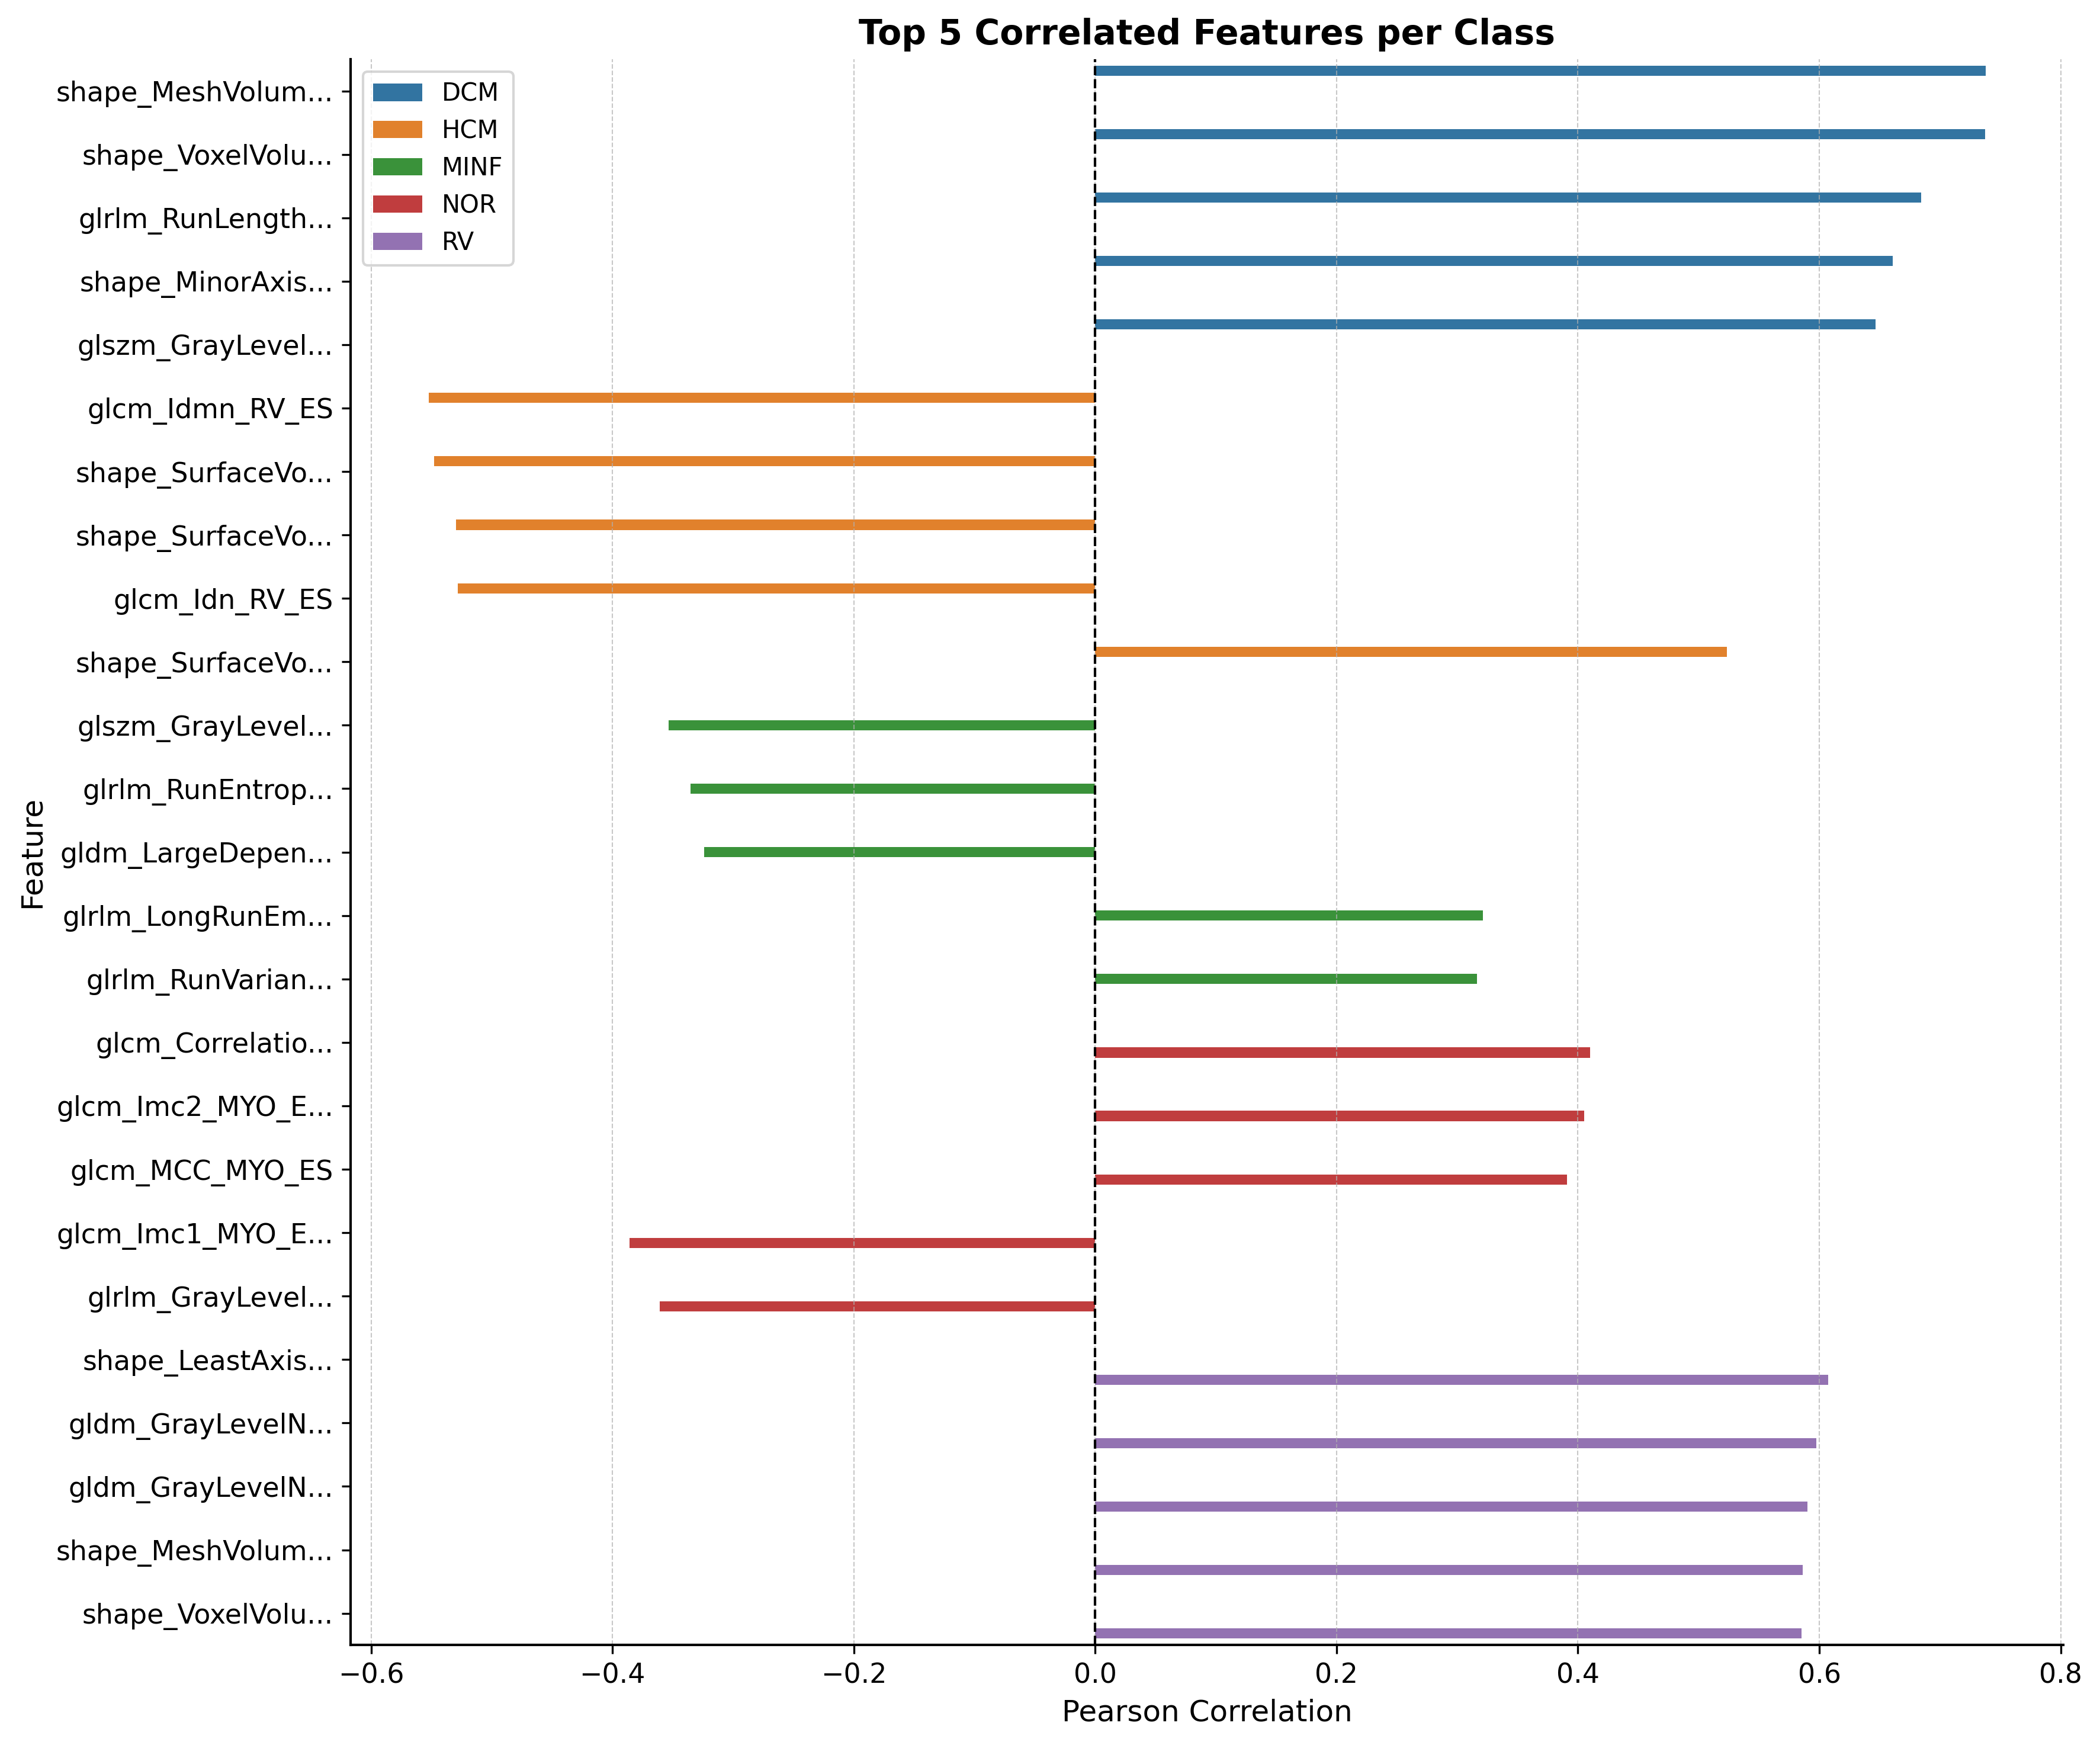
\includegraphics[width=0.82\textwidth]{../images/eda/ovr_correlation.png}
	\end{center}
	\caption{Top 5 radiomic features most correlated with each diagnostic class
		based on Pearson correlation. DCM $=$ Dilated Cardiomyopathy, HCM $=$
		Hypertrophic Cardiomyopathy, MINF $=$ Myocardial Infarction, NOR $=$ Normal, RV
		$=$ Right Ventricular abnormality.}
	\label{fig:figA4}
\end{figure}

\begin{figure}
	\begin{center}
		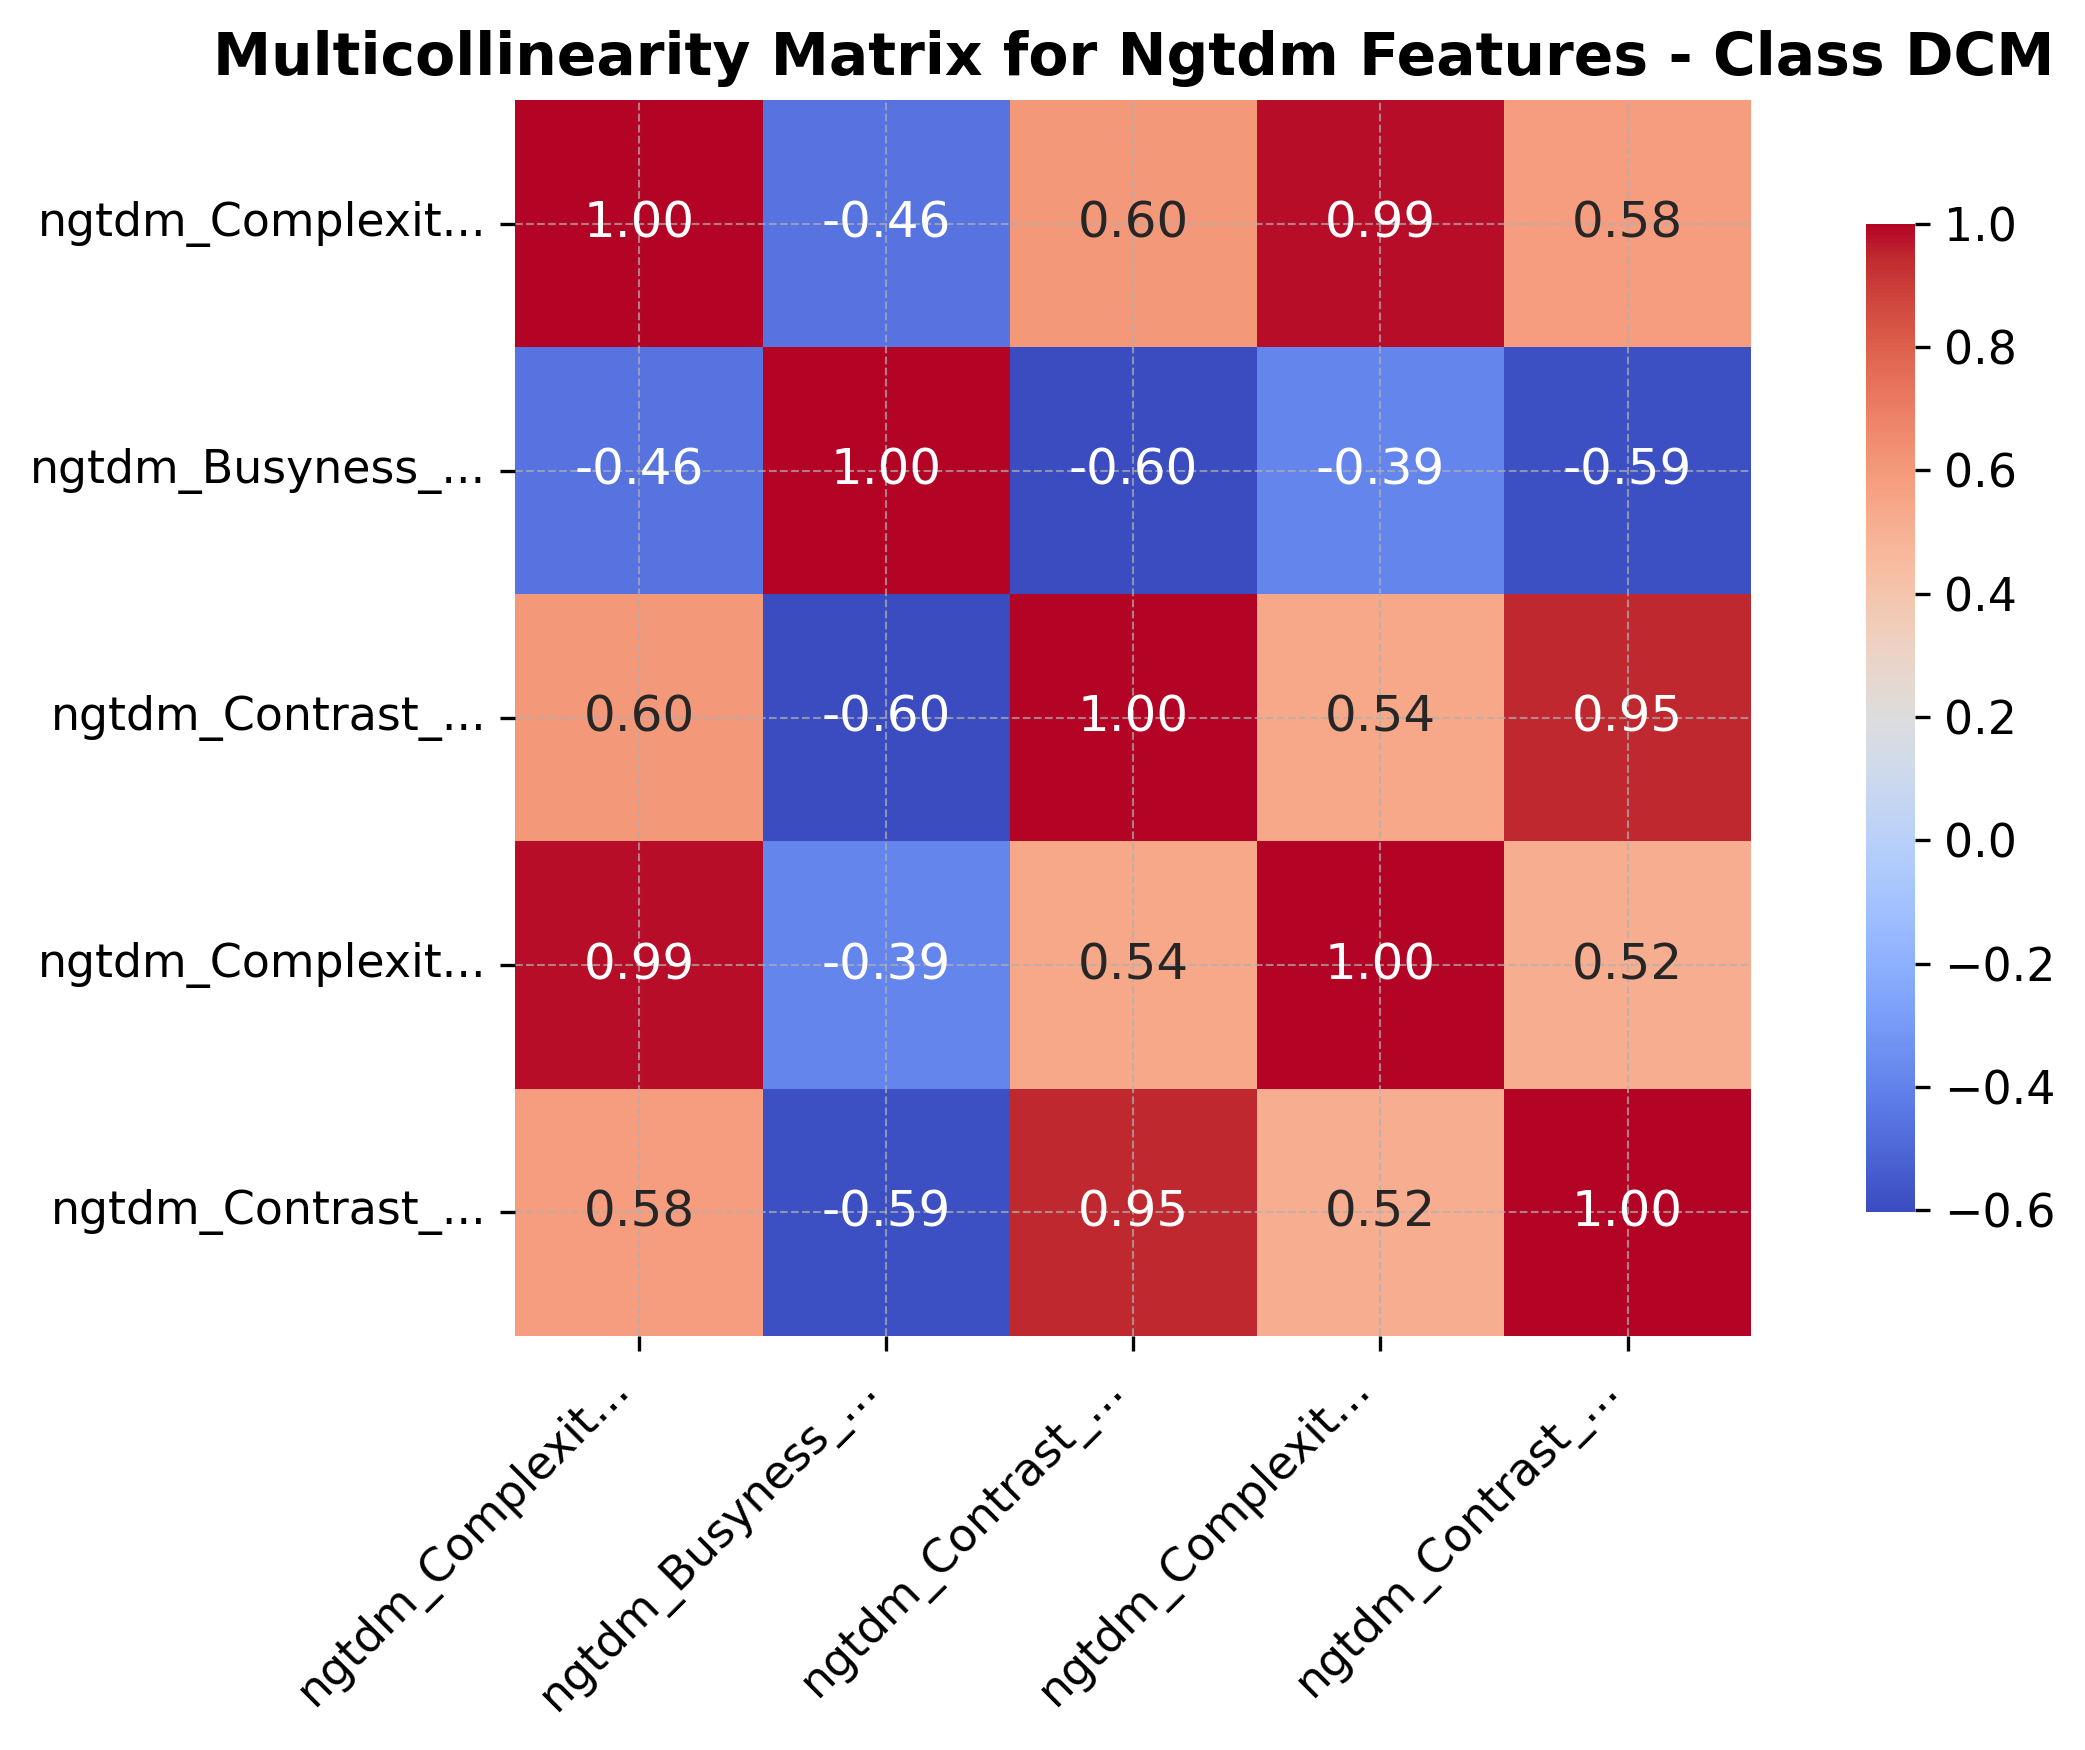
\includegraphics[width=0.85\textwidth]{../images/eda/multicollinearity.png}
	\end{center}
	\caption{Multicollinearity matrix for five randomly selected Ngtdm features
		in the Dilated Cardiomyopathy (DCM) class.}
	\label{fig:figA5}
\end{figure}

\begin{figure}
	\begin{center}
		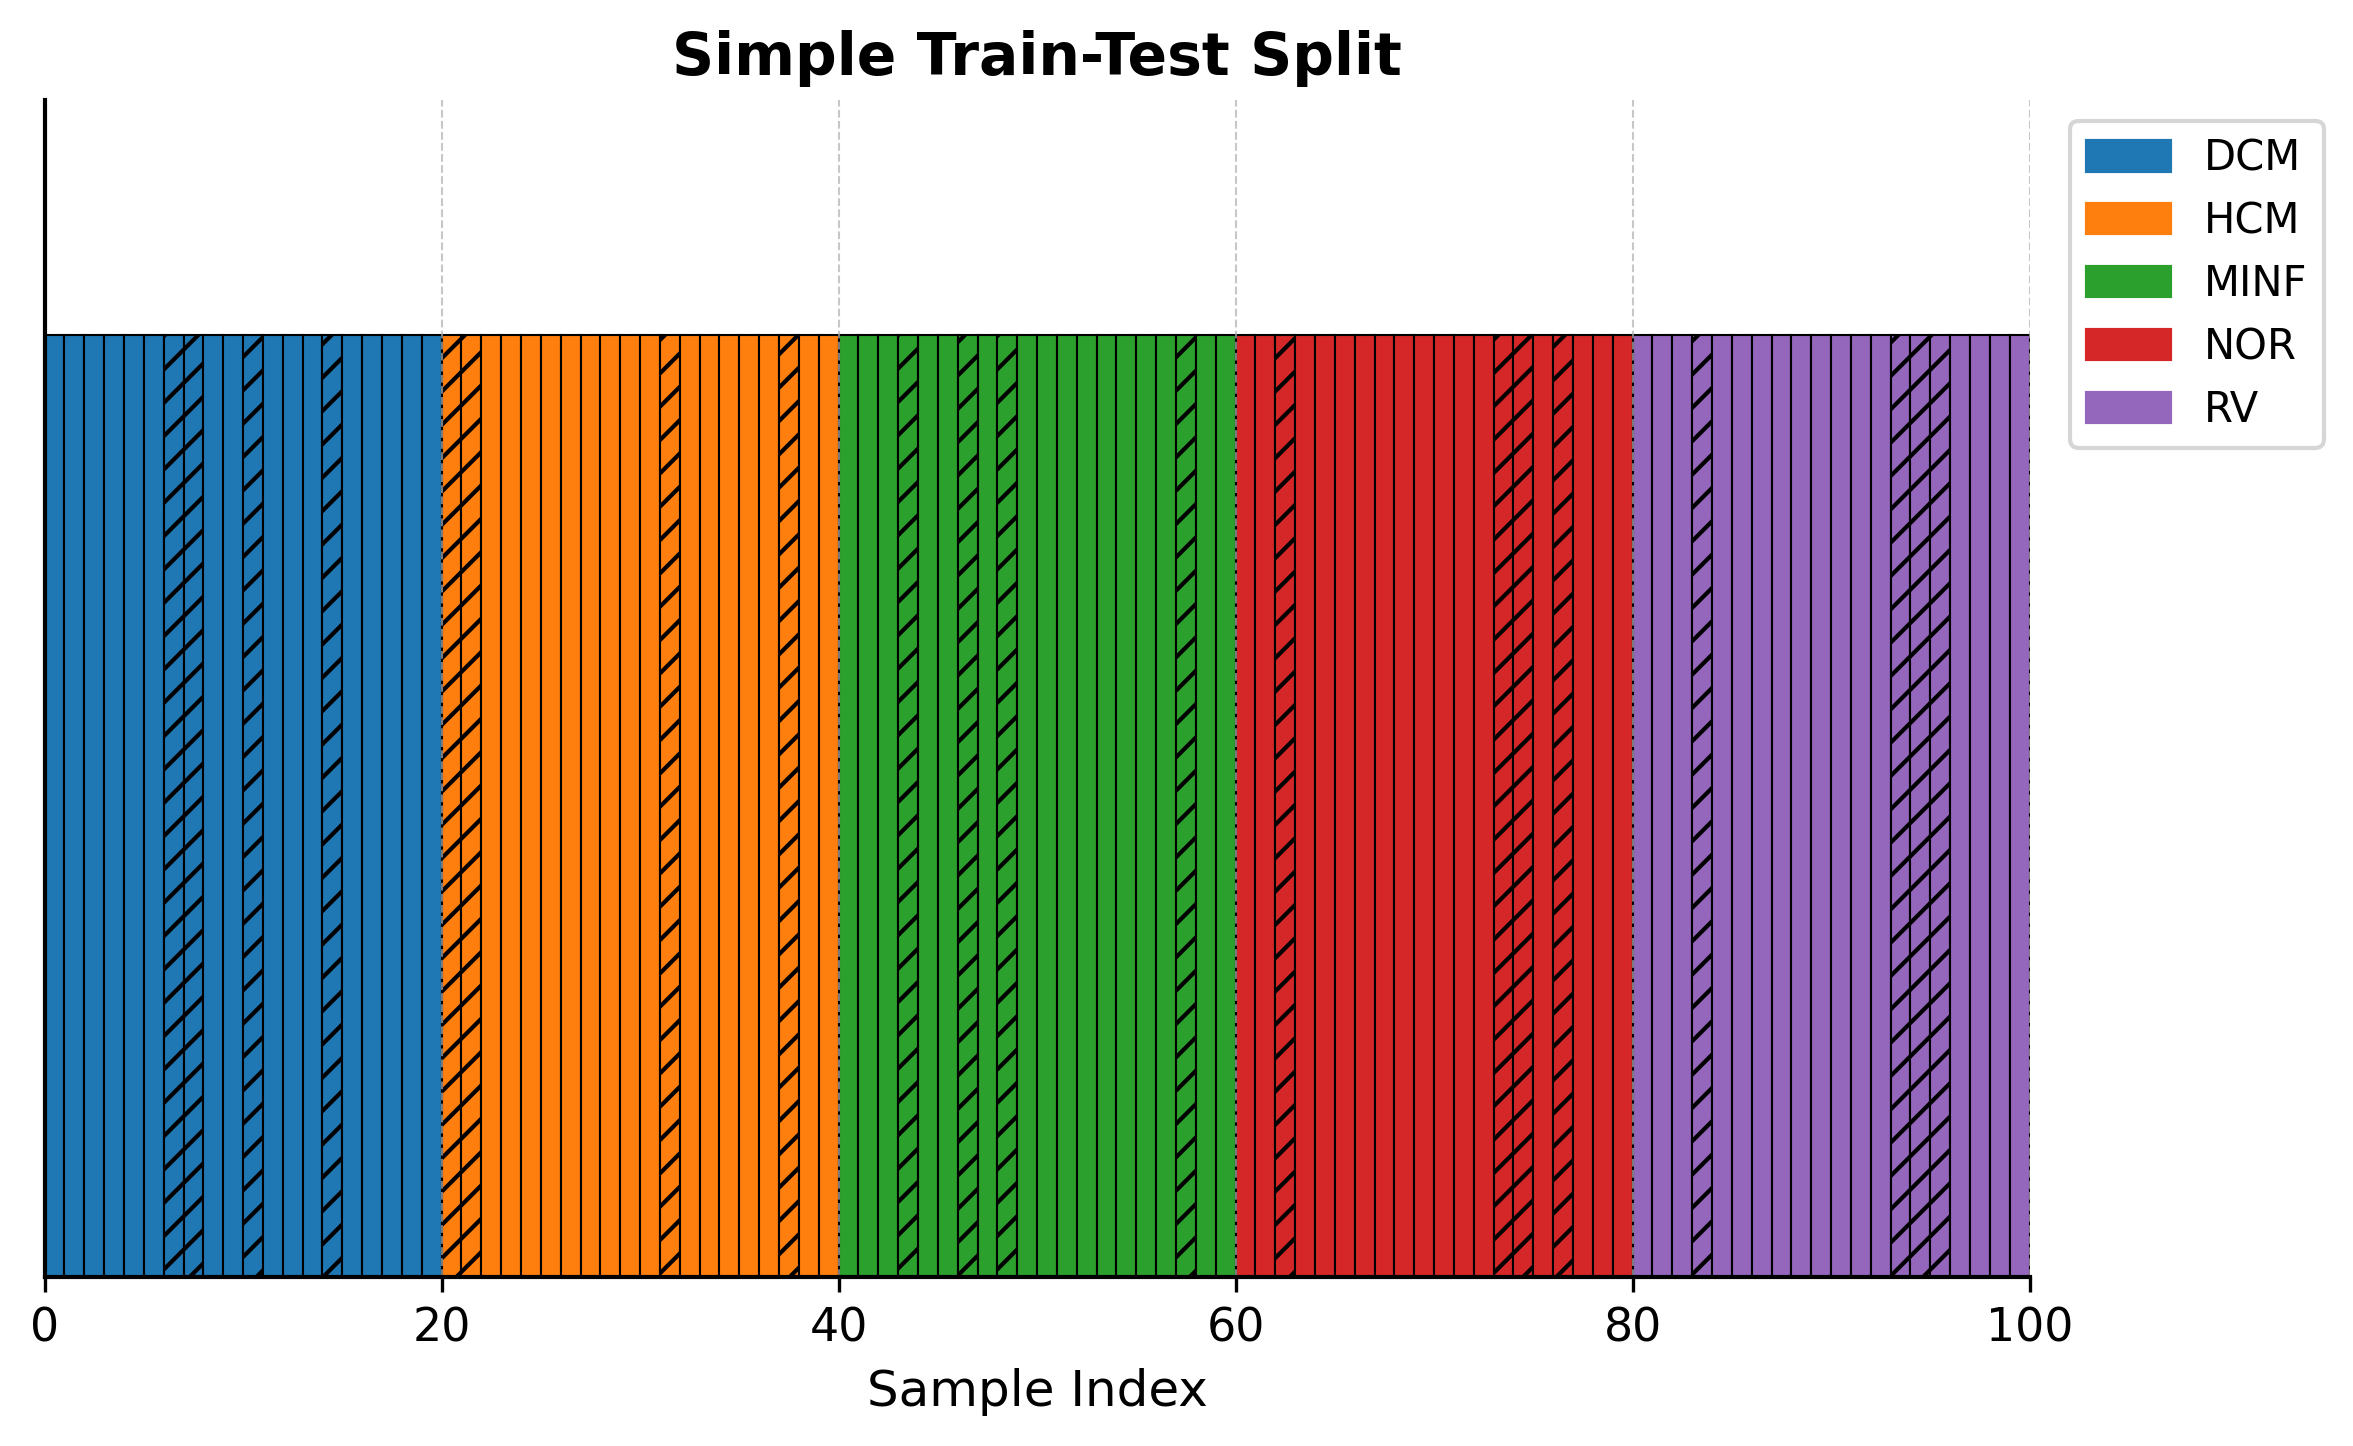
\includegraphics[width=0.99\textwidth]{../images/splits/simple.png}
	\end{center}
	\caption{Visualization of the Simple Split strategy. Each color represents a
		different class, and hatched bars indicate validation samples. DCM $=$
		Dilated Cardiomyopathy, HCM $=$ Hypertrophic Cardiomyopathy, MINF $=$
		Myocardial Infarction, NOR $=$ Normal, RV $=$ Right Ventricular abnormality.}
	\label{fig:figA6}
\end{figure}

\begin{figure}
	\begin{center}
		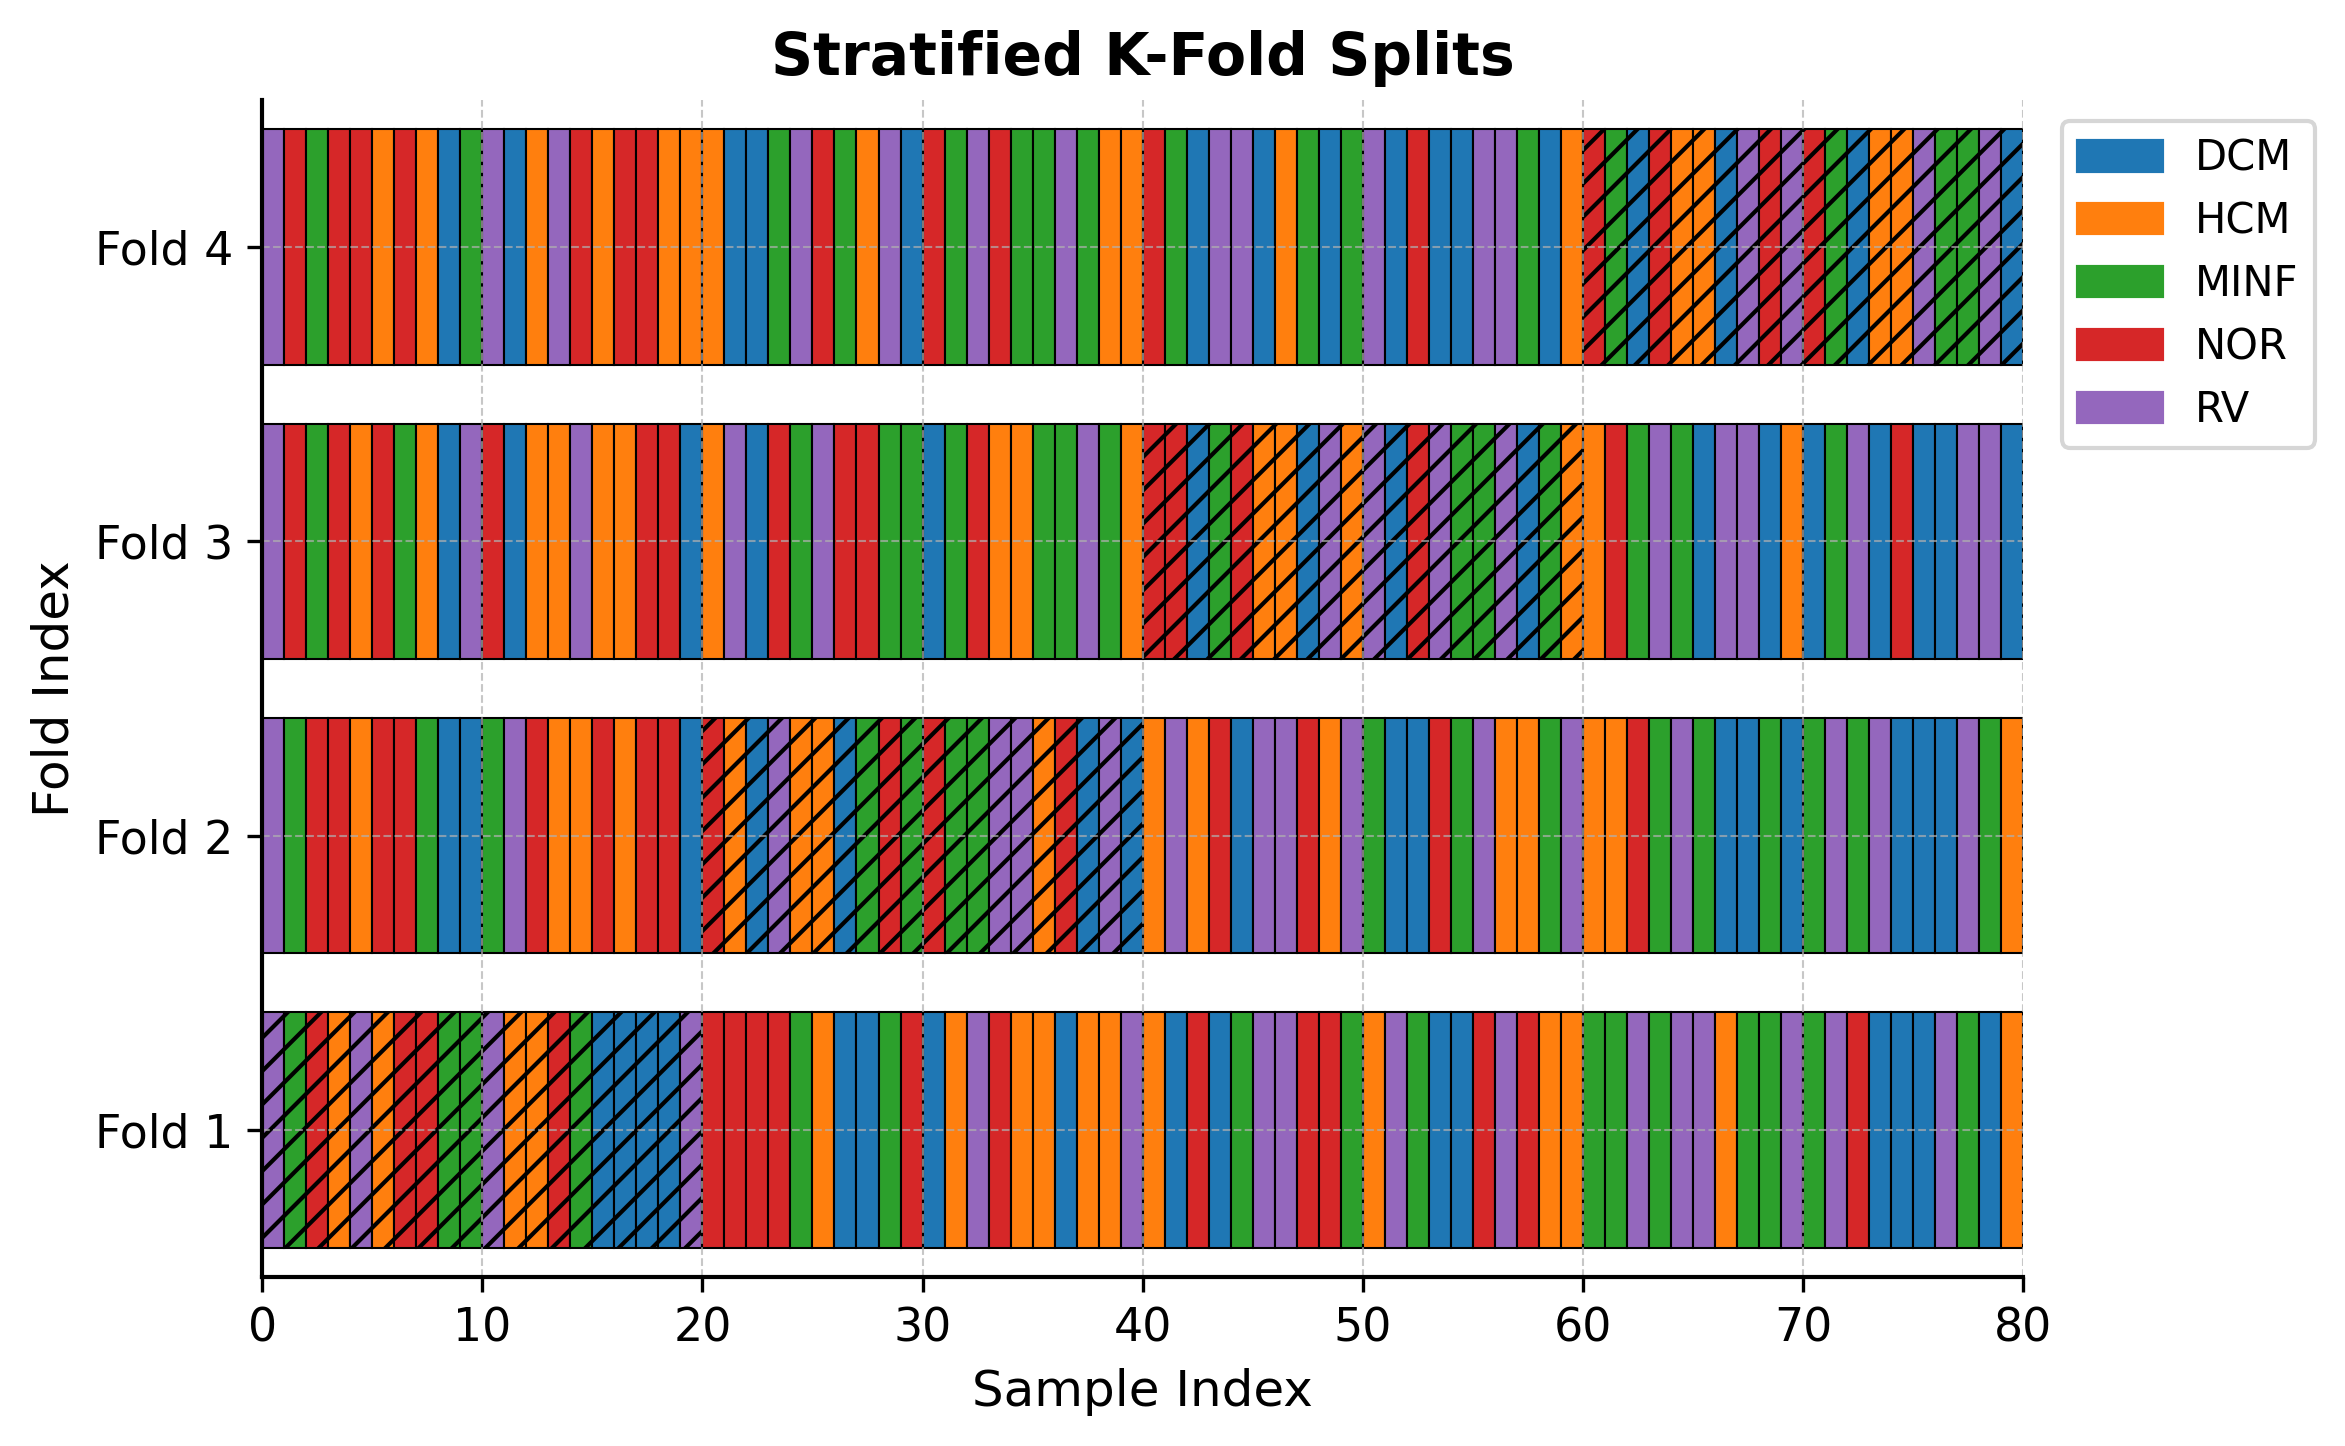
\includegraphics[width=0.99\textwidth]{../images/splits/kfold.png}
	\end{center}
	\caption{Visualization of the Stratified K-Fold cross-validation splits. Each
		color represents a different class, and hatched bars indicate validation
		samples. DCM $=$ Dilated Cardiomyopathy, HCM $=$ Hypertrophic
		Cardiomyopathy, MINF $=$ Myocardial Infarction, NOR $=$ Normal, RV $=$
		Right Ventricular abnormality.}
	\label{fig:figA7}
\end{figure}

\begin{figure}
	\begin{center}
		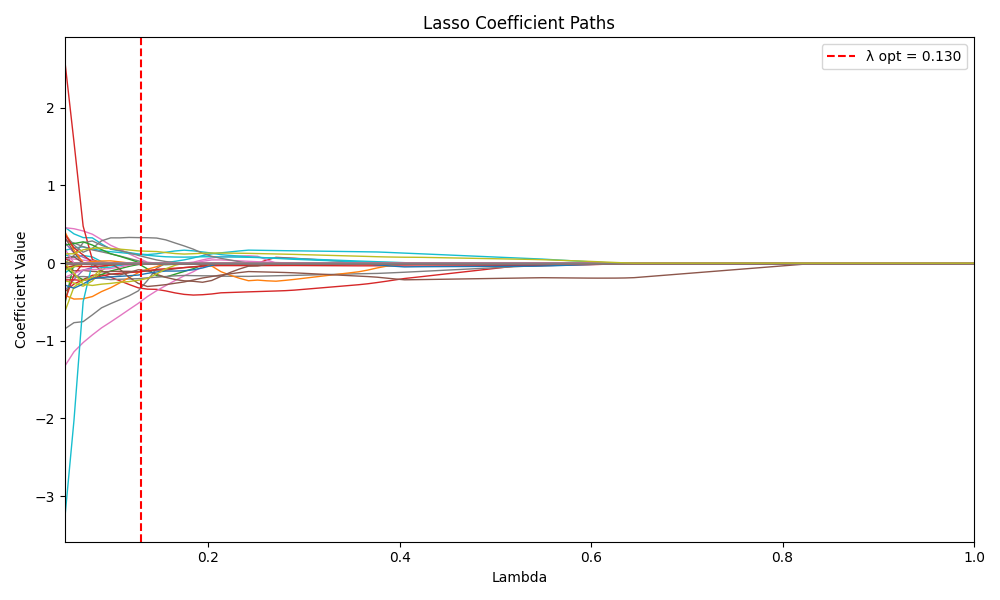
\includegraphics[width=0.99\textwidth]{../images/lasso/coeff_vs_lambda.png}
	\end{center}
	\caption{LASSO coefficient paths across varying \(\lambda\) values. The red
		dashed line indicates the selected optimal \(\lambda_{\text{opt}}\)
		minimizing validation error.}
	\label{fig:figA8}
\end{figure}

\begin{figure}
	\begin{center}
		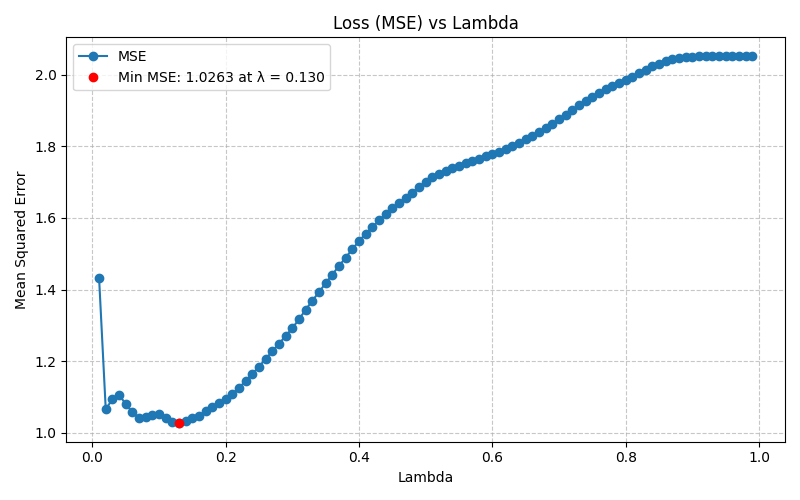
\includegraphics[width=0.99\textwidth]{../images/lasso/mse_vs_lambda.png}
	\end{center}
	\caption{Mean Squared Error (MSE) as a function of \(\lambda\). The minimum
		MSE is marked at the optimal regularization parameter
		\(\lambda_{\text{opt}}\).}
	\label{fig:figA9}
\end{figure}

\begin{figure}
	\begin{center}
		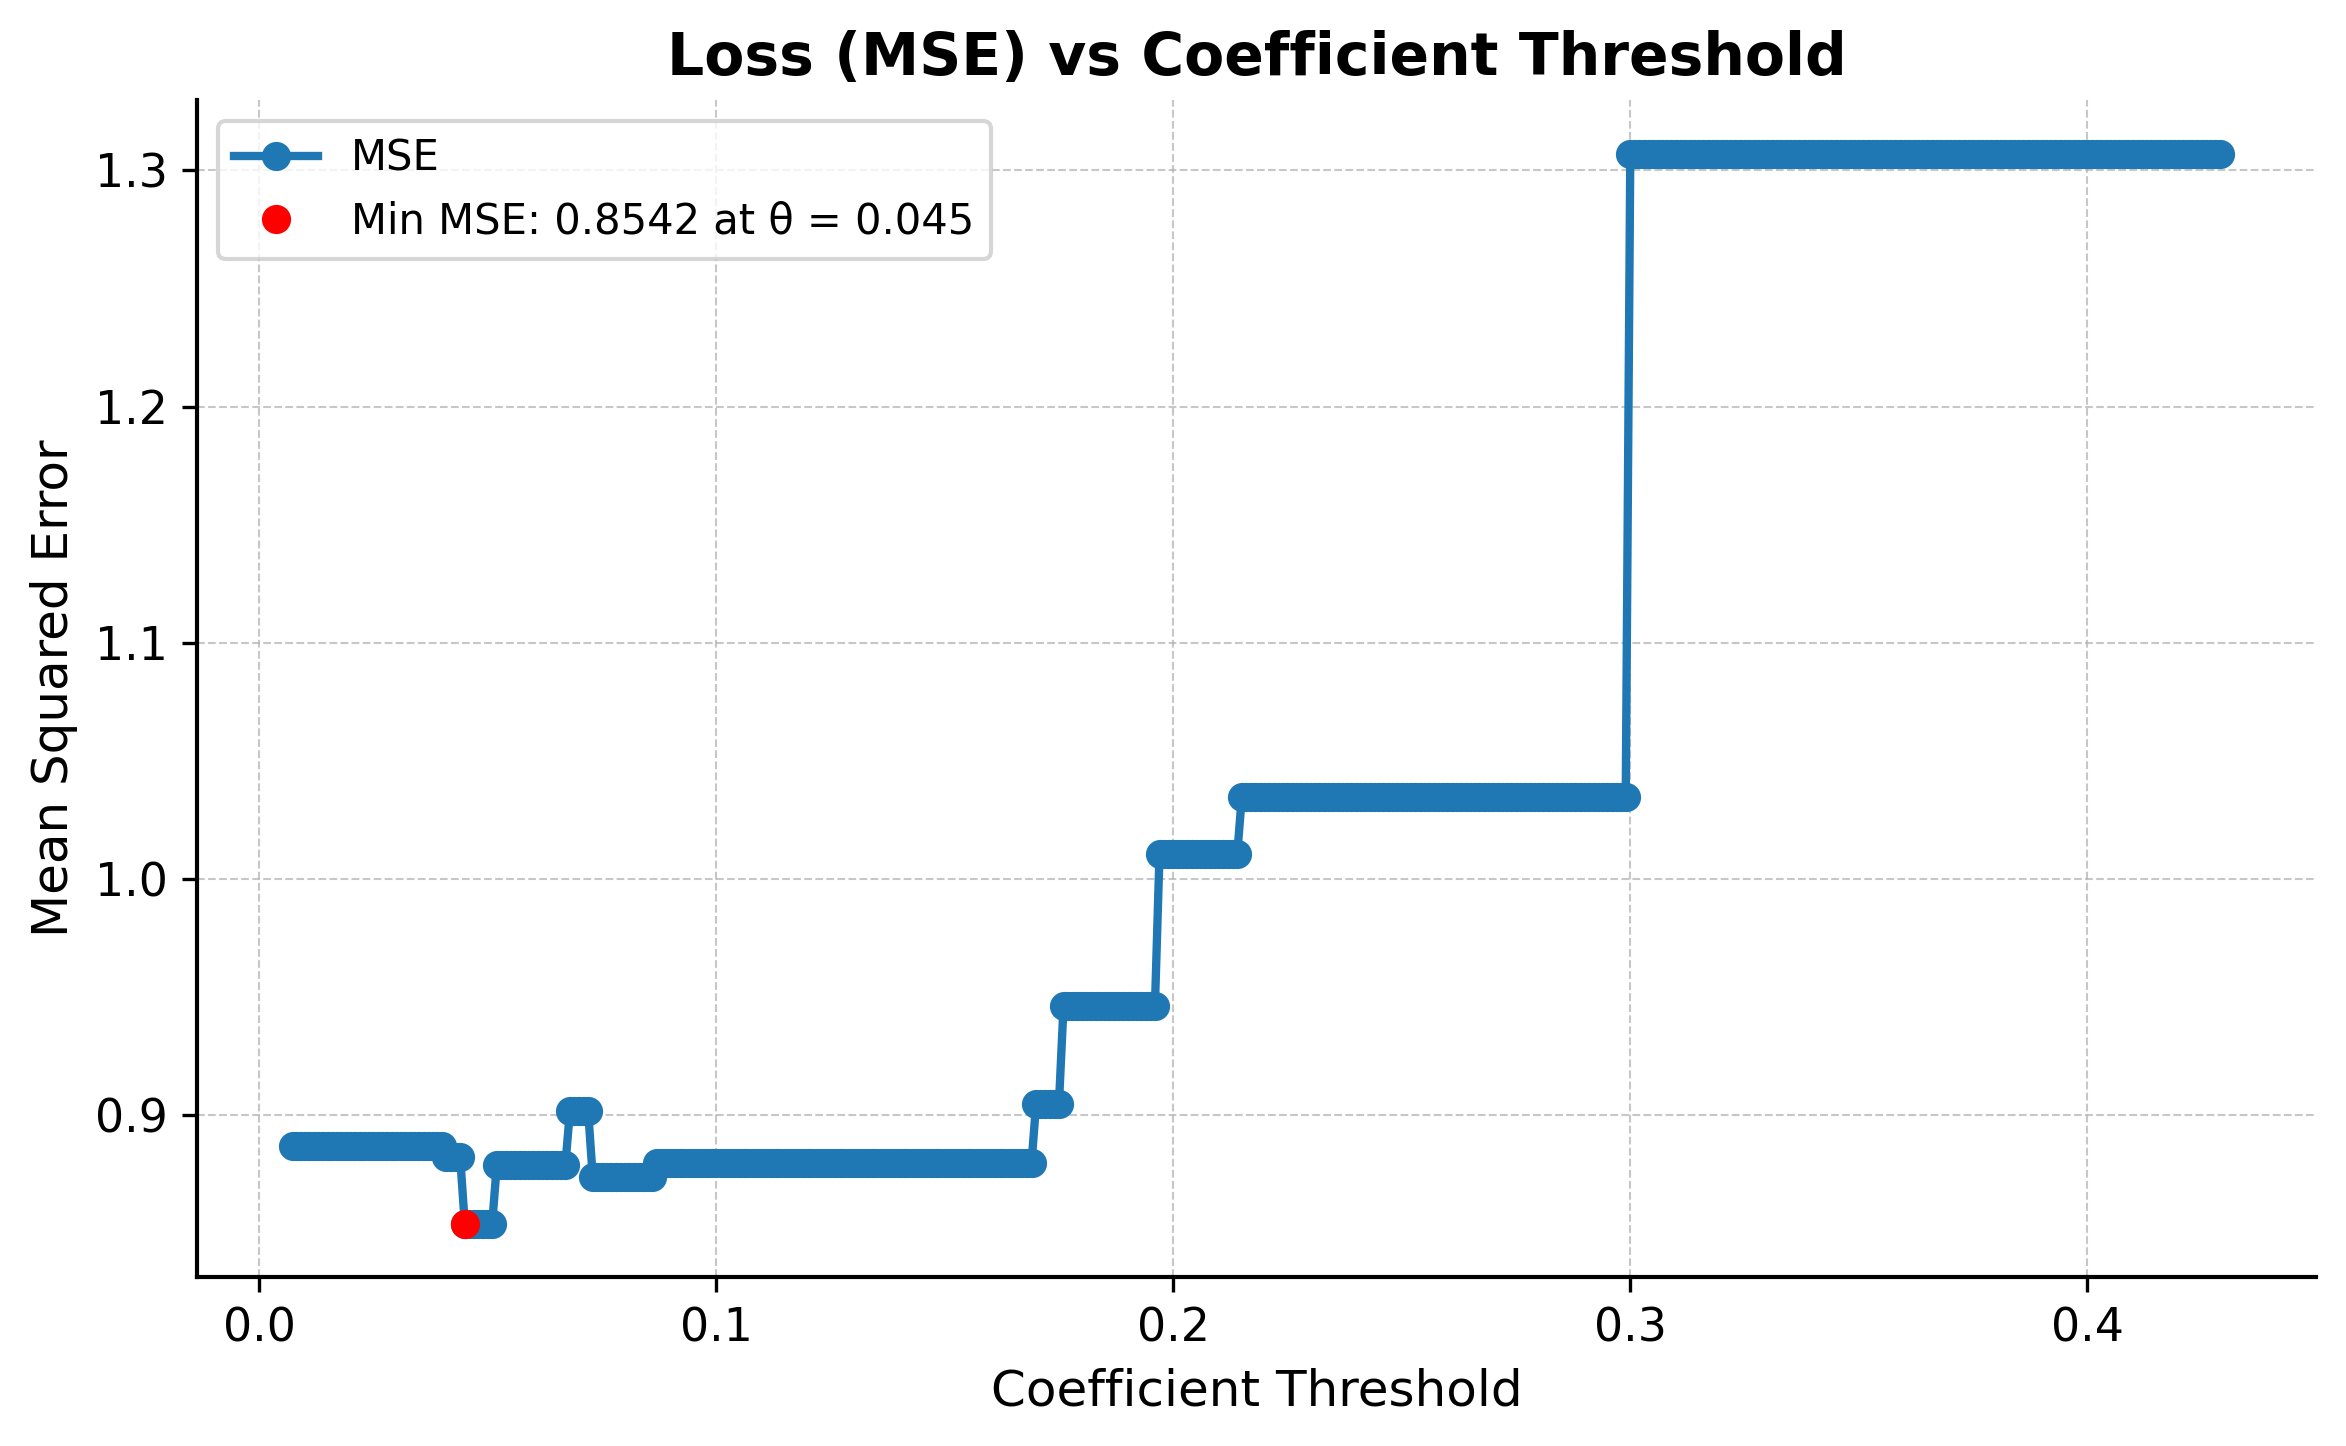
\includegraphics[width=0.99\textwidth]{../images/lasso/mse_vs_threshold.png}
	\end{center}
	\caption{Mean Squared Error (MSE) as a function of the coefficient threshold
	\(\text{coe\_thr}\) after LASSO fitting. The optimal threshold
	\(\text{coe\_thr}_{\text{opt}}\) corresponds to the minimum MSE.}
	\label{fig:figA10}
\end{figure}

\begin{figure}
	\begin{center}
		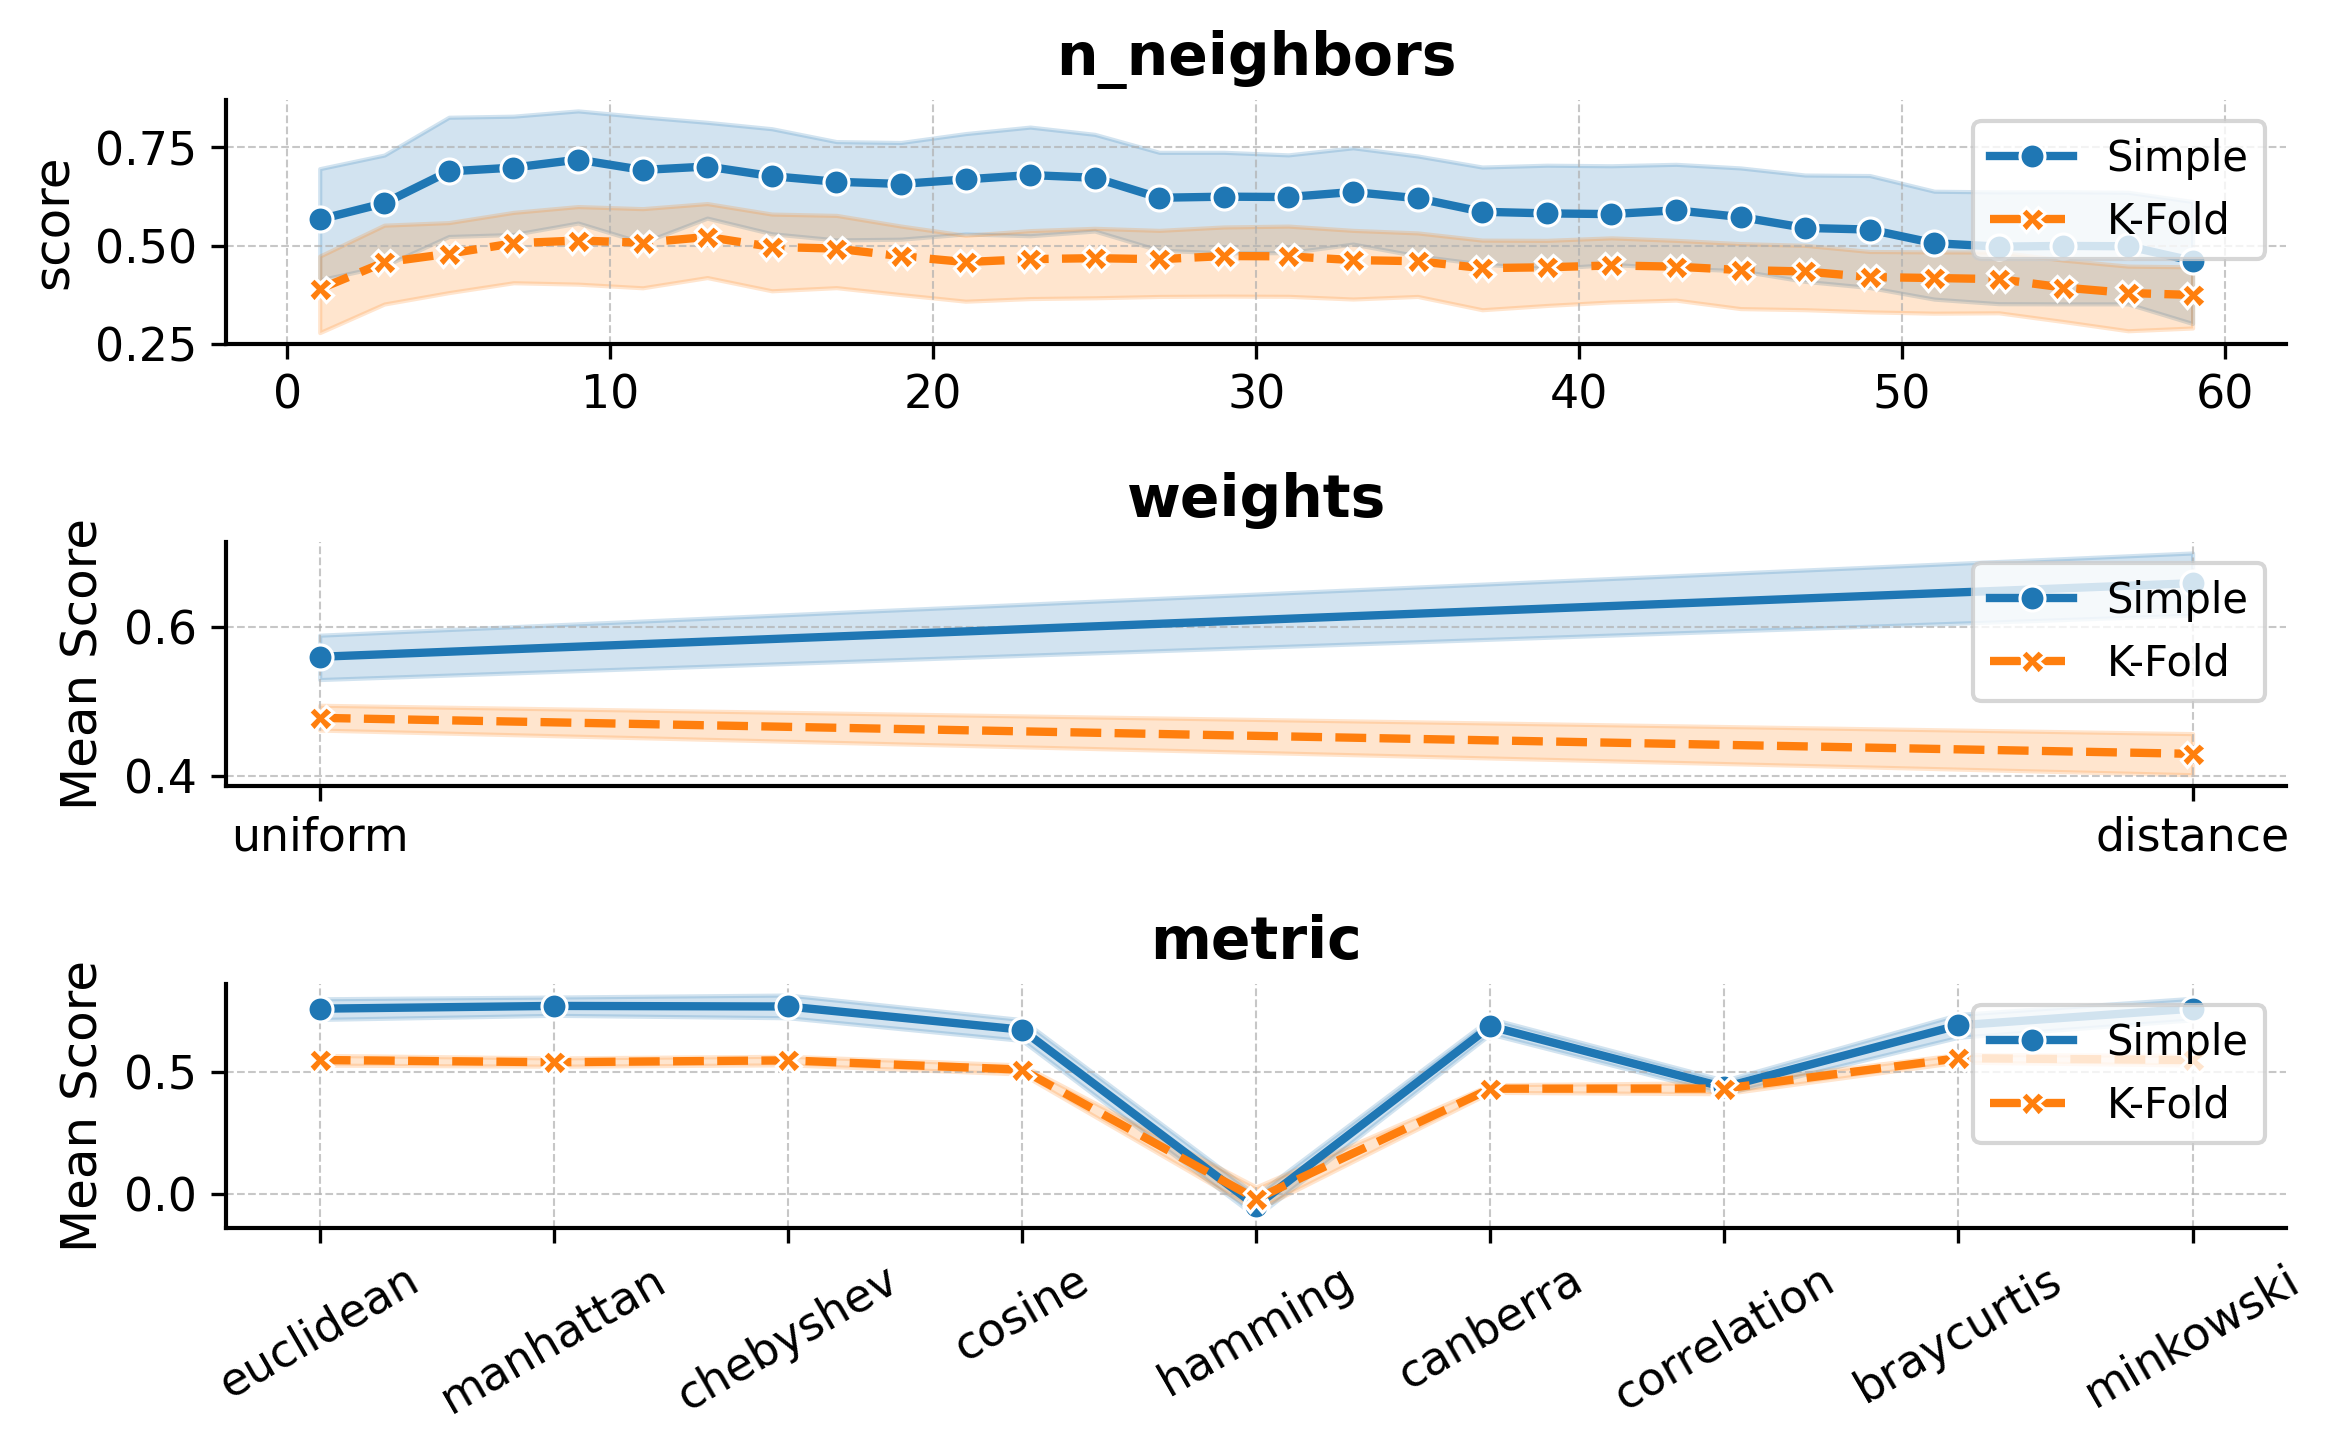
\includegraphics[width=0.99\textwidth]{../images/models/knn_hyperparameters_evolution.png}
	\end{center}
	\caption{Hyperparameter evolution for the k-Nearest Neighbors (KNN) model
		across different values.}
	\label{fig:figA11}
\end{figure}

\begin{figure}
	\begin{center}
		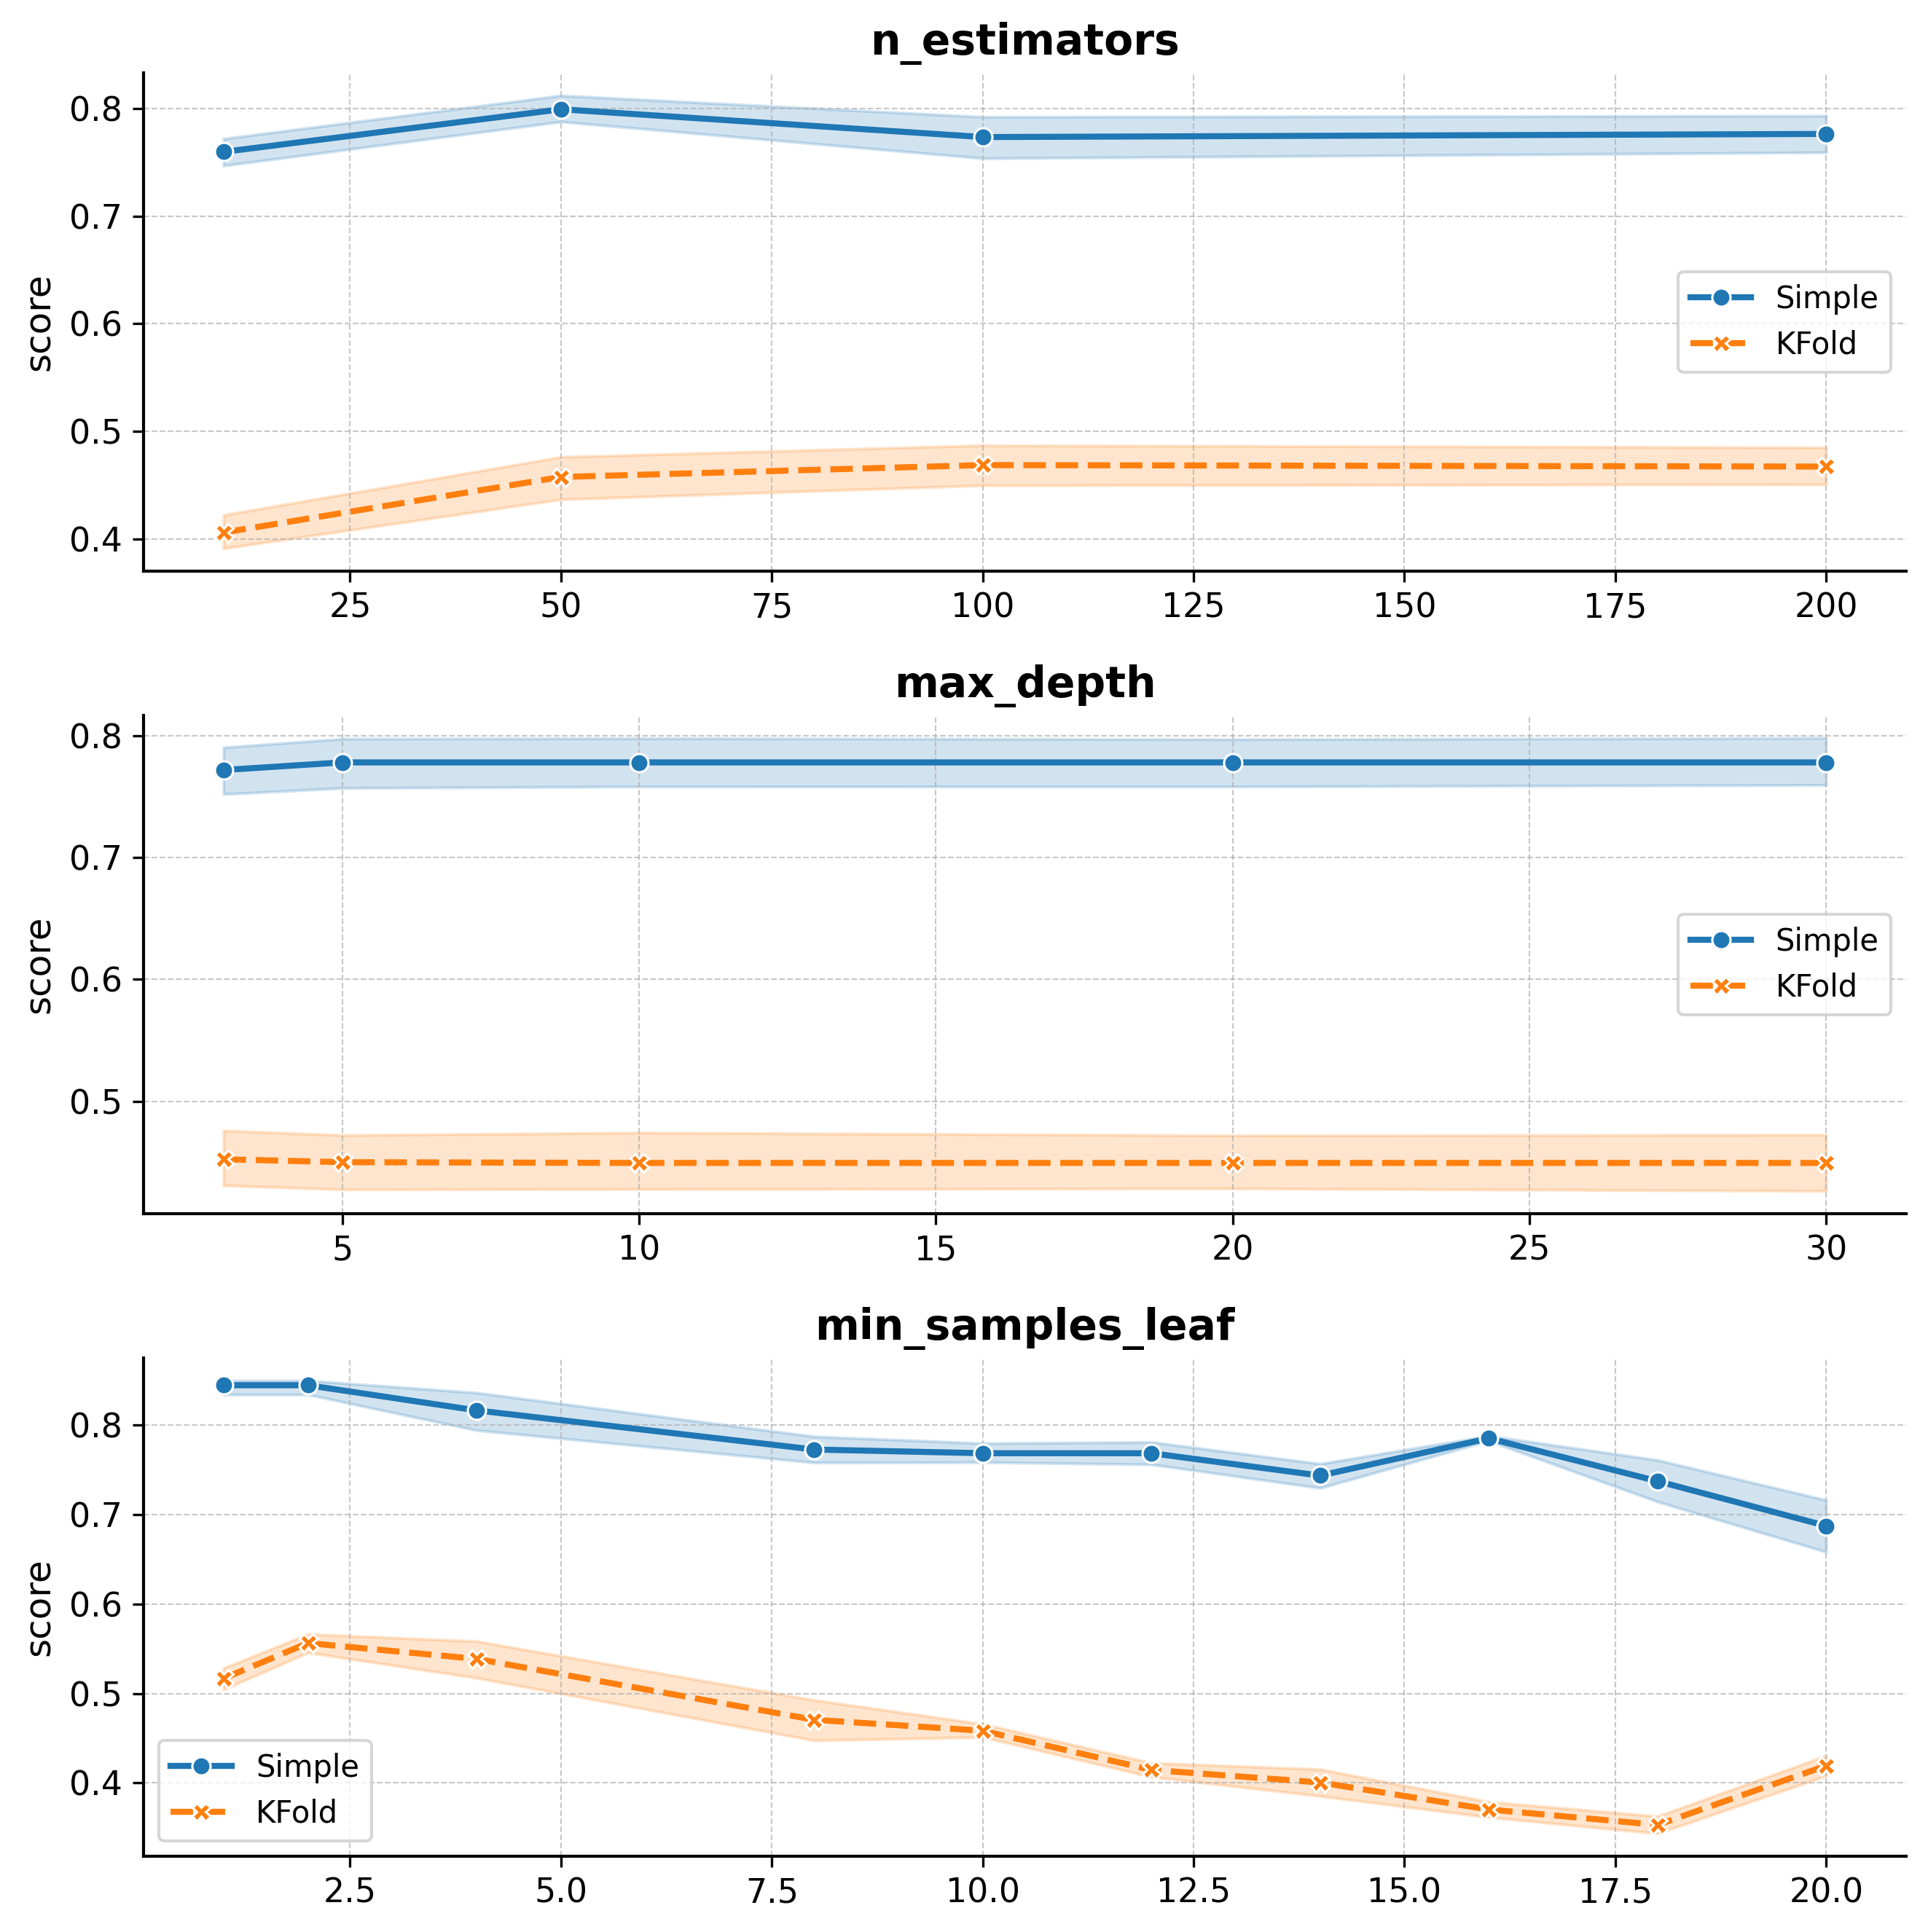
\includegraphics[width=0.99\textwidth]{../images/models/rf_hyperparameters_evolution.png}
	\end{center}
	\caption{Hyperparameter evolution for the Random Forest (RF) model across
		different values.}
\end{figure}

\begin{figure}
	\begin{center}
		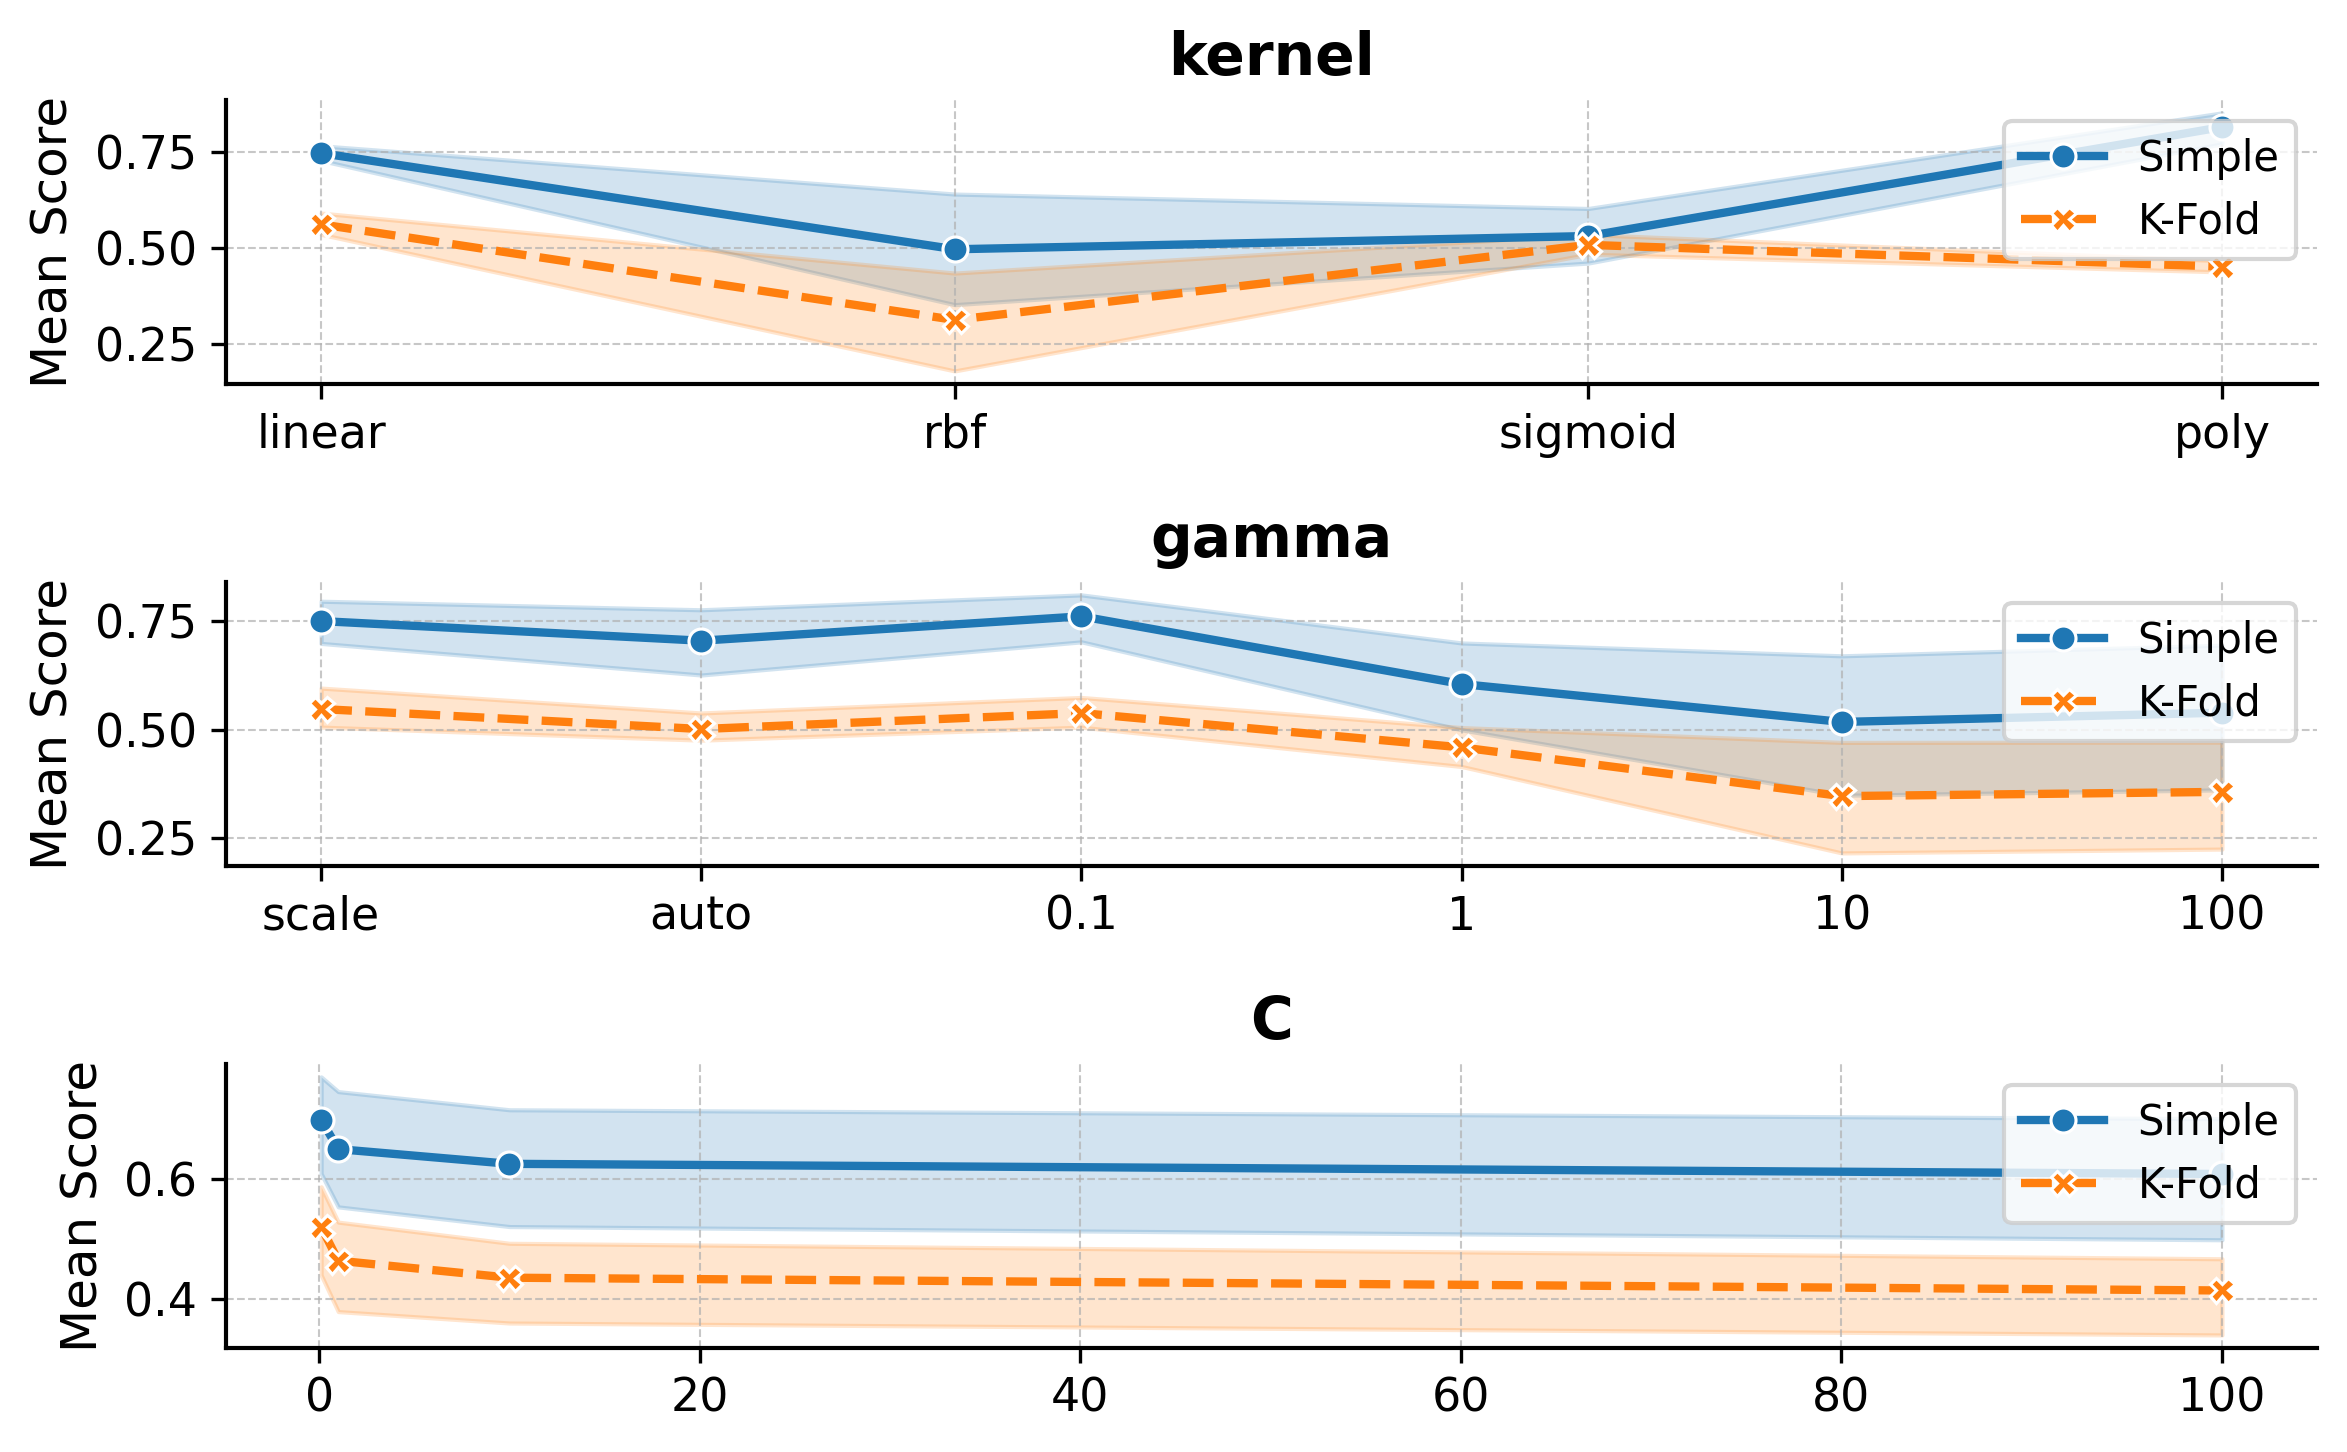
\includegraphics[width=0.99\textwidth]{../images/models/svm_hyperparameters_evolution.png}
	\end{center}
	\caption{Hyperparameter evolution for the Support Vector Machine (SVM) model
		across different values.}
\end{figure}

\begin{figure}
	\begin{center}
		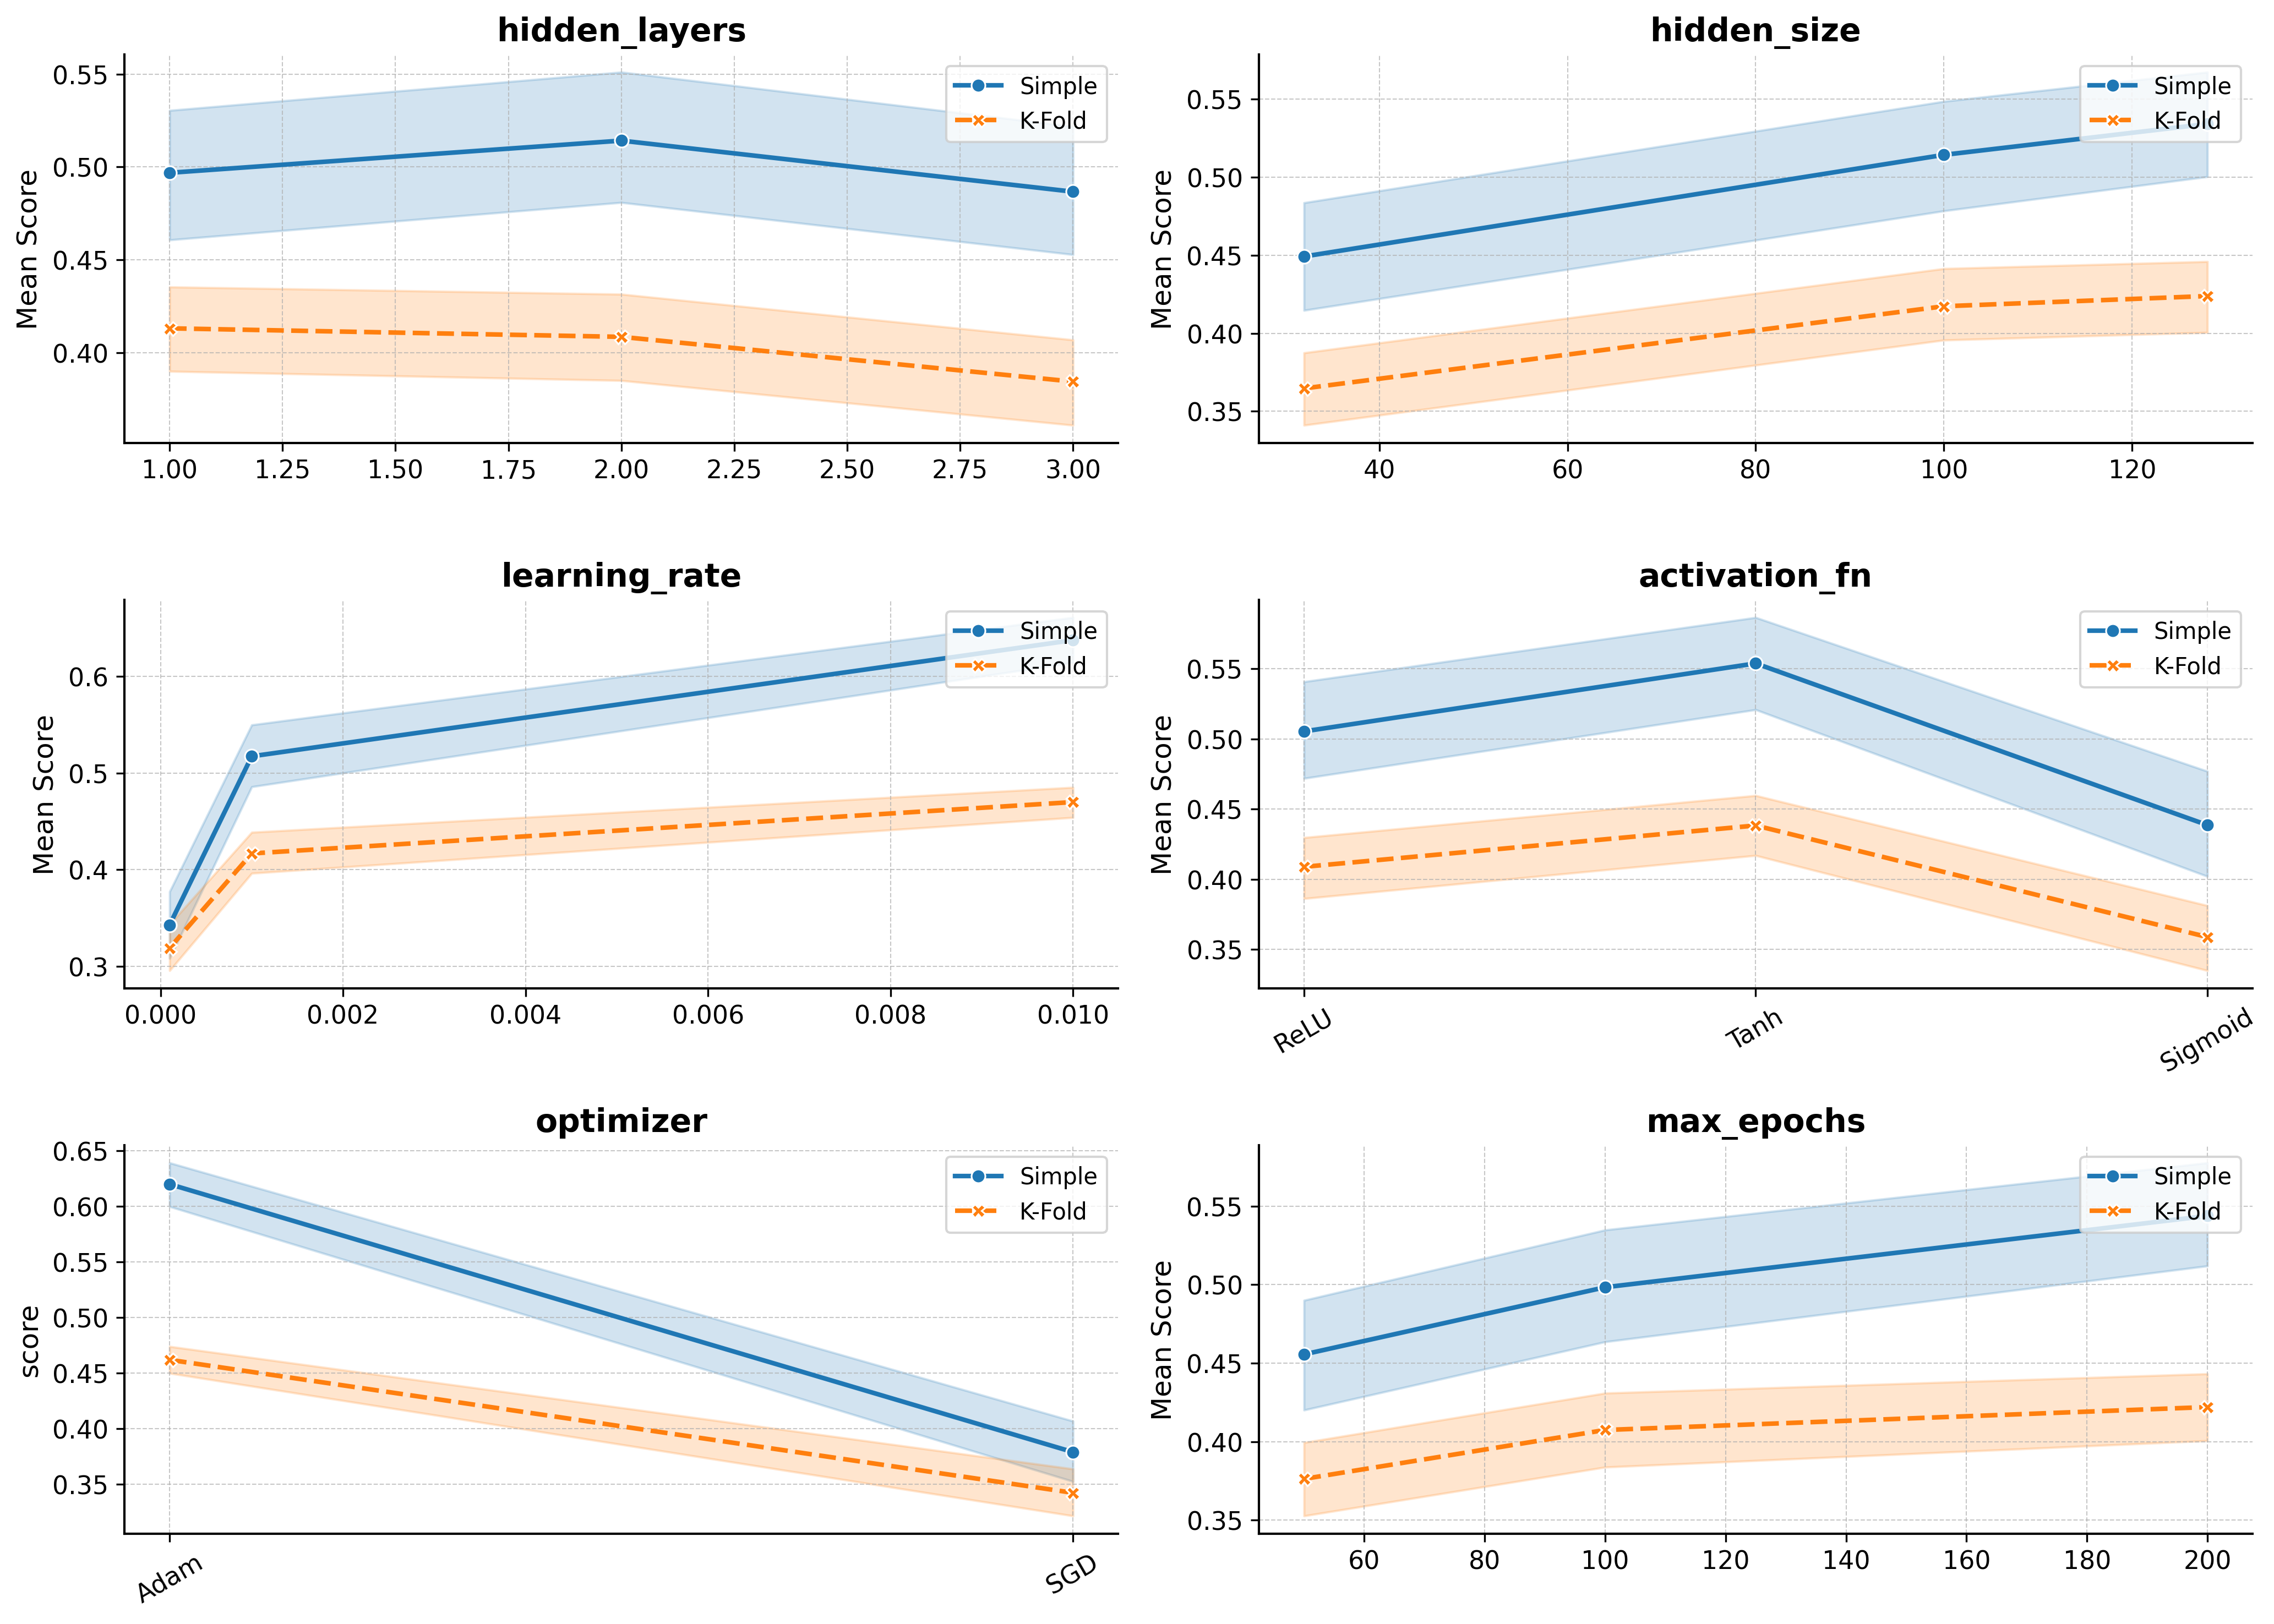
\includegraphics[width=0.99\textwidth]{../images/models/ann_hyperparameters_evolution.png}
	\end{center}
	\caption{Hyperparameter evolution for the Artificial Neural Network (ANN)
		model across different values.}
	\label{fig:figA14}
\end{figure}

\begin{figure}
	\begin{center}
		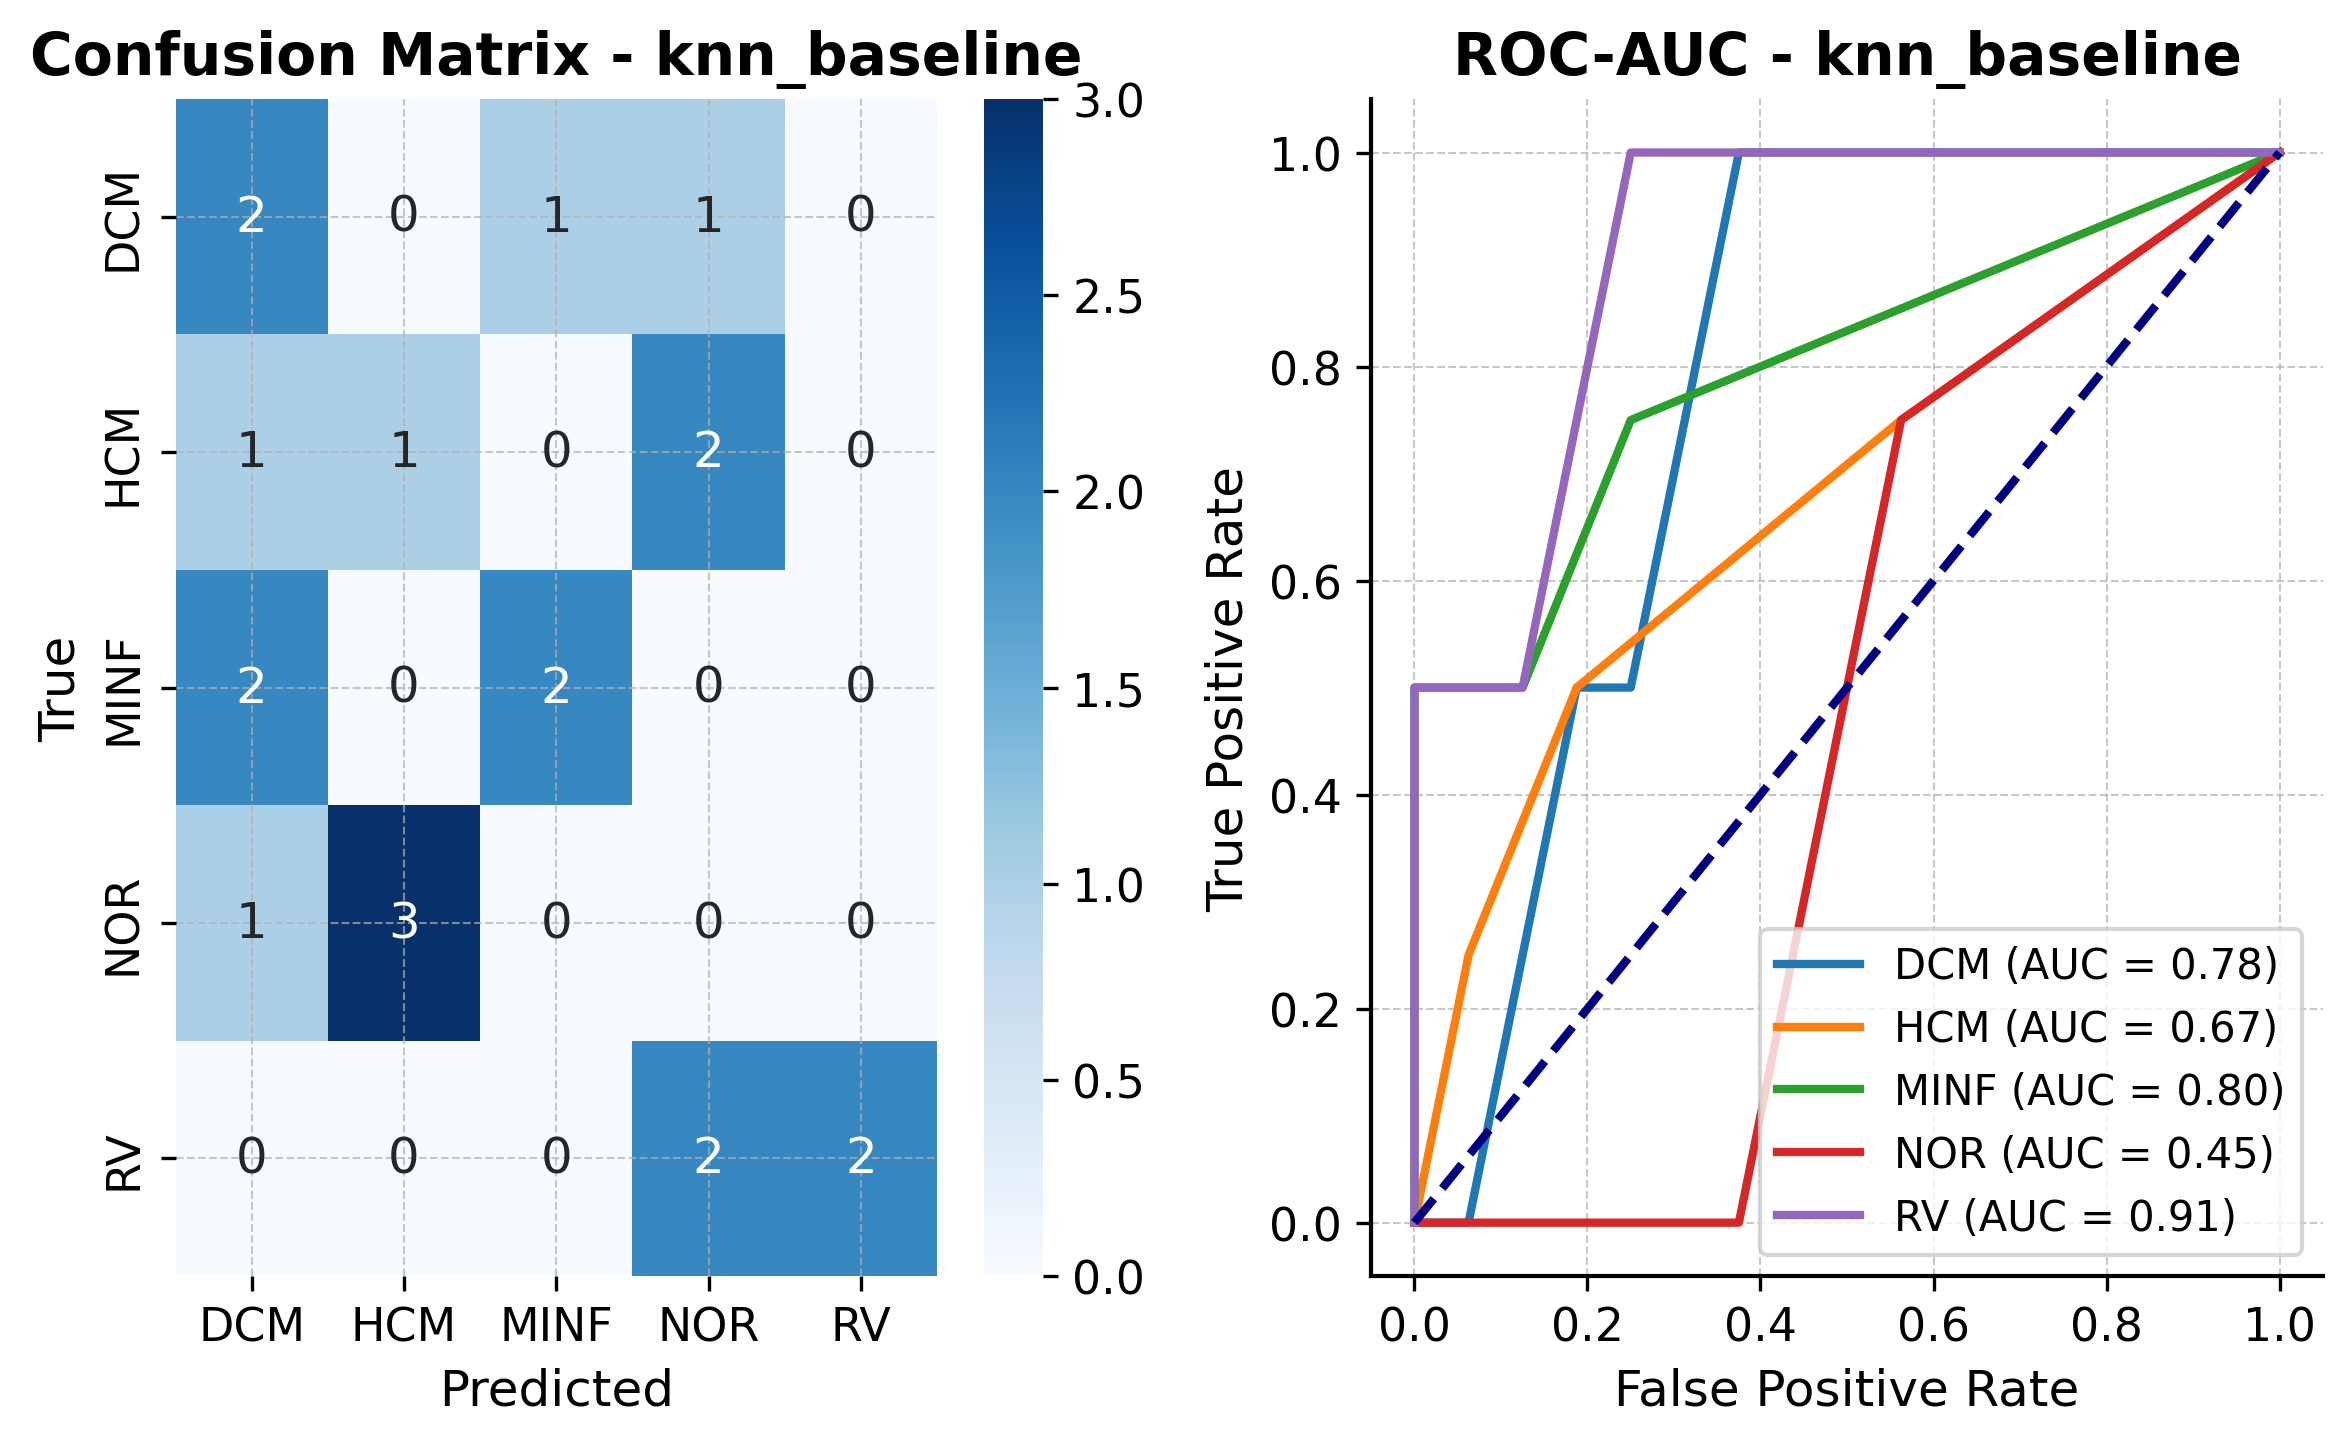
\includegraphics[width=0.99\textwidth]{../images/metrics/knn/knn_baseline_metrics.png}
	\end{center}
	\caption{Confusion matrix and ROC curves for the k-Nearest Neighbors (KNN)
		model trained using no strategy. DCM $=$ Dilated Cardiomyopathy, HCM $=$
		Hypertrophic Cardiomyopathy, MINF $=$ Myocardial Infarction, NOR $=$ Normal, RV
		$=$ Right Ventricular abnormality.}
\end{figure}

\begin{figure}
	\begin{center}
		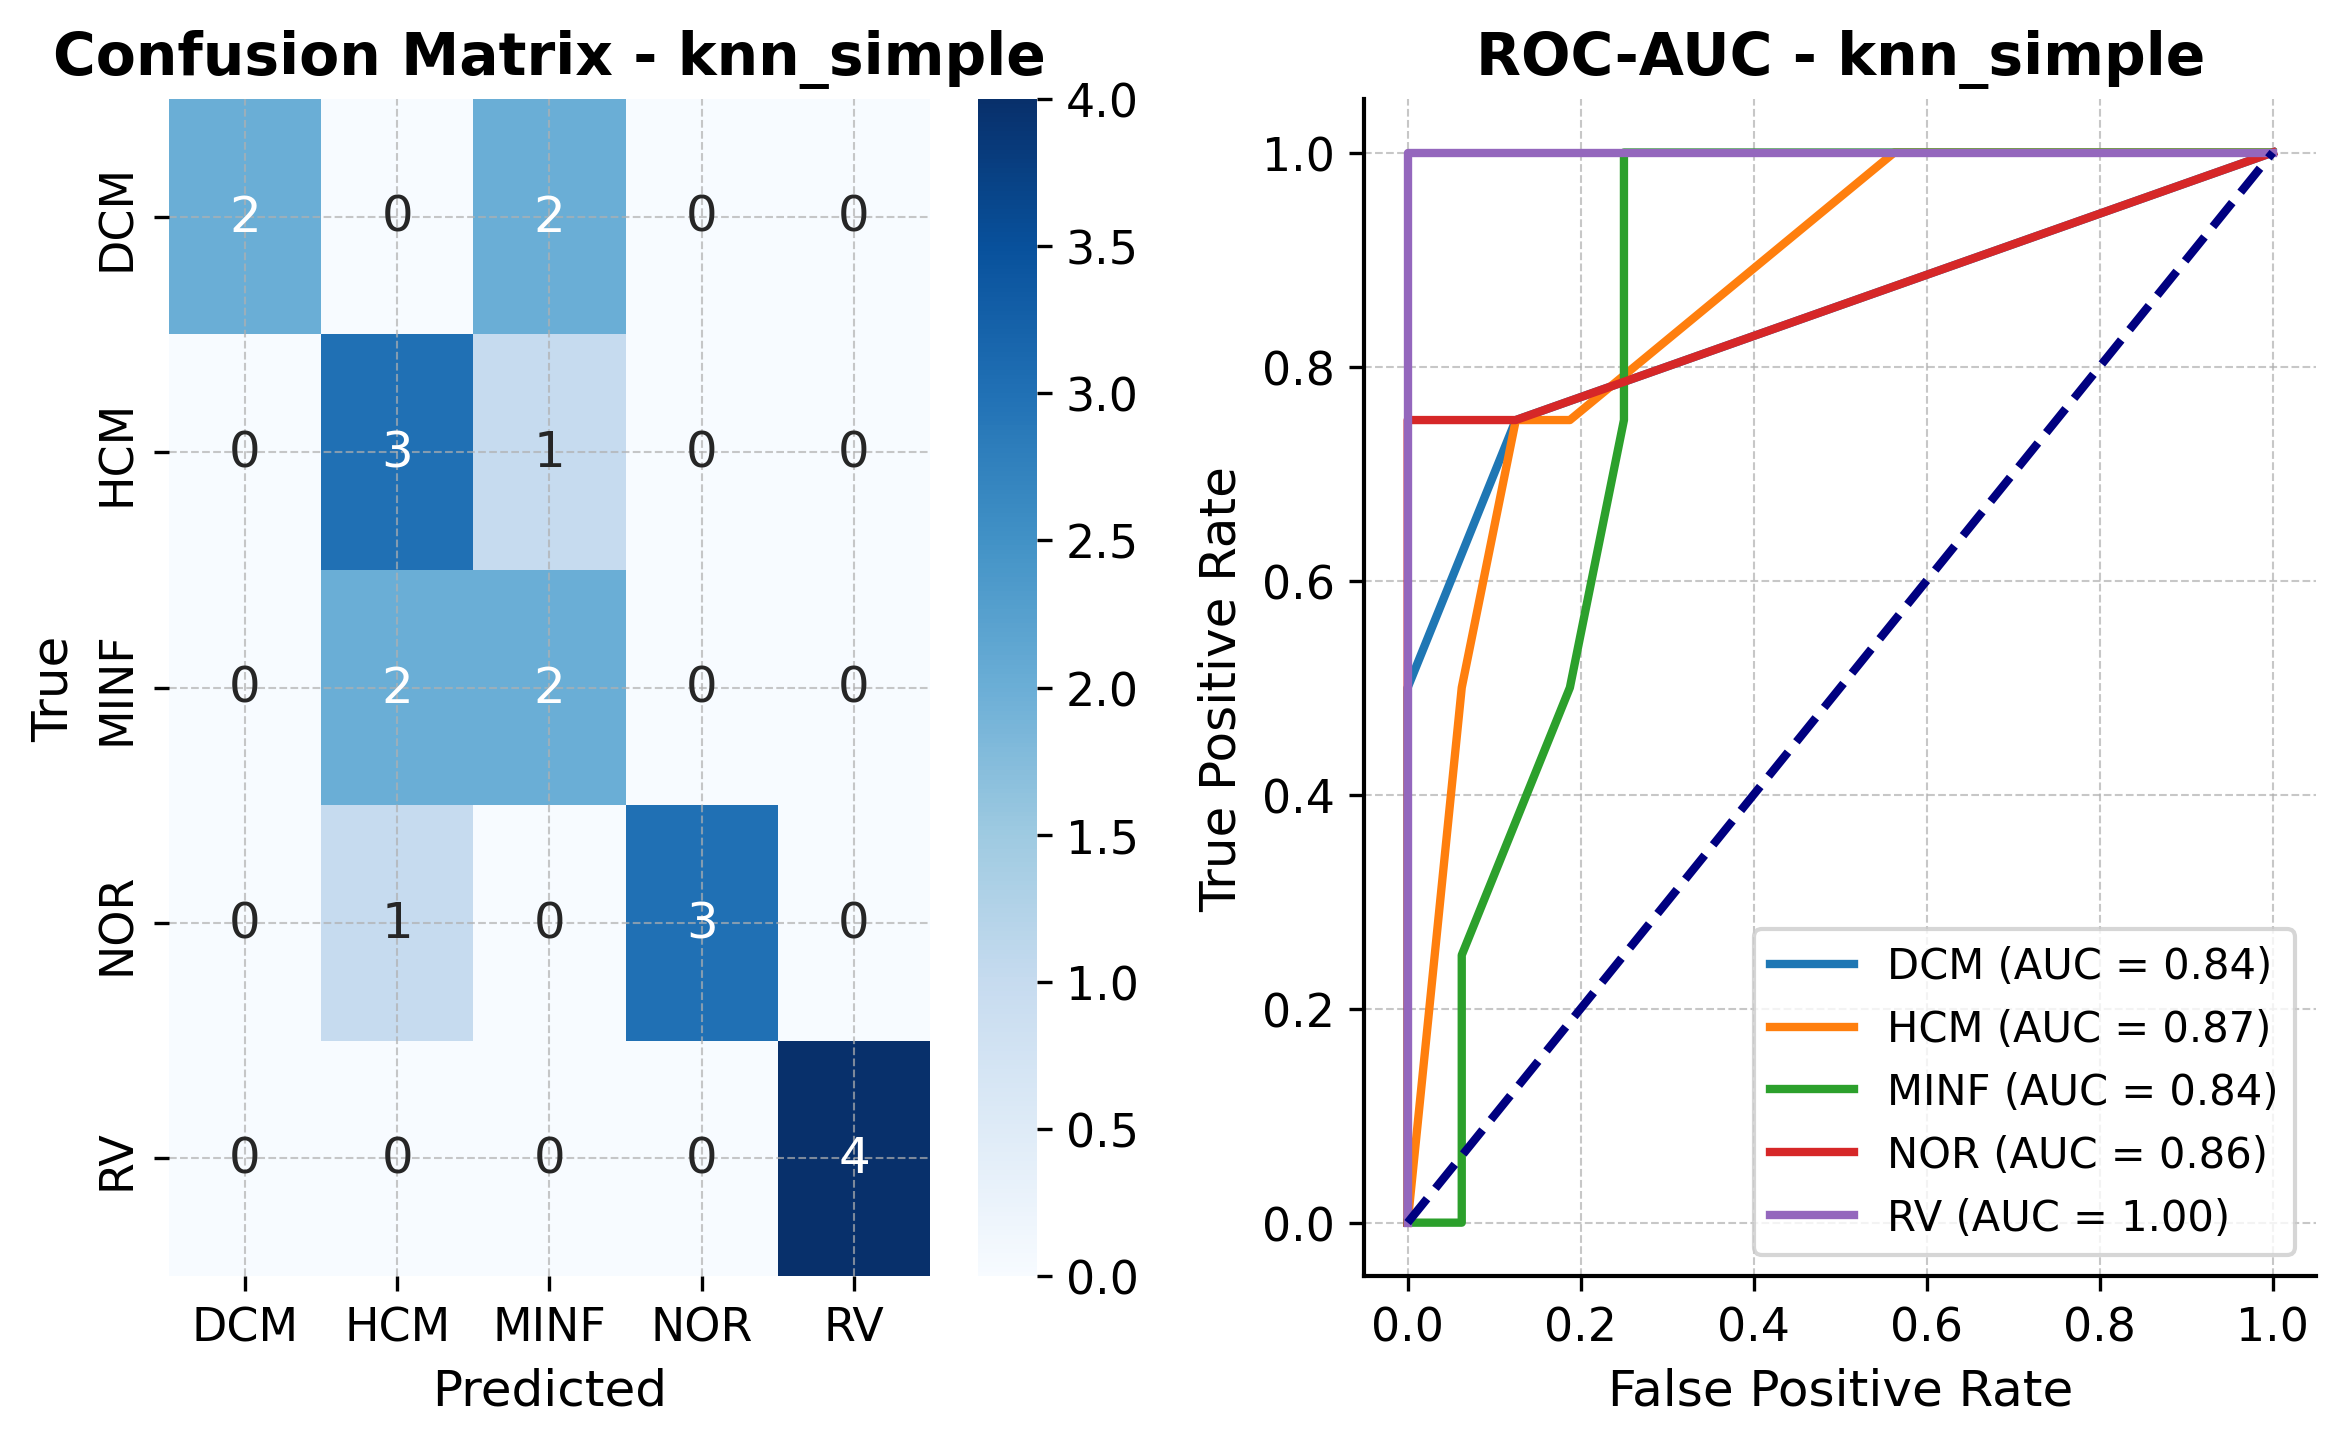
\includegraphics[width=0.99\textwidth]{../images/metrics/knn/knn_simple_metrics.png}
	\end{center}
	\caption{Confusion matrix and ROC curves for the k-Nearest Neighbors (KNN)
		model trained using the Simple Split strategy. DCM $=$ Dilated
		Cardiomyopathy, HCM $=$ Hypertrophic Cardiomyopathy, MINF $=$ Myocardial
		Infarction, NOR $=$ Normal, RV $=$ Right Ventricular abnormality.}
\end{figure}

\begin{figure}
	\begin{center}
		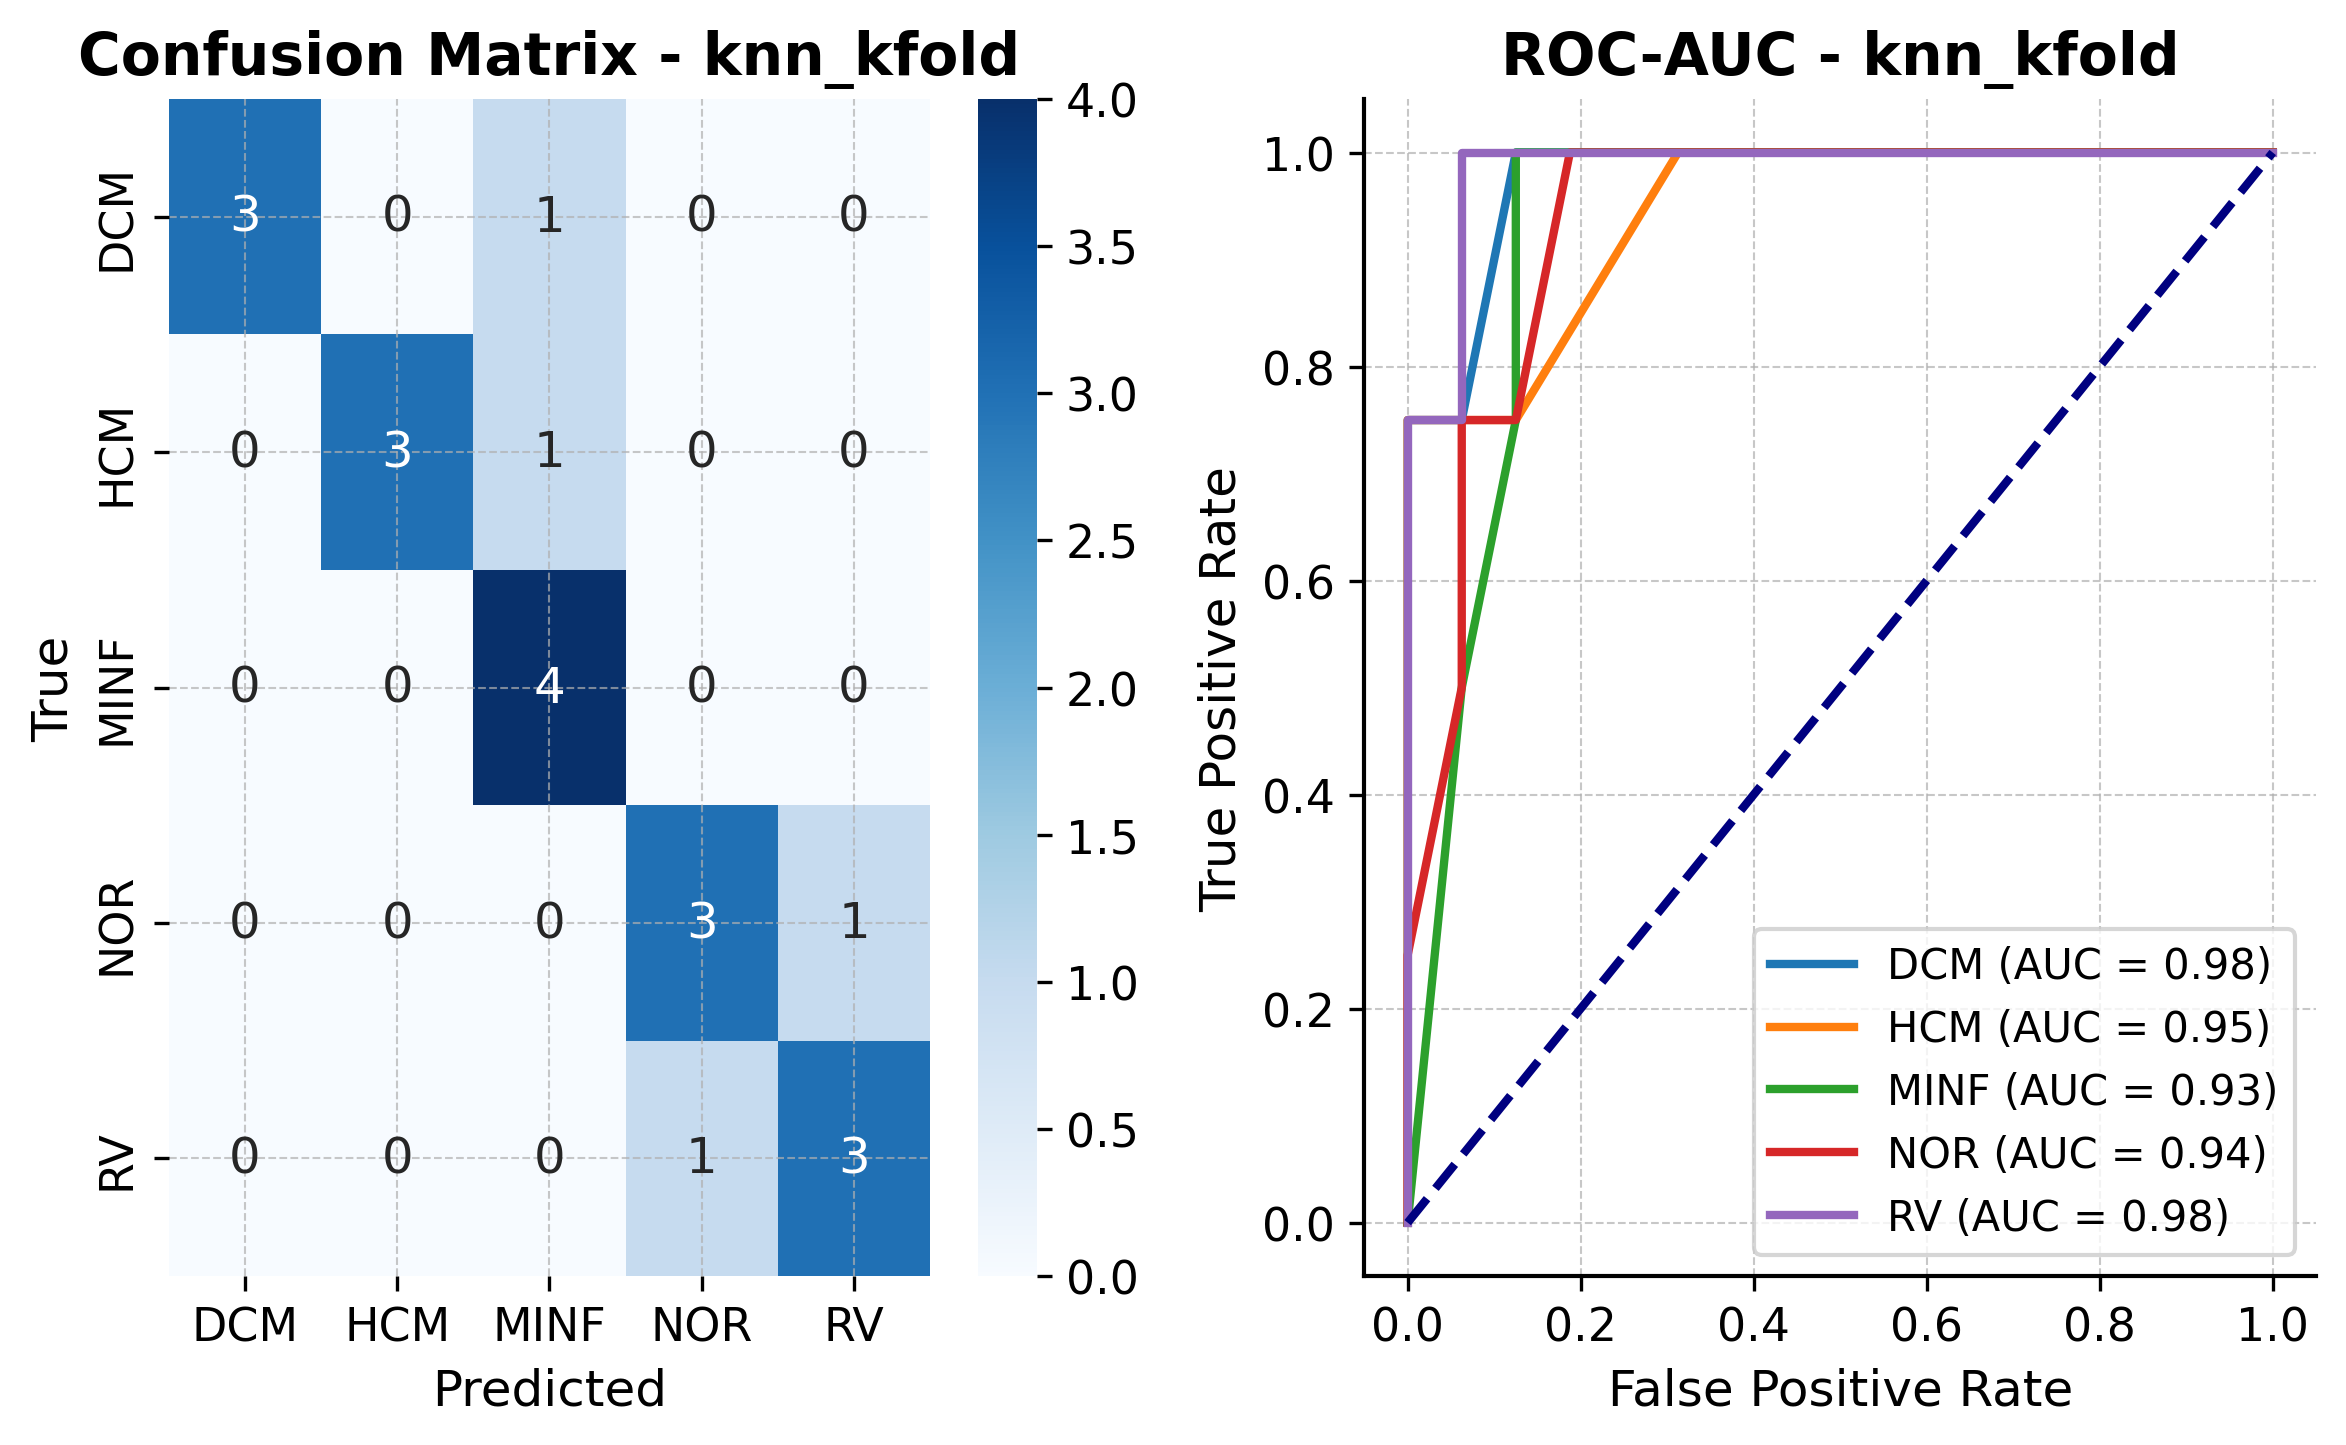
\includegraphics[width=0.99\textwidth]{../images/metrics/knn/knn_kfold_metrics.png}
	\end{center}
	\caption{Confusion matrix and ROC curves for the k-Nearest Neighbors (KNN)
		model trained with Stratified K-Fold cross-validation. DCM $=$ Dilated
		Cardiomyopathy, HCM $=$ Hypertrophic Cardiomyopathy, MINF $=$ Myocardial
		Infarction, NOR $=$ Normal, RV $=$ Right Ventricular abnormality.}
\end{figure}

\begin{figure}
	\begin{center}
		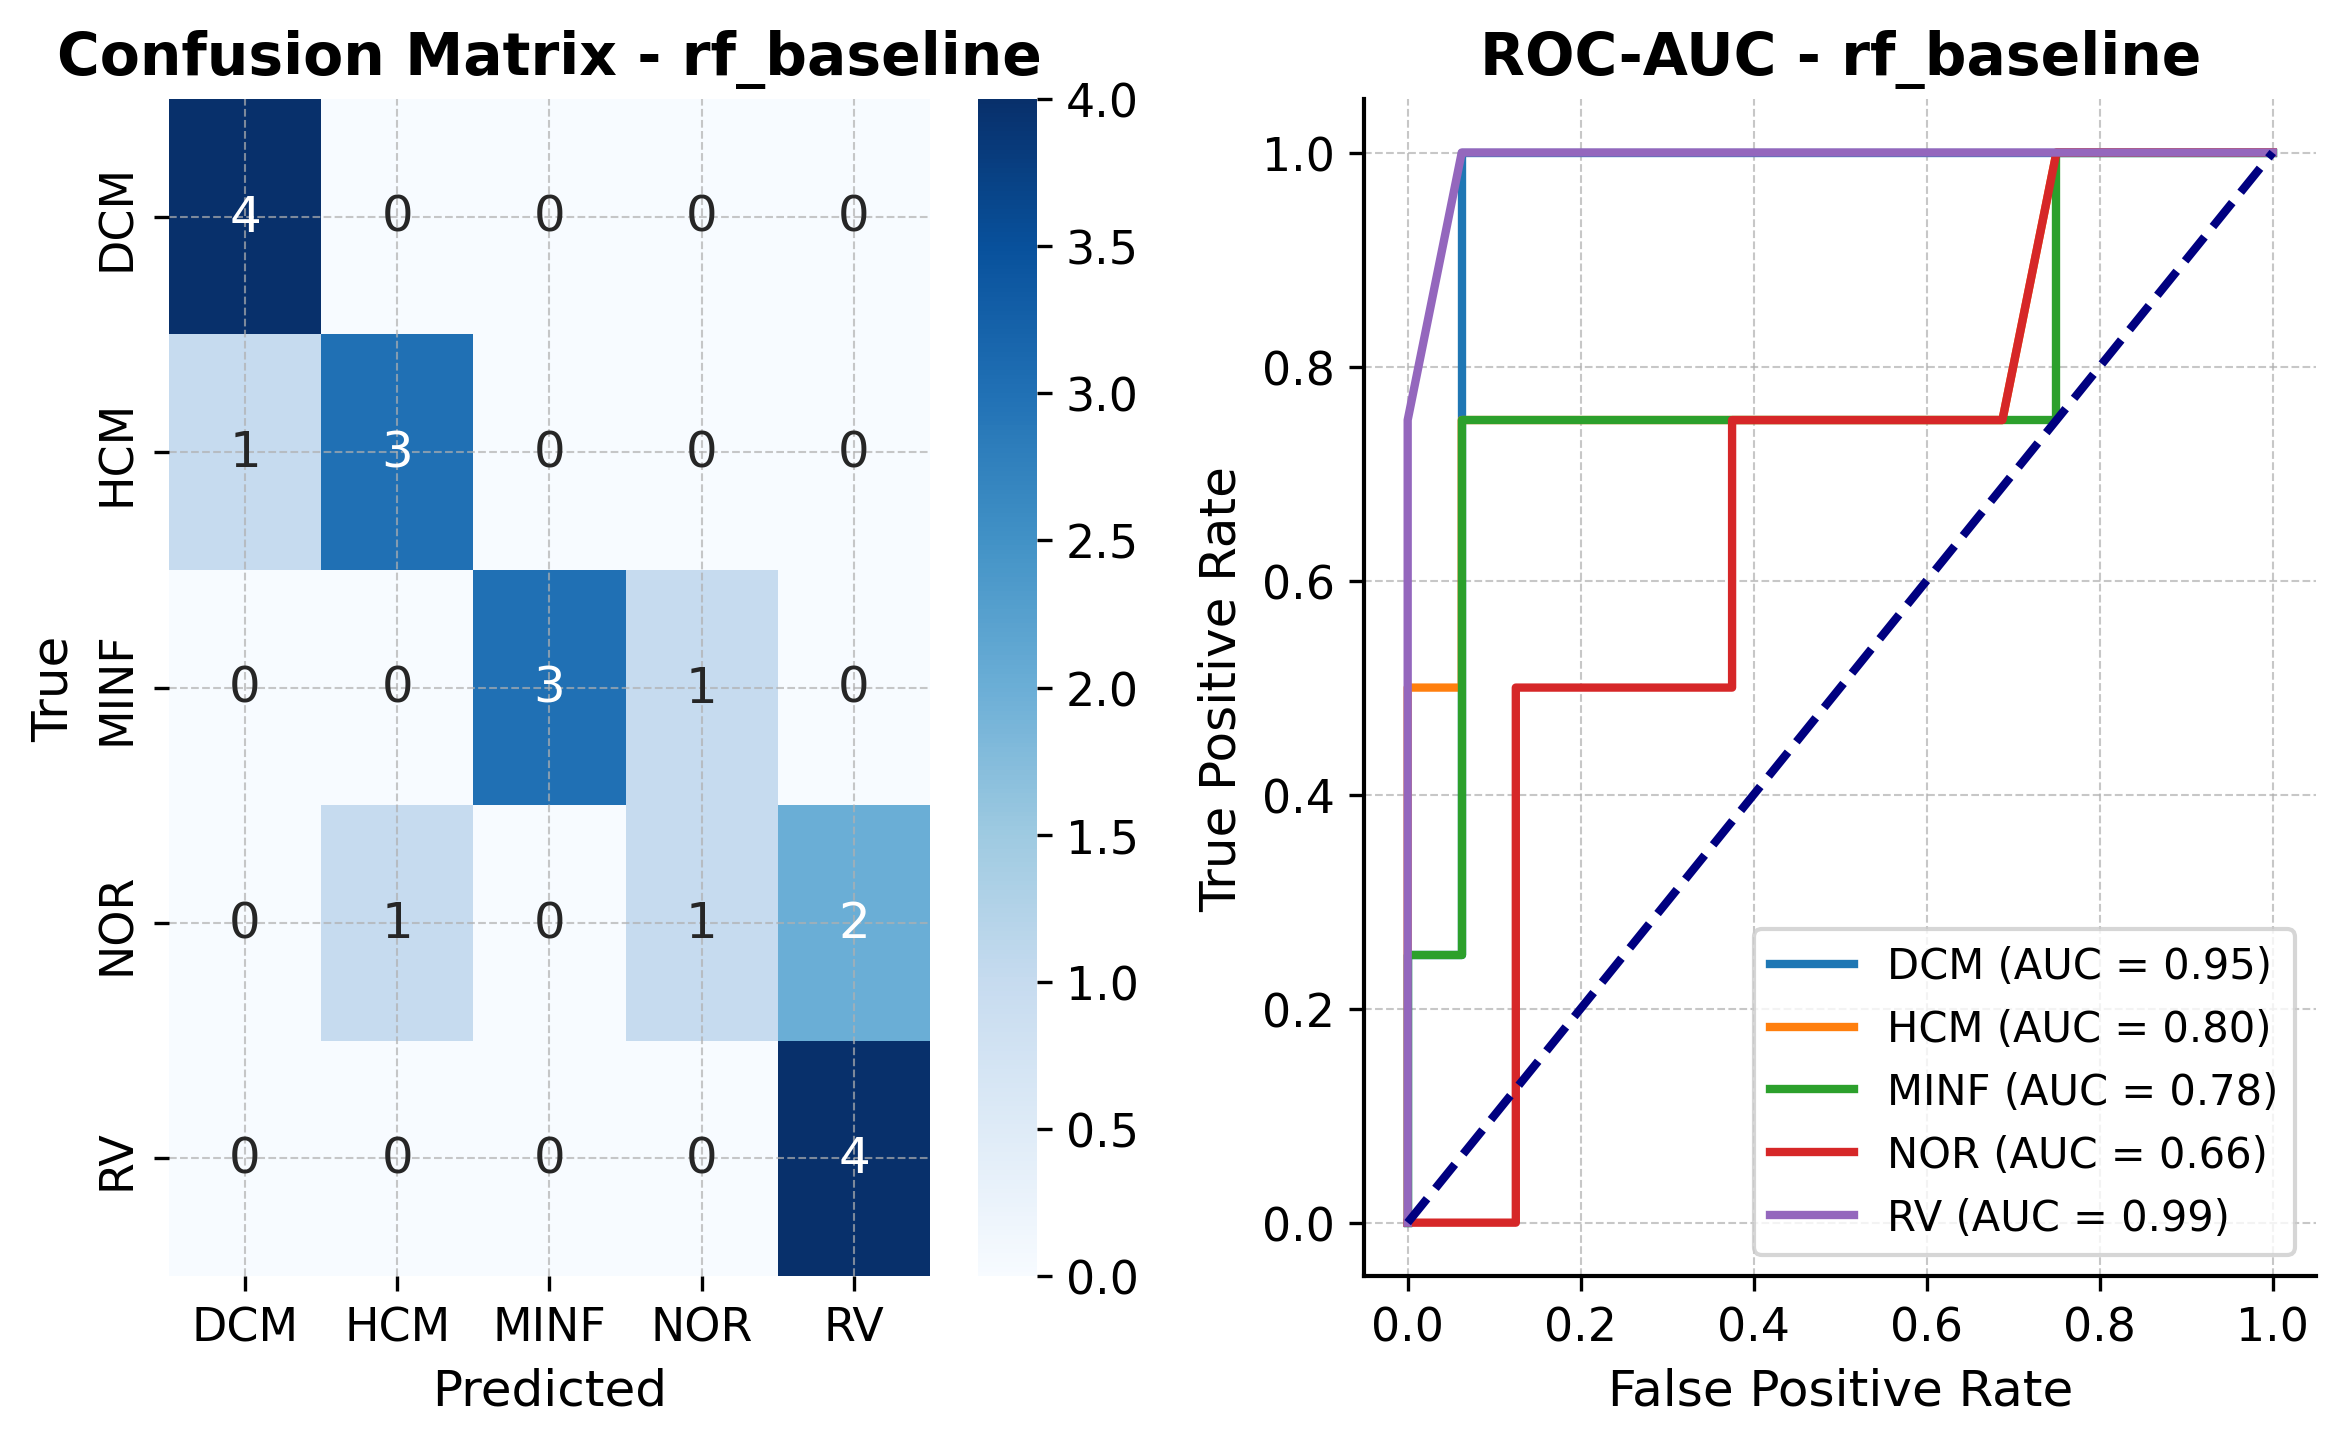
\includegraphics[width=0.99\textwidth]{../images/metrics/rf/rf_baseline_metrics.png}
	\end{center}
	\caption{Confusion matrix and ROC curves for the Random Forest (RF) model
		trained using no strategy. DCM $=$ Dilated Cardiomyopathy, HCM $=$
		Hypertrophic Cardiomyopathy, MINF $=$ Myocardial Infarction, NOR $=$ Normal, RV
		$=$ Right Ventricular abnormality.}
\end{figure}

\begin{figure}
	\begin{center}
		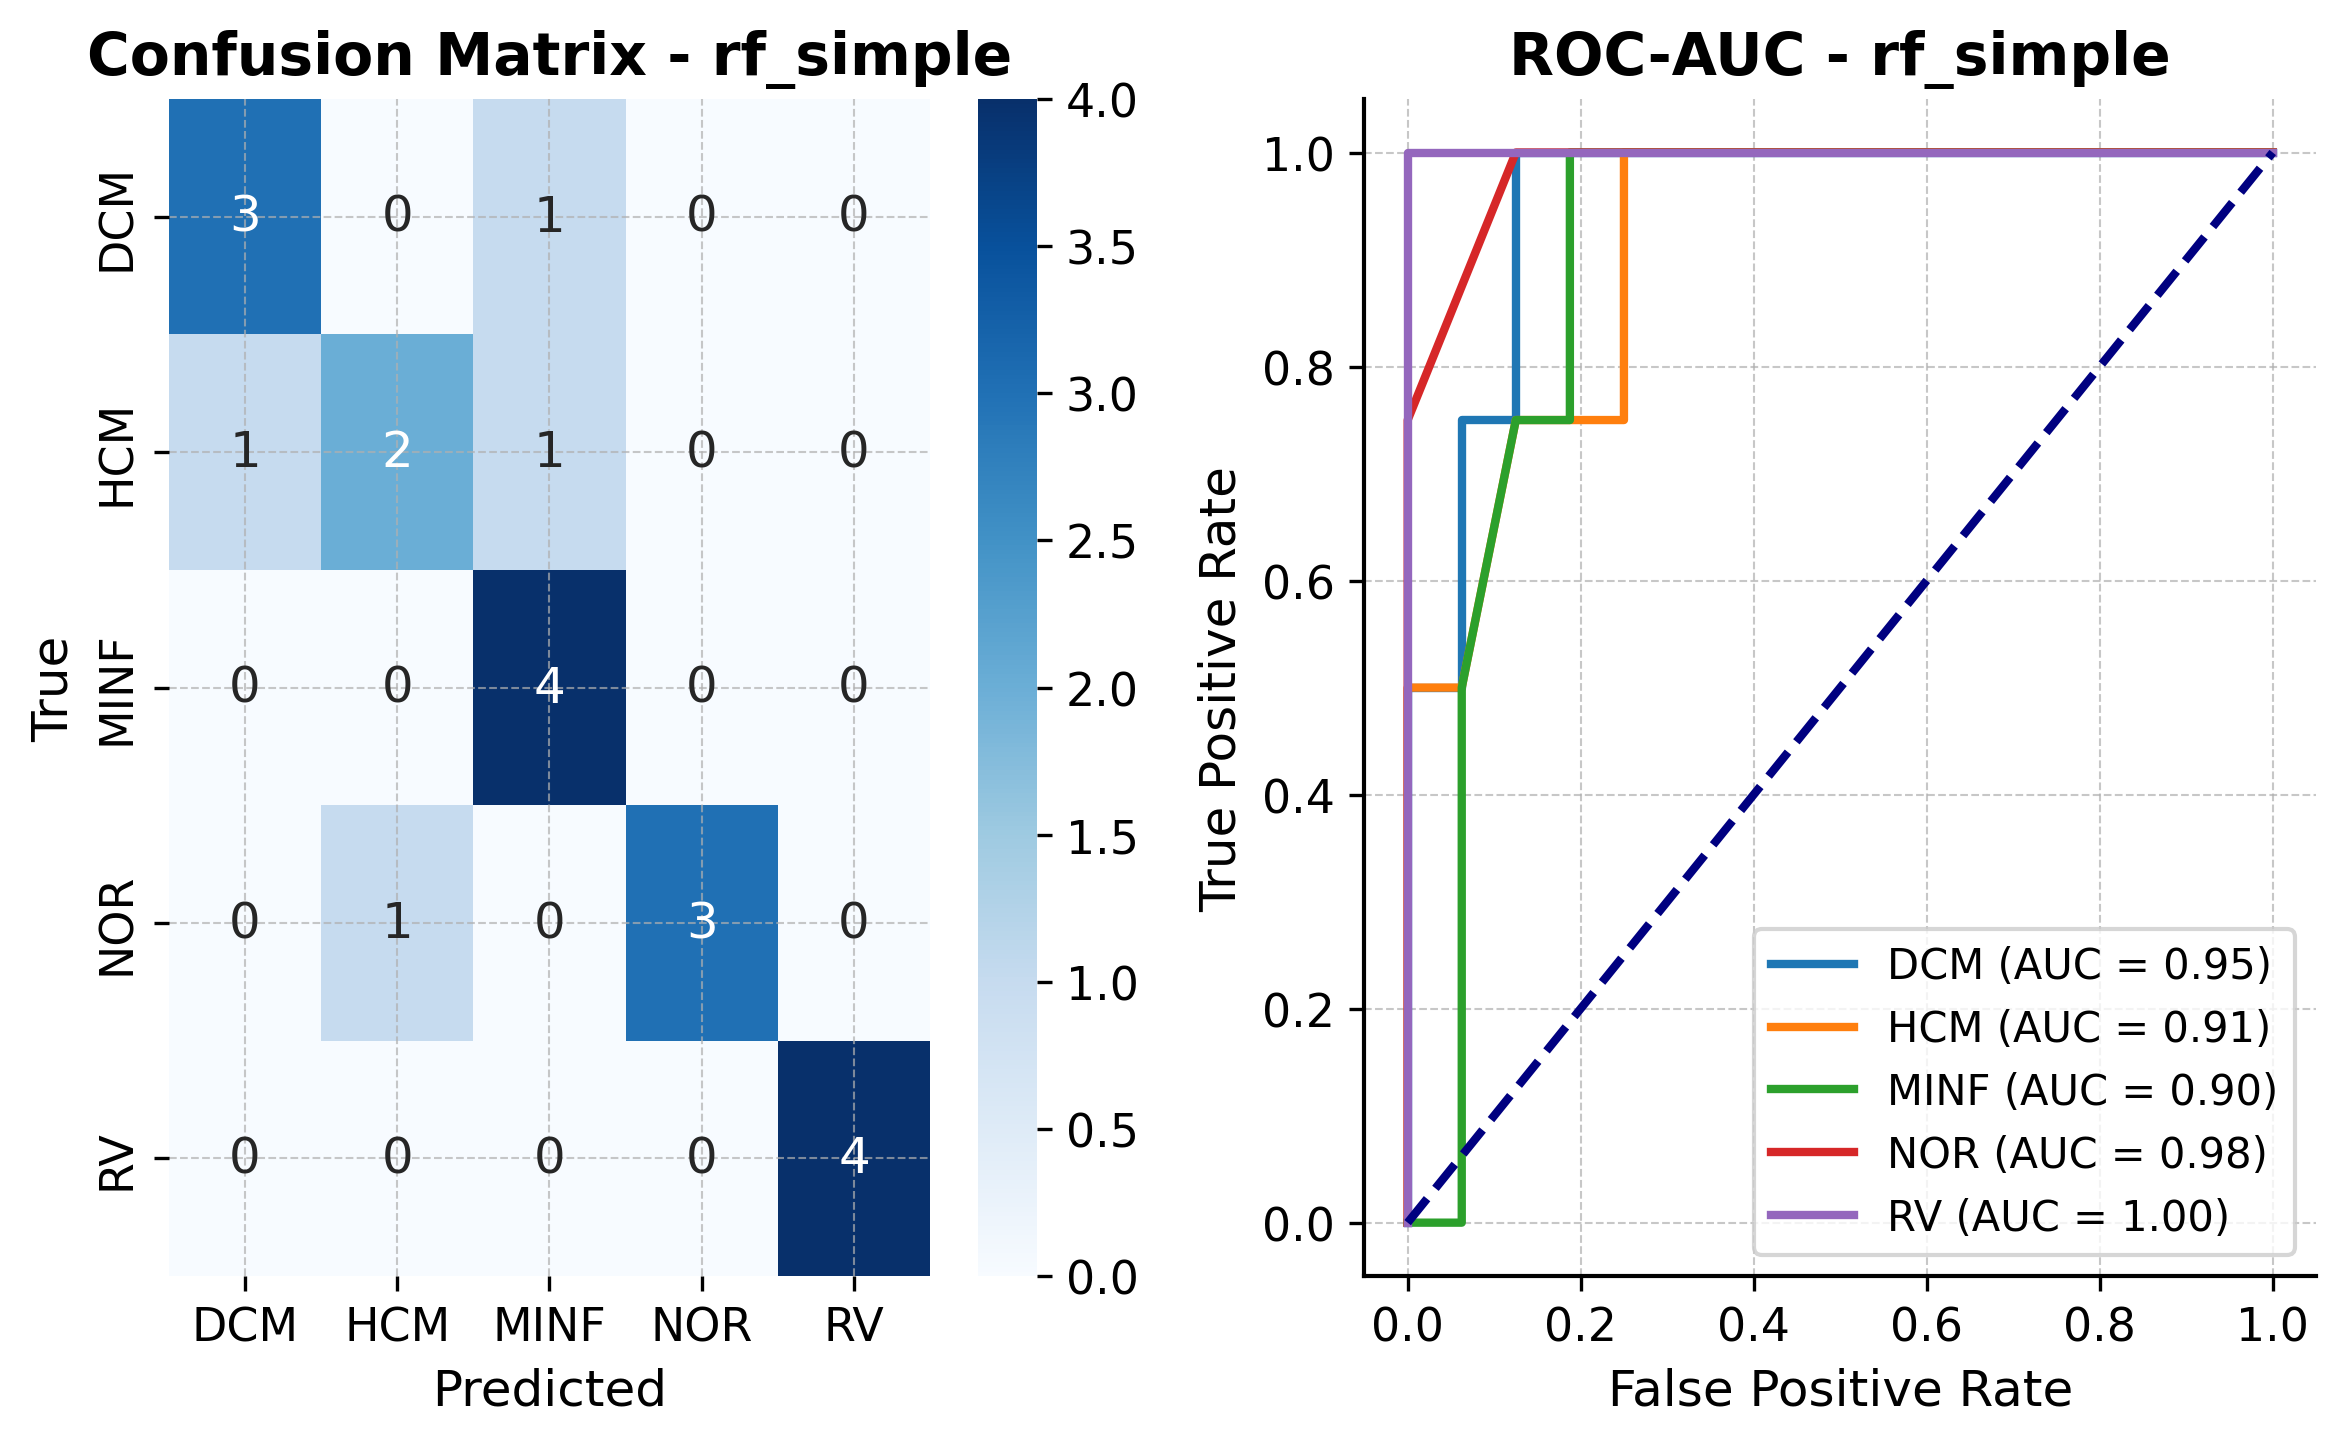
\includegraphics[width=0.99\textwidth]{../images/metrics/rf/rf_simple_metrics.png}
	\end{center}
	\caption{Confusion matrix and ROC curves for the Random Forest (RF) model
		trained using the Simple Split strategy. DCM $=$ Dilated Cardiomyopathy, HCM
		$=$ Hypertrophic Cardiomyopathy, MINF $=$ Myocardial Infarction, NOR $=$
		Normal, RV $=$ Right Ventricular abnormality.}
\end{figure}

\begin{figure}
	\begin{center}
		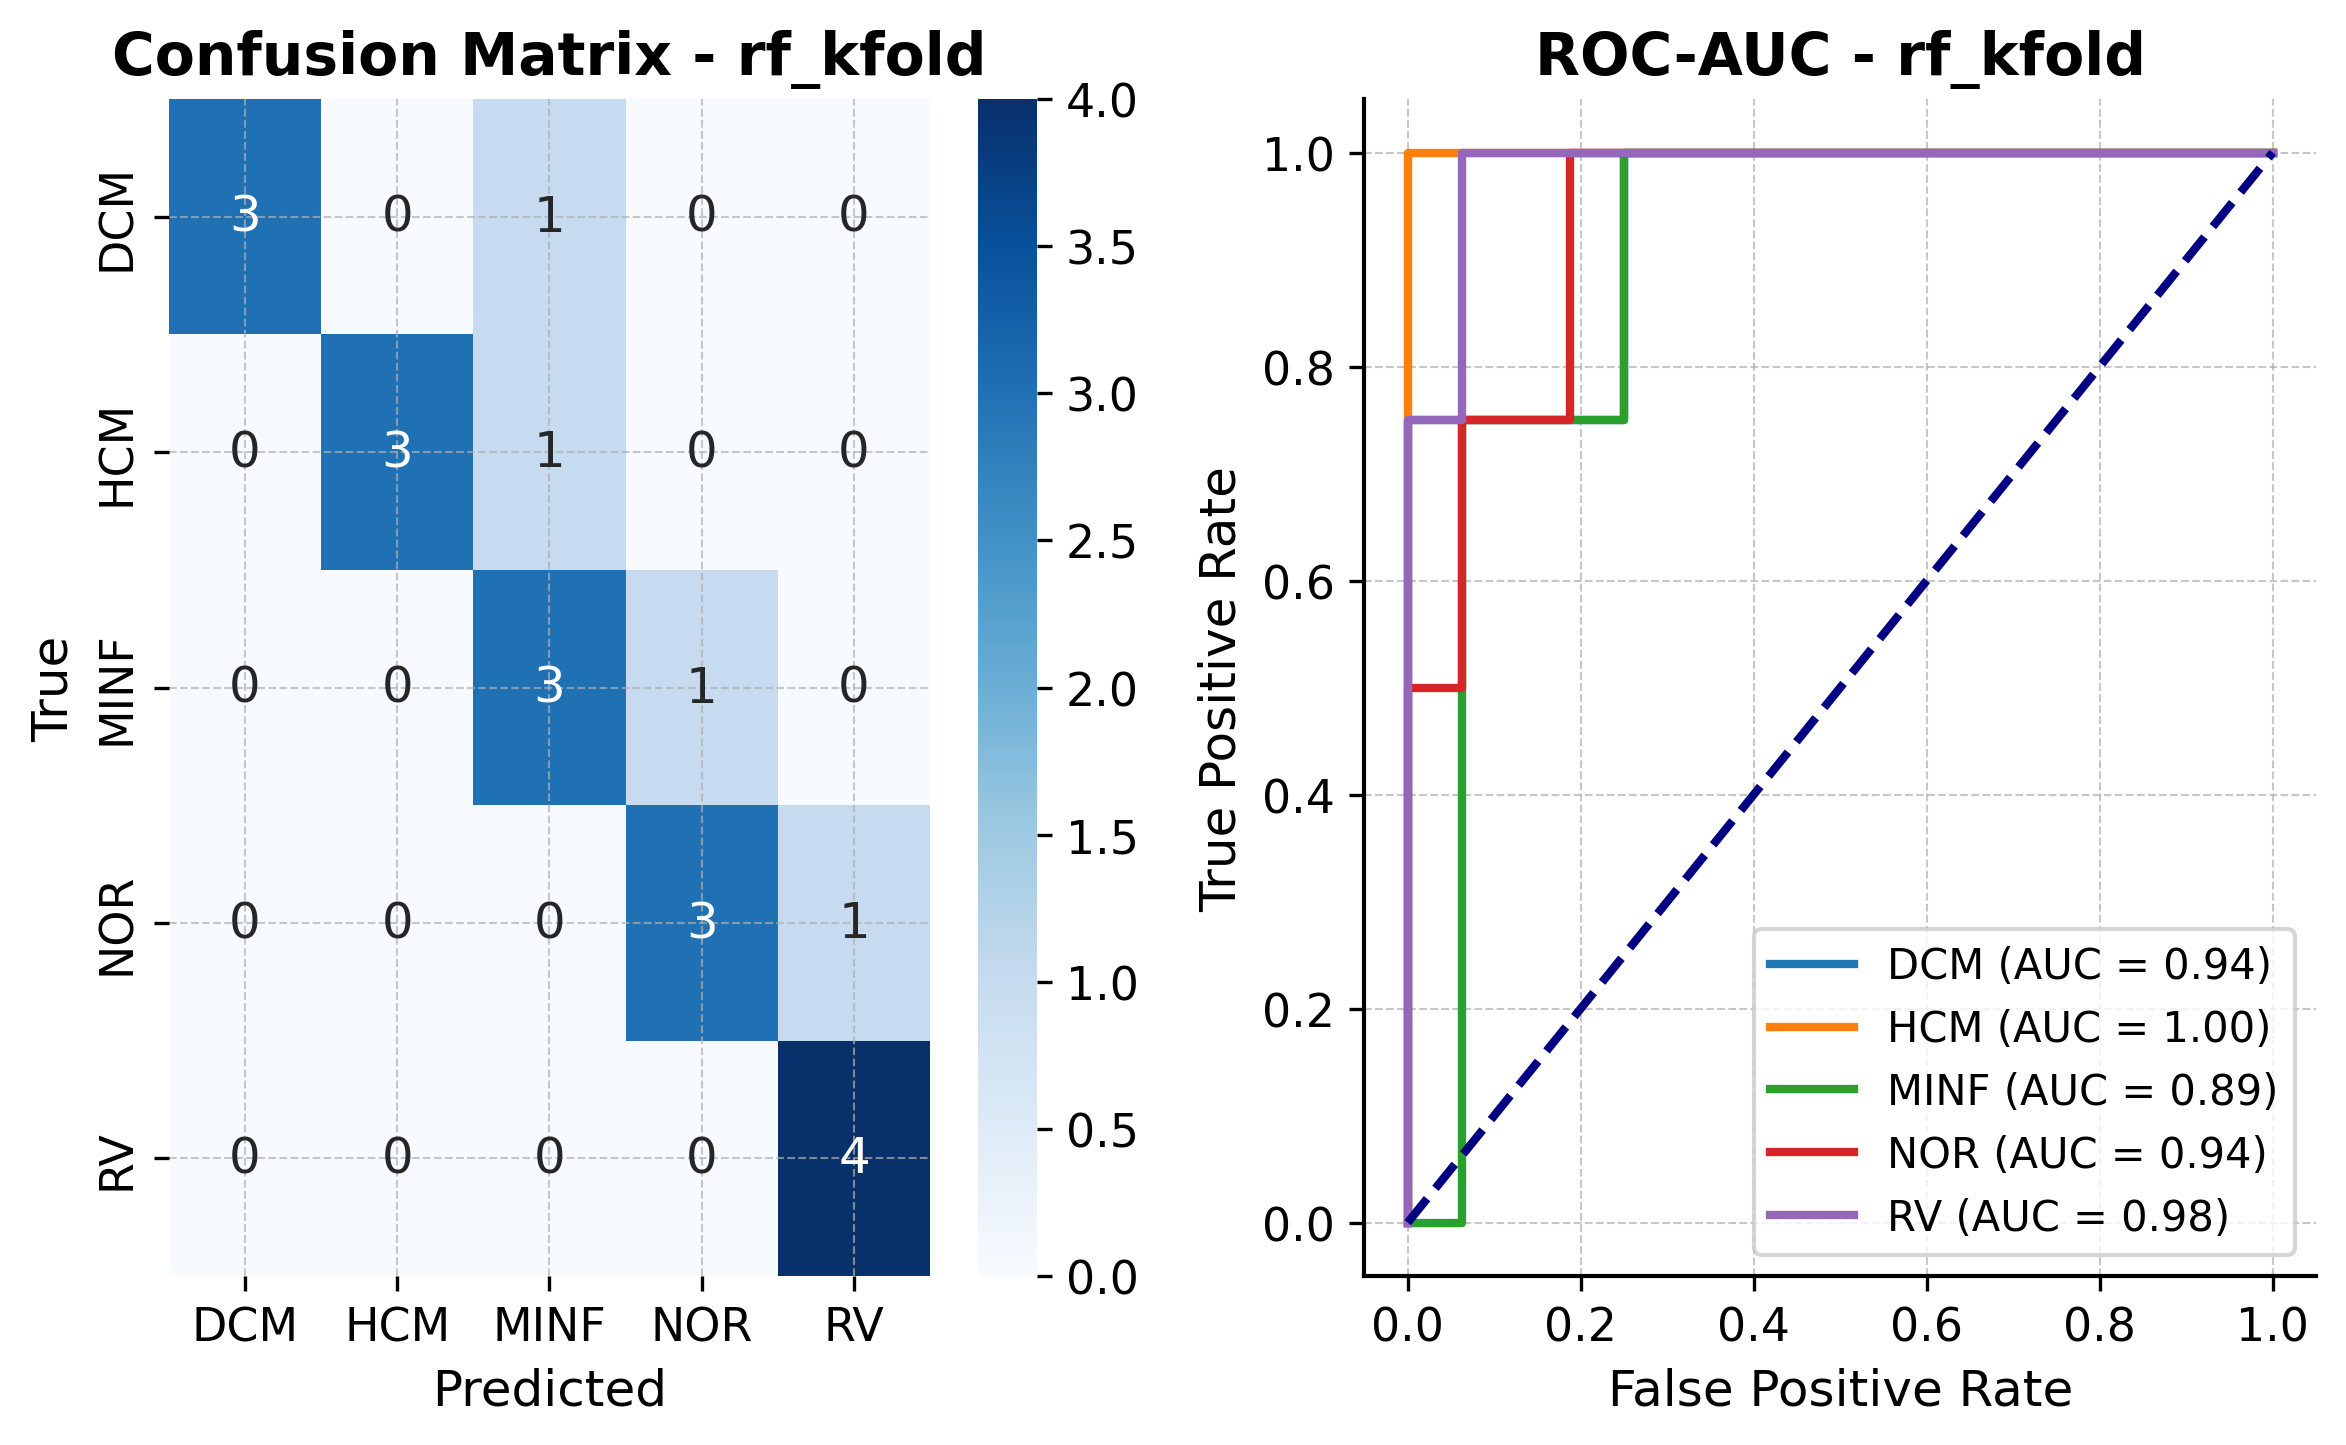
\includegraphics[width=0.99\textwidth]{../images/metrics/rf/rf_kfold_metrics.png}
	\end{center}
	\caption{Confusion matrix and ROC curves for the Random Forest (RF) model
		trained with Stratified K-Fold cross-validation. DCM $=$ Dilated
		Cardiomyopathy, HCM $=$ Hypertrophic Cardiomyopathy, MINF $=$ Myocardial
		Infarction, NOR $=$ Normal, RV $=$ Right Ventricular abnormality.}
\end{figure}

\begin{figure}
	\begin{center}
		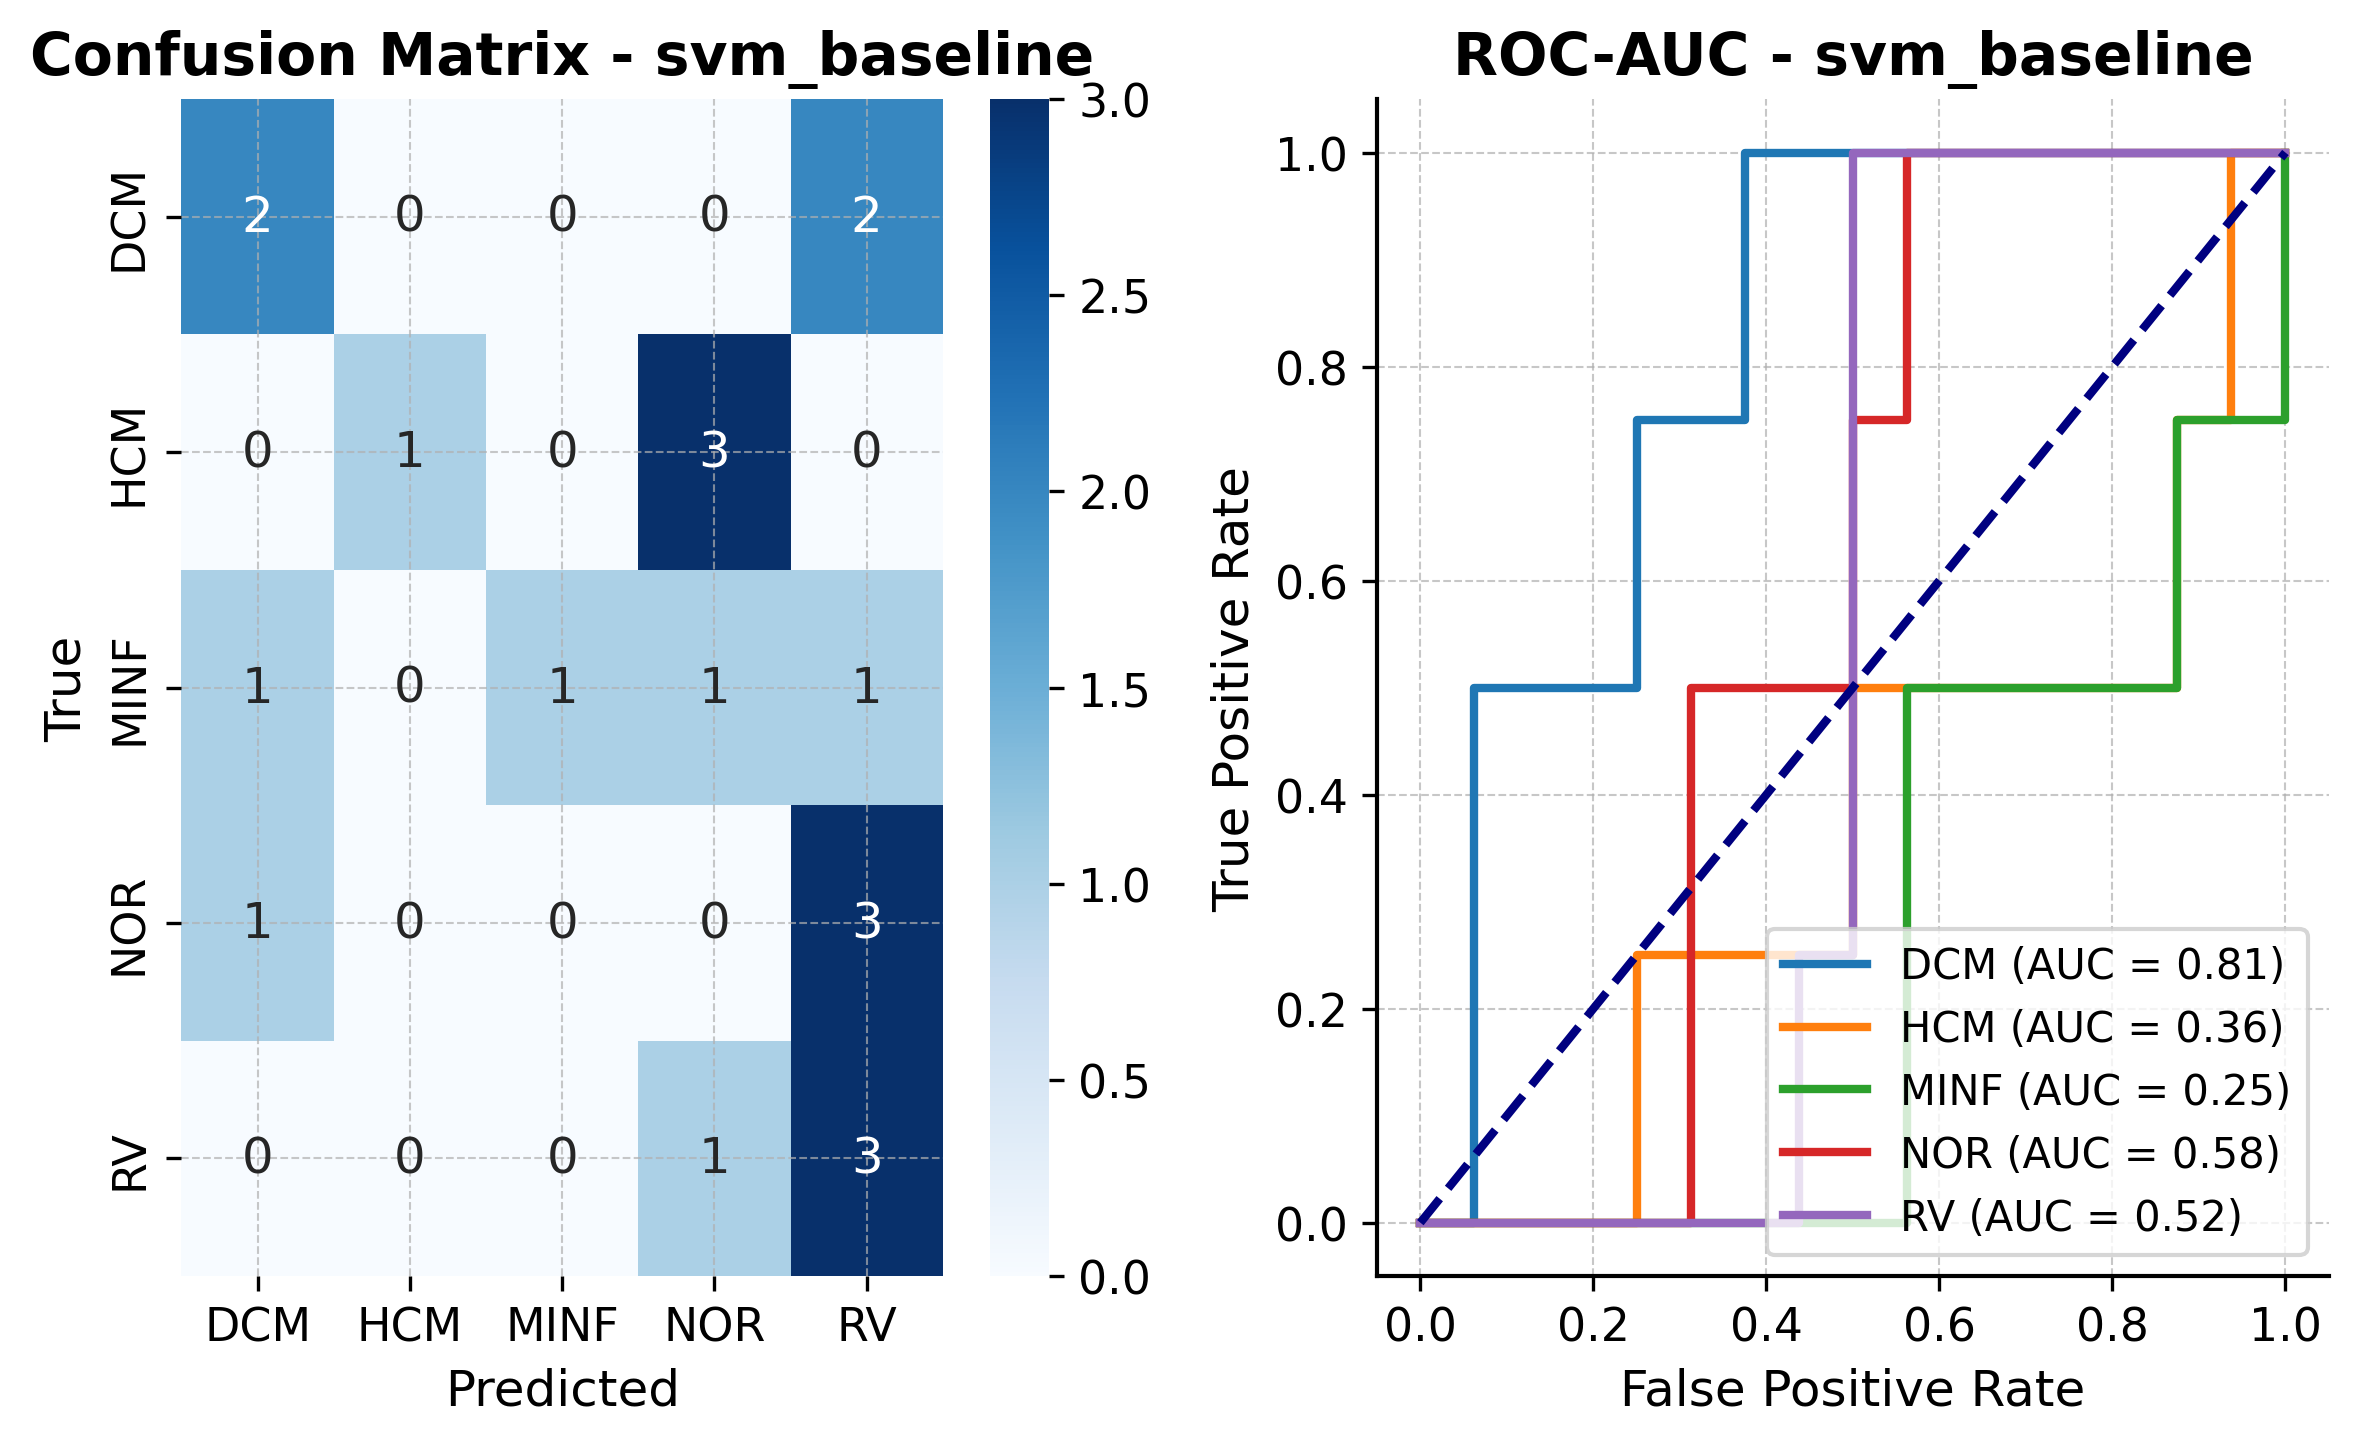
\includegraphics[width=0.99\textwidth]{../images/metrics/svm/svm_baseline_metrics.png}
	\end{center}
	\caption{Confusion matrix and ROC curves for the Support Vector Machine (SVM)
		model trained using no strategy. DCM $=$ Dilated Cardiomyopathy, HCM $=$
		Hypertrophic Cardiomyopathy, MINF $=$ Myocardial Infarction, NOR $=$ Normal, RV
		$=$ Right Ventricular abnormality.}
\end{figure}

\begin{figure}
	\begin{center}
		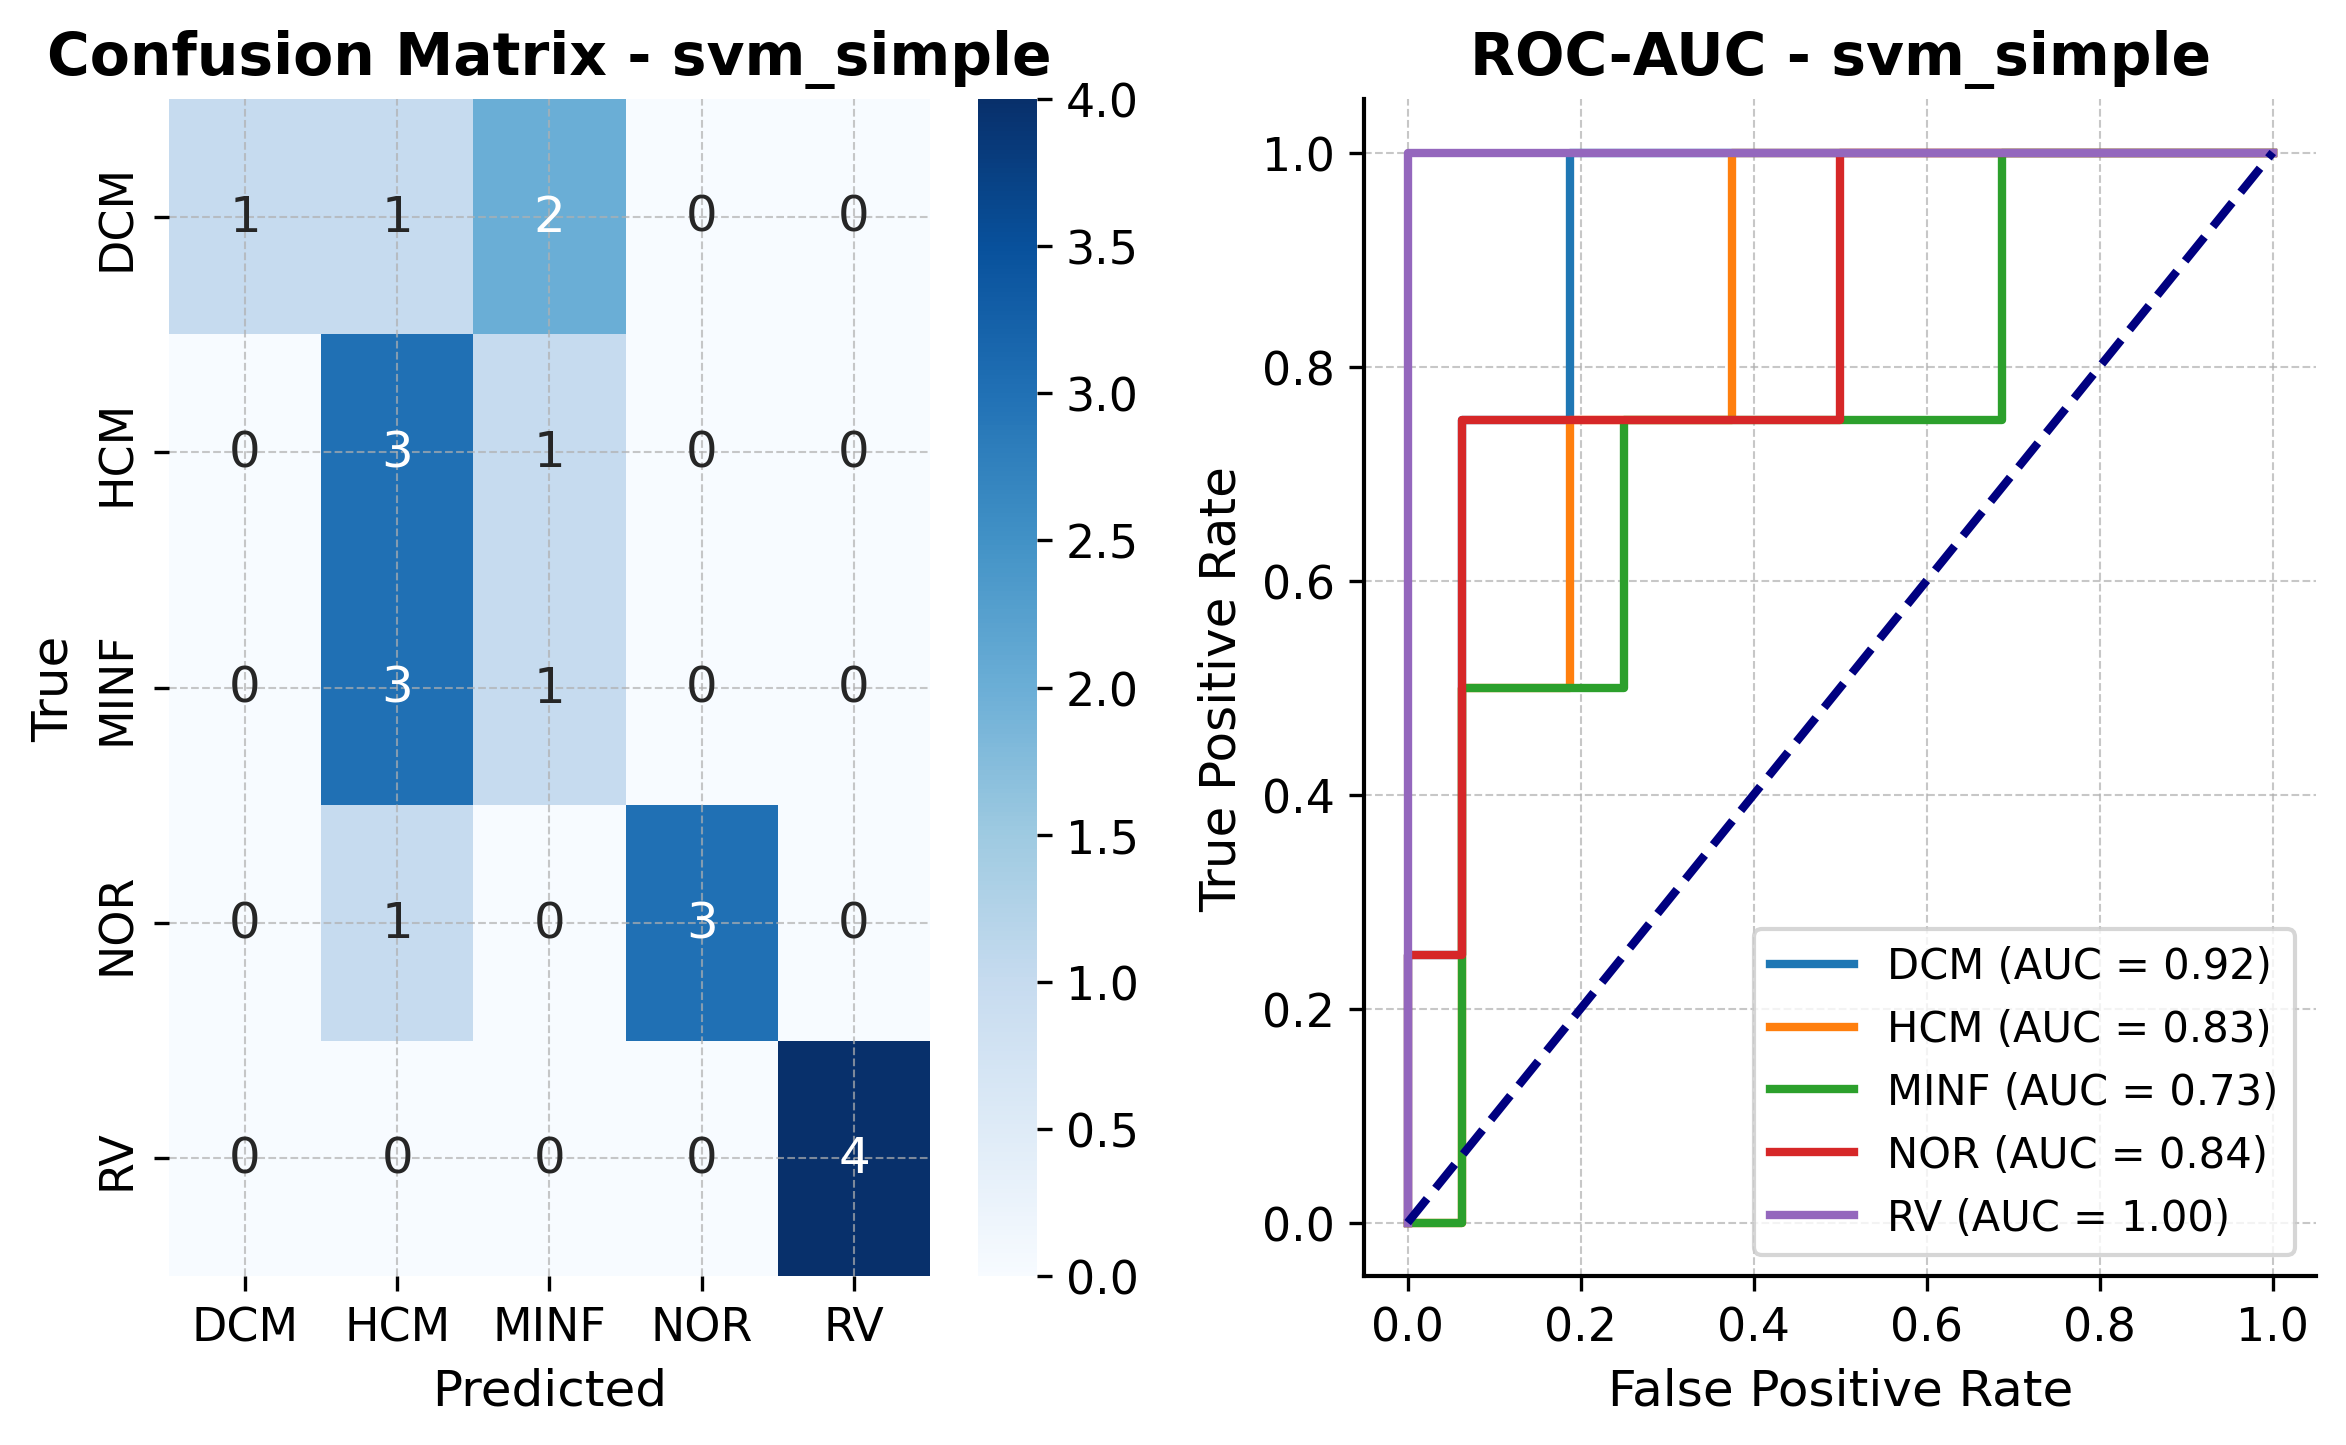
\includegraphics[width=0.99\textwidth]{../images/metrics/svm/svm_simple_metrics.png}
	\end{center}
	\caption{Confusion matrix and ROC curves for the Support Vector Machine (SVM)
		model trained using the Simple Split strategy. DCM $=$ Dilated
		Cardiomyopathy, HCM $=$ Hypertrophic Cardiomyopathy, MINF $=$ Myocardial
		Infarction, NOR $=$ Normal, RV $=$ Right Ventricular abnormality.}
\end{figure}

\begin{figure}
	\begin{center}
		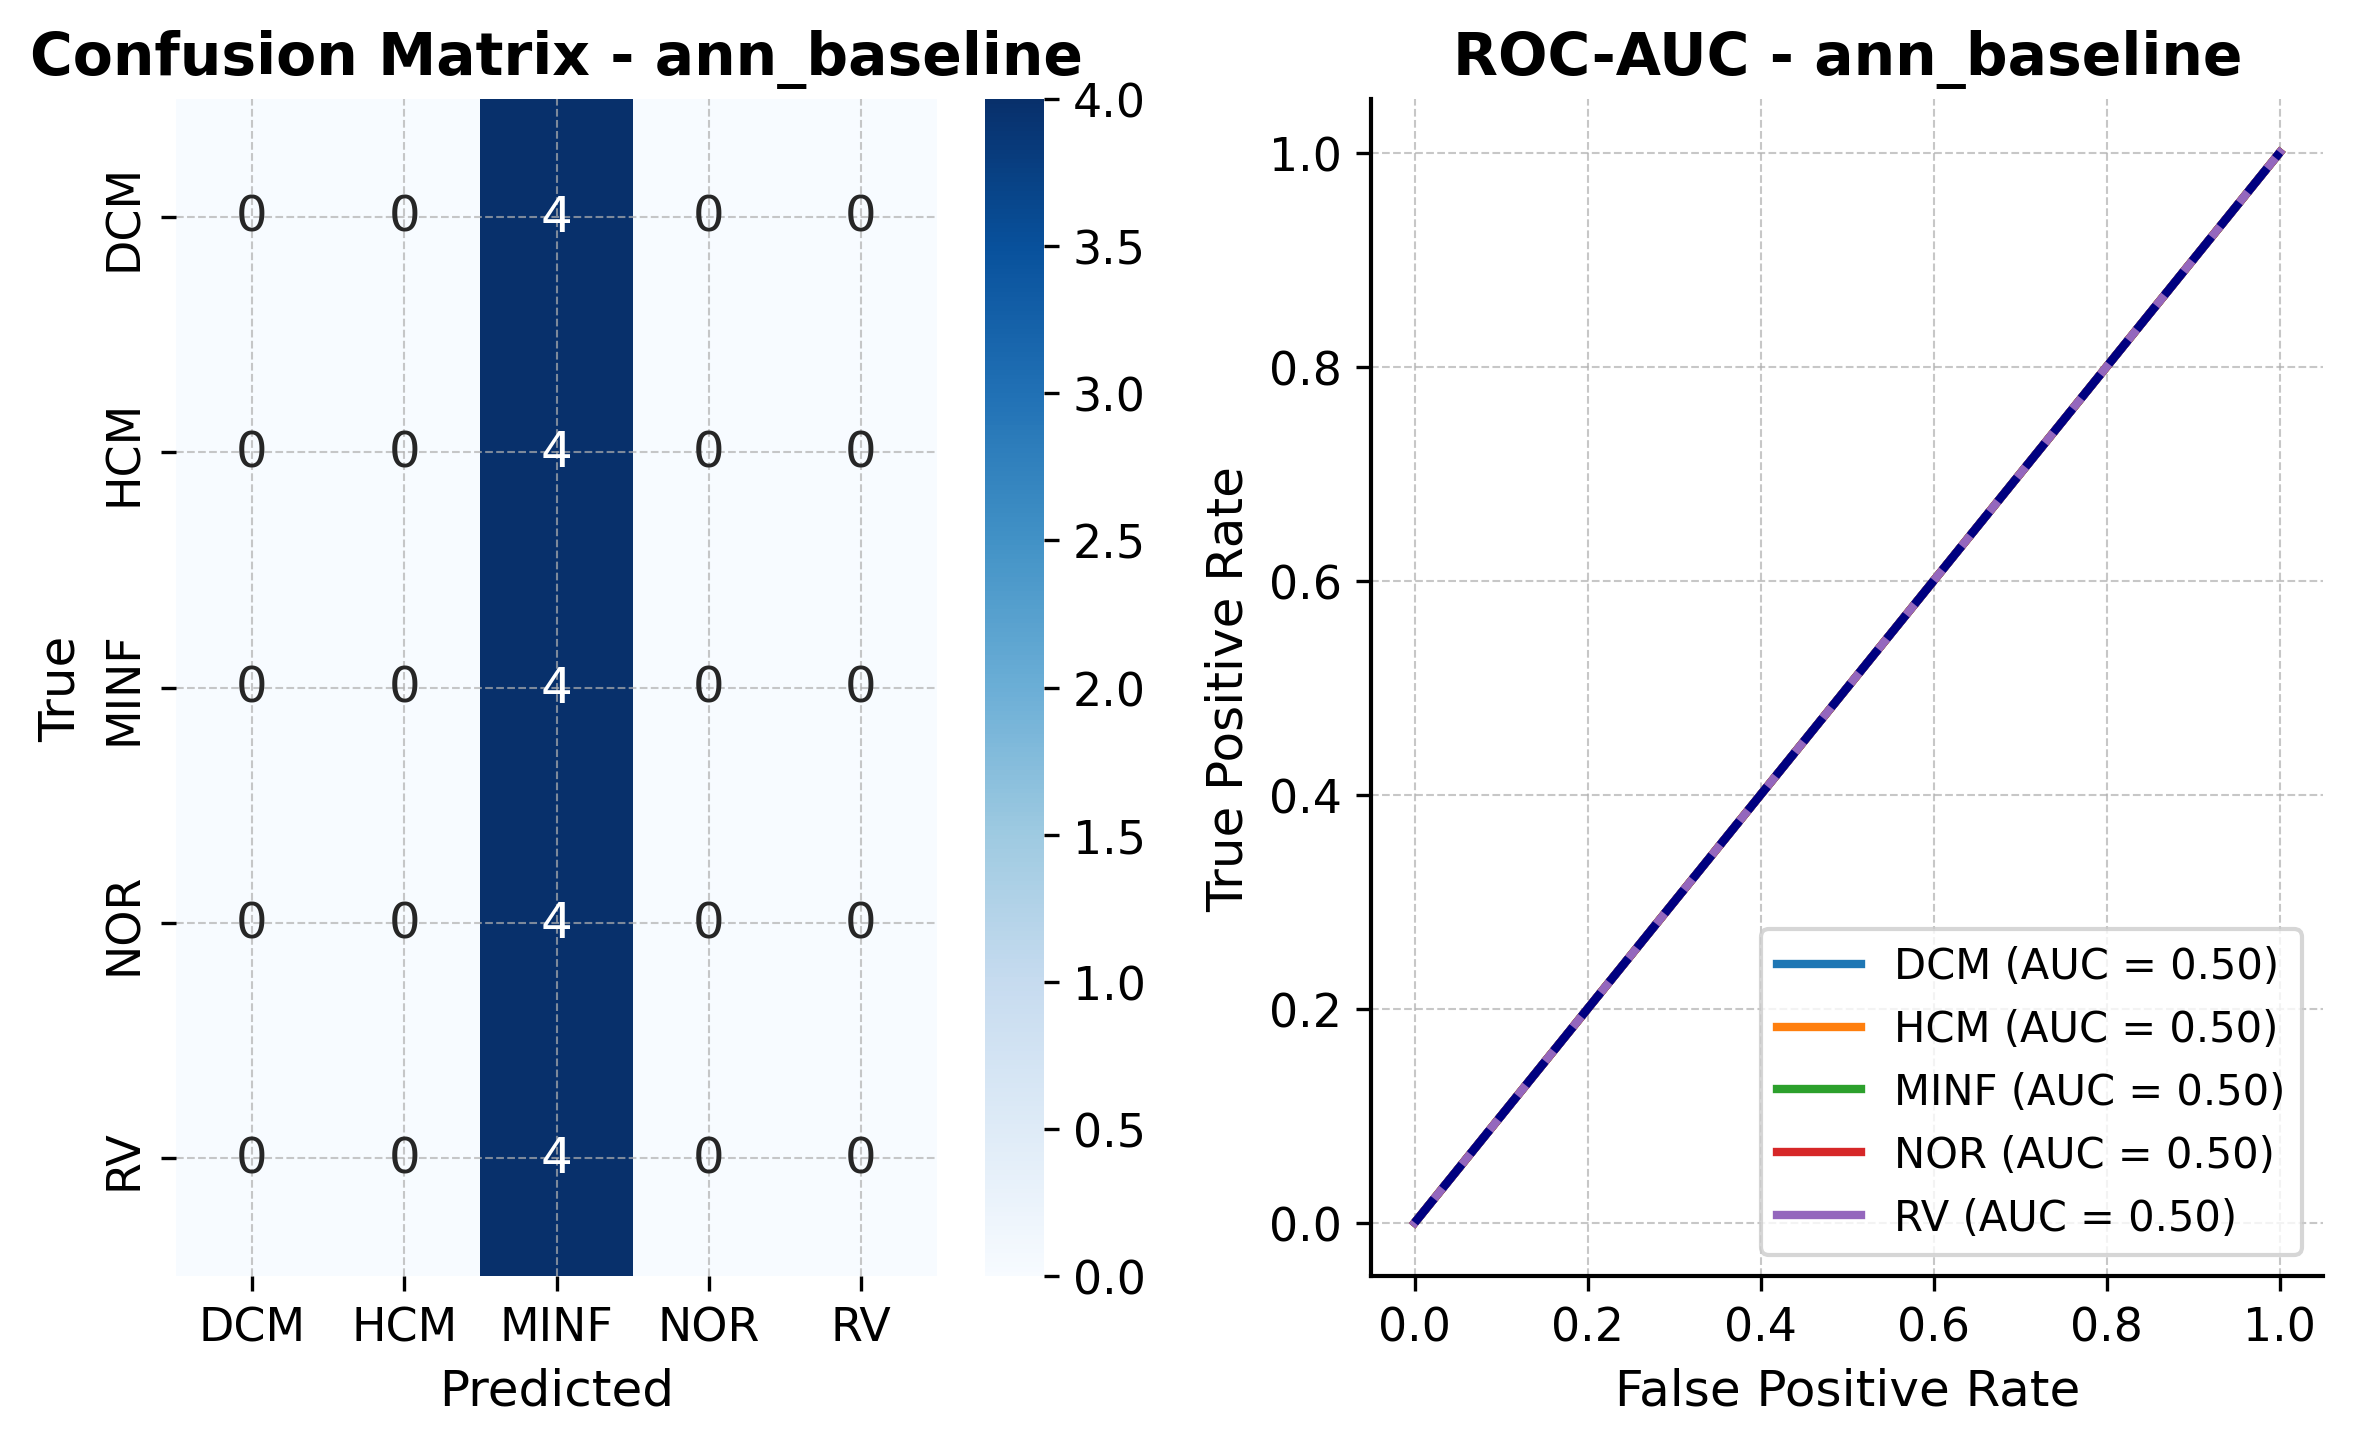
\includegraphics[width=0.99\textwidth]{../images/metrics/ann/ann_baseline_metrics.png}
	\end{center}
	\caption{Confusion matrix and ROC curves for the Artificial Neural Network
		(ANN) model trained using no strategy. DCM $=$ Dilated Cardiomyopathy, HCM
		$=$ Hypertrophic Cardiomyopathy, MINF $=$ Myocardial Infarction, NOR $=$
		Normal, RV $=$ Right Ventricular abnormality.}
\end{figure}

\begin{figure}
	\begin{center}
		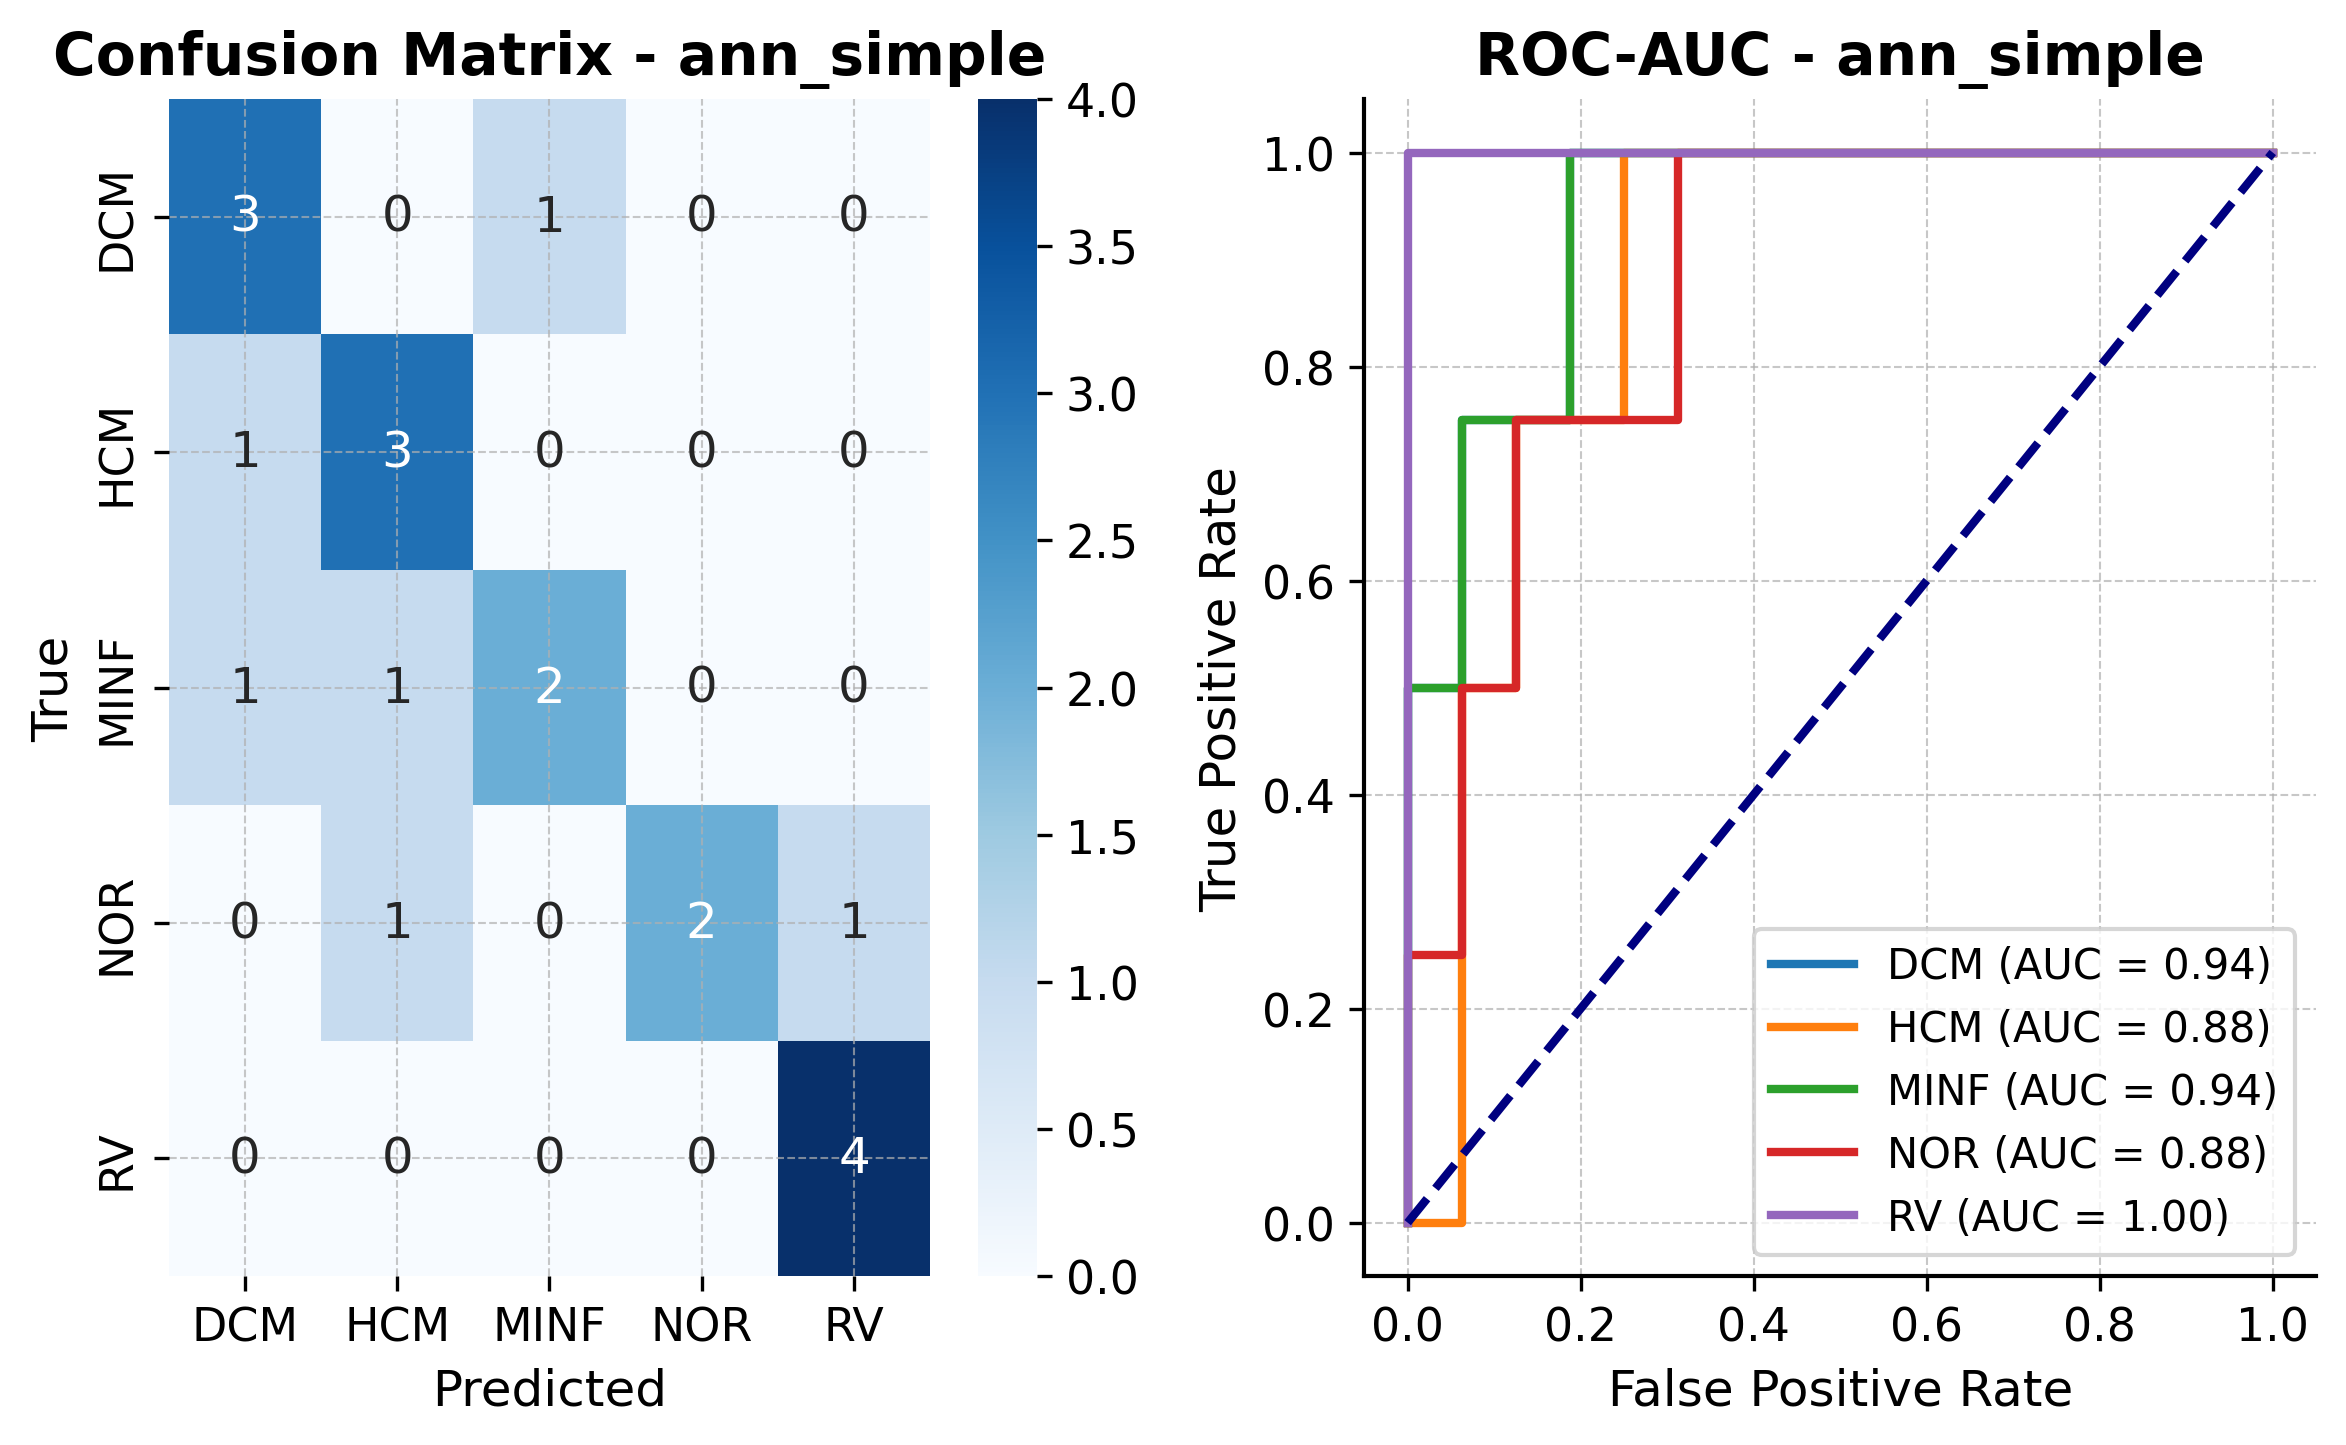
\includegraphics[width=0.99\textwidth]{../images/metrics/ann/ann_simple_metrics.png}
	\end{center}
	\caption{Confusion matrix and ROC curves for the Artificial Neural Network
		(ANN) model trained using the Simple Split strategy. DCM $=$ Dilated
		Cardiomyopathy, HCM $=$ Hypertrophic Cardiomyopathy, MINF $=$ Myocardial
		Infarction, NOR $=$ Normal, RV $=$ Right Ventricular abnormality.}
\end{figure}

\begin{figure}
	\begin{center}
		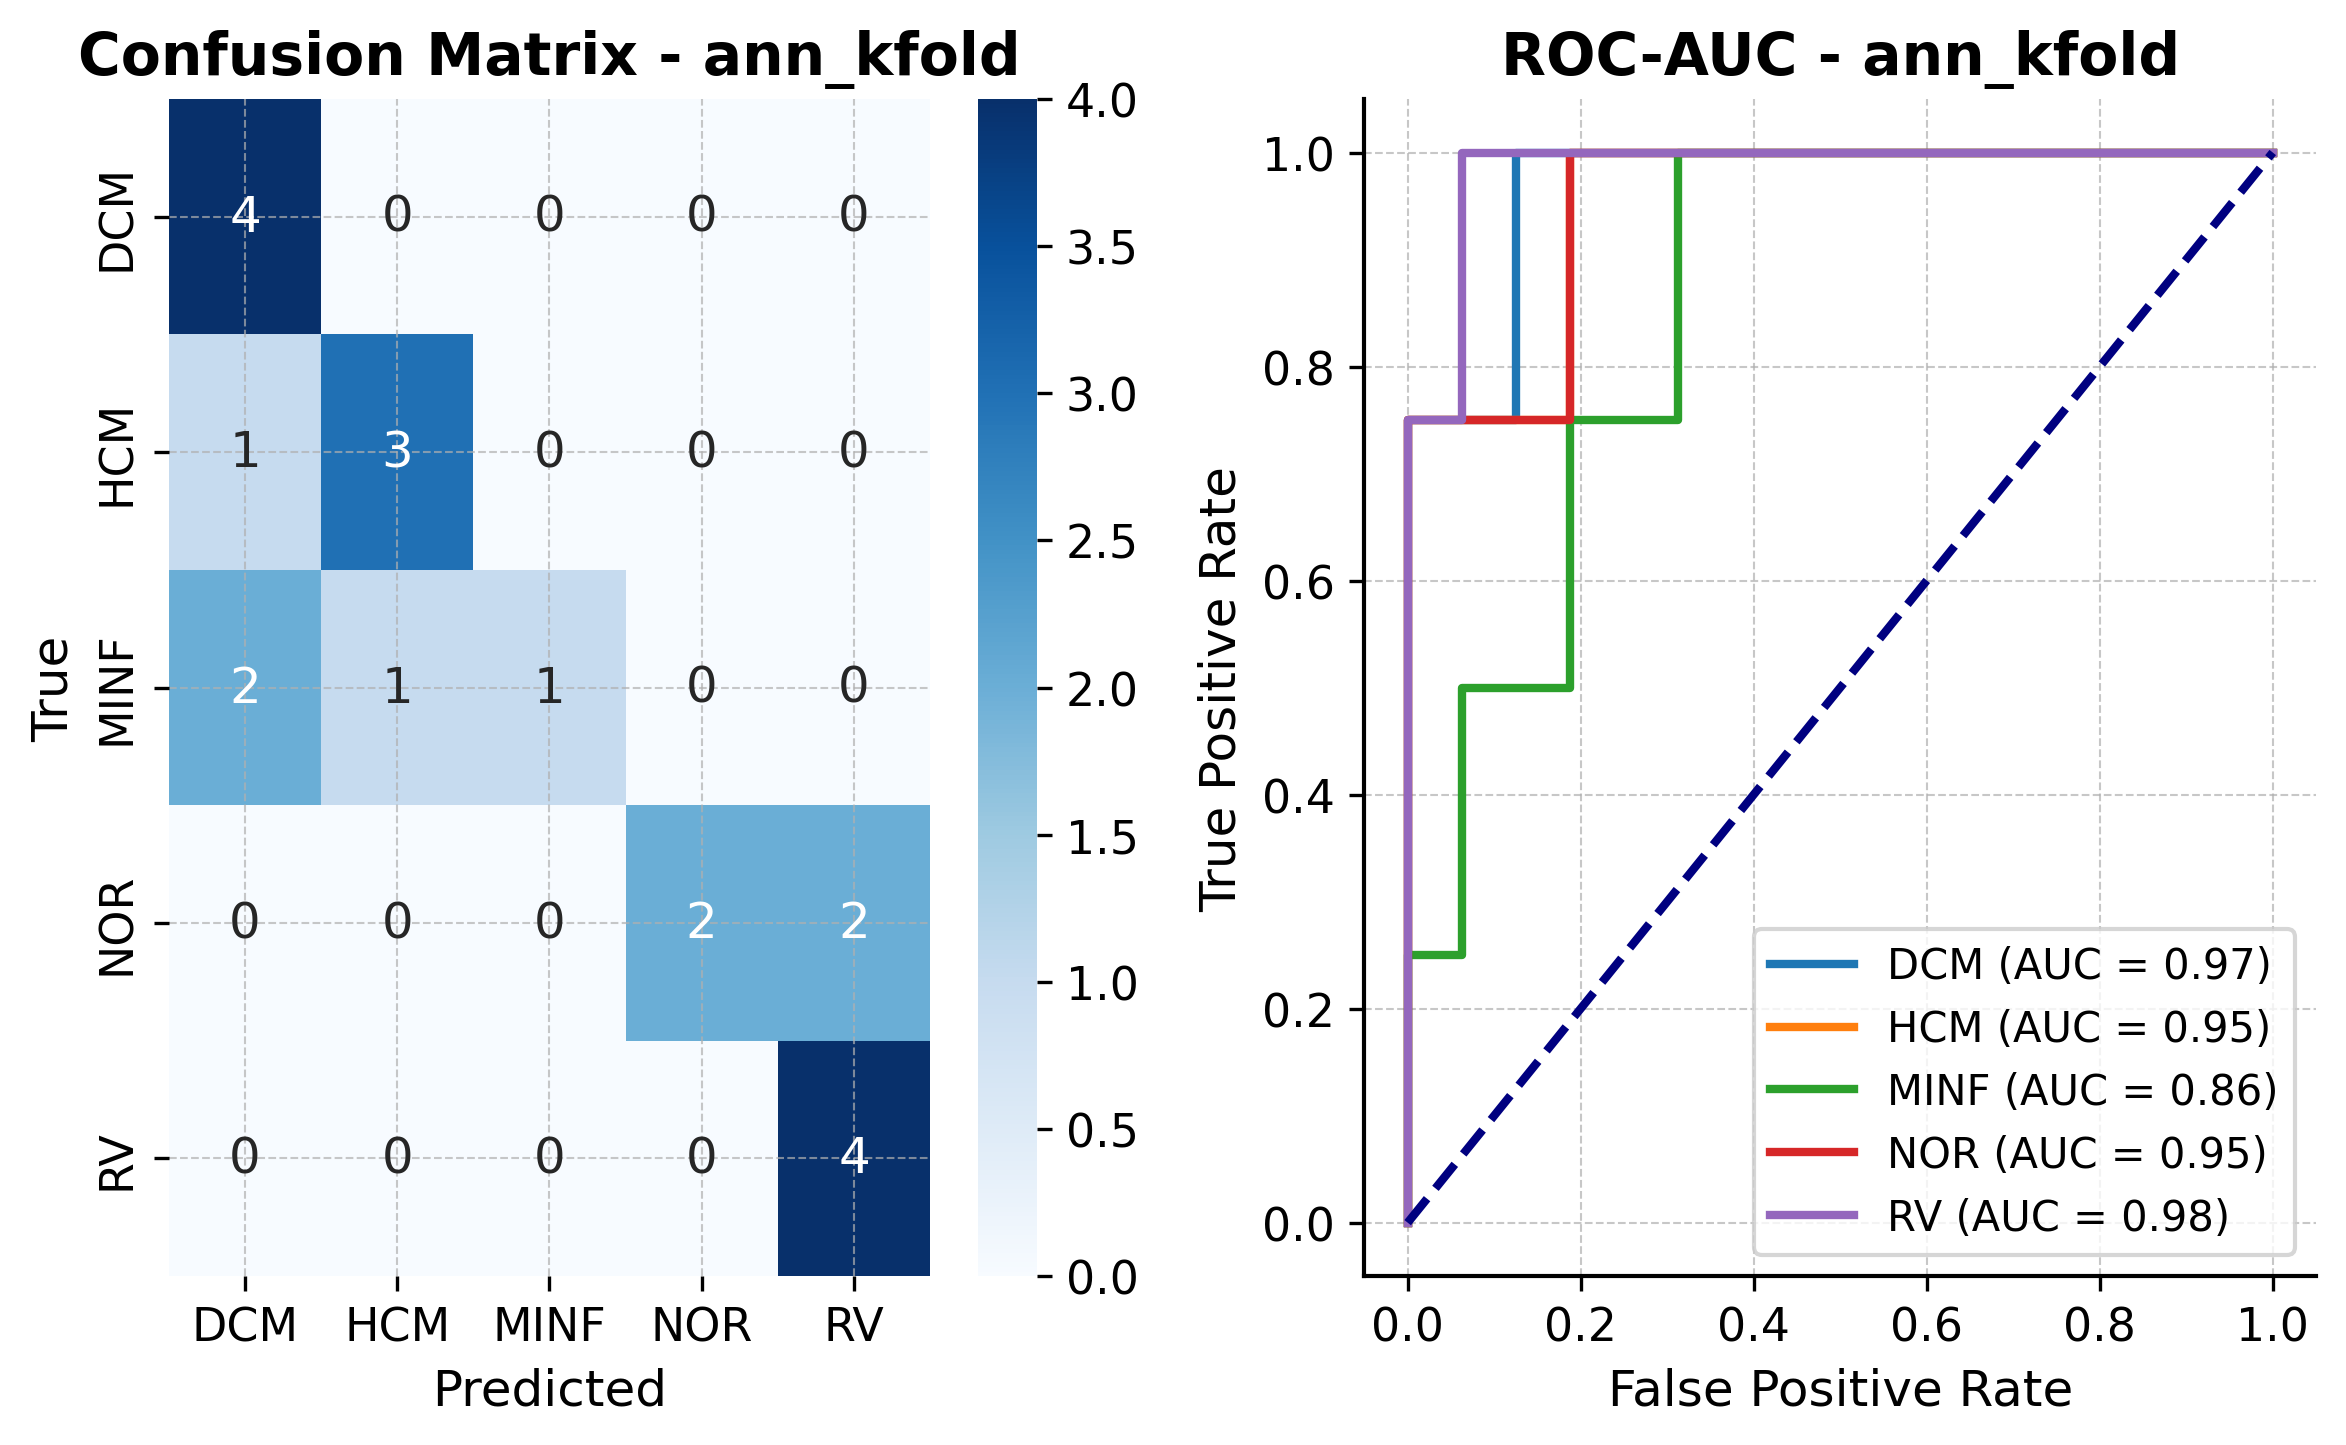
\includegraphics[width=0.99\textwidth]{../images/metrics/ann/ann_kfold_metrics.png}
	\end{center}
	\caption{Confusion matrix and ROC curves for the Artificial Neural Network
		(ANN) model trained with Stratified K-Fold cross-validation. DCM $=$ Dilated
		Cardiomyopathy, HCM $=$ Hypertrophic Cardiomyopathy, MINF $=$ Myocardial
		Infarction, NOR $=$ Normal, RV $=$ Right Ventricular abnormality.}
\end{figure}

\begin{figure}
	\begin{center}
		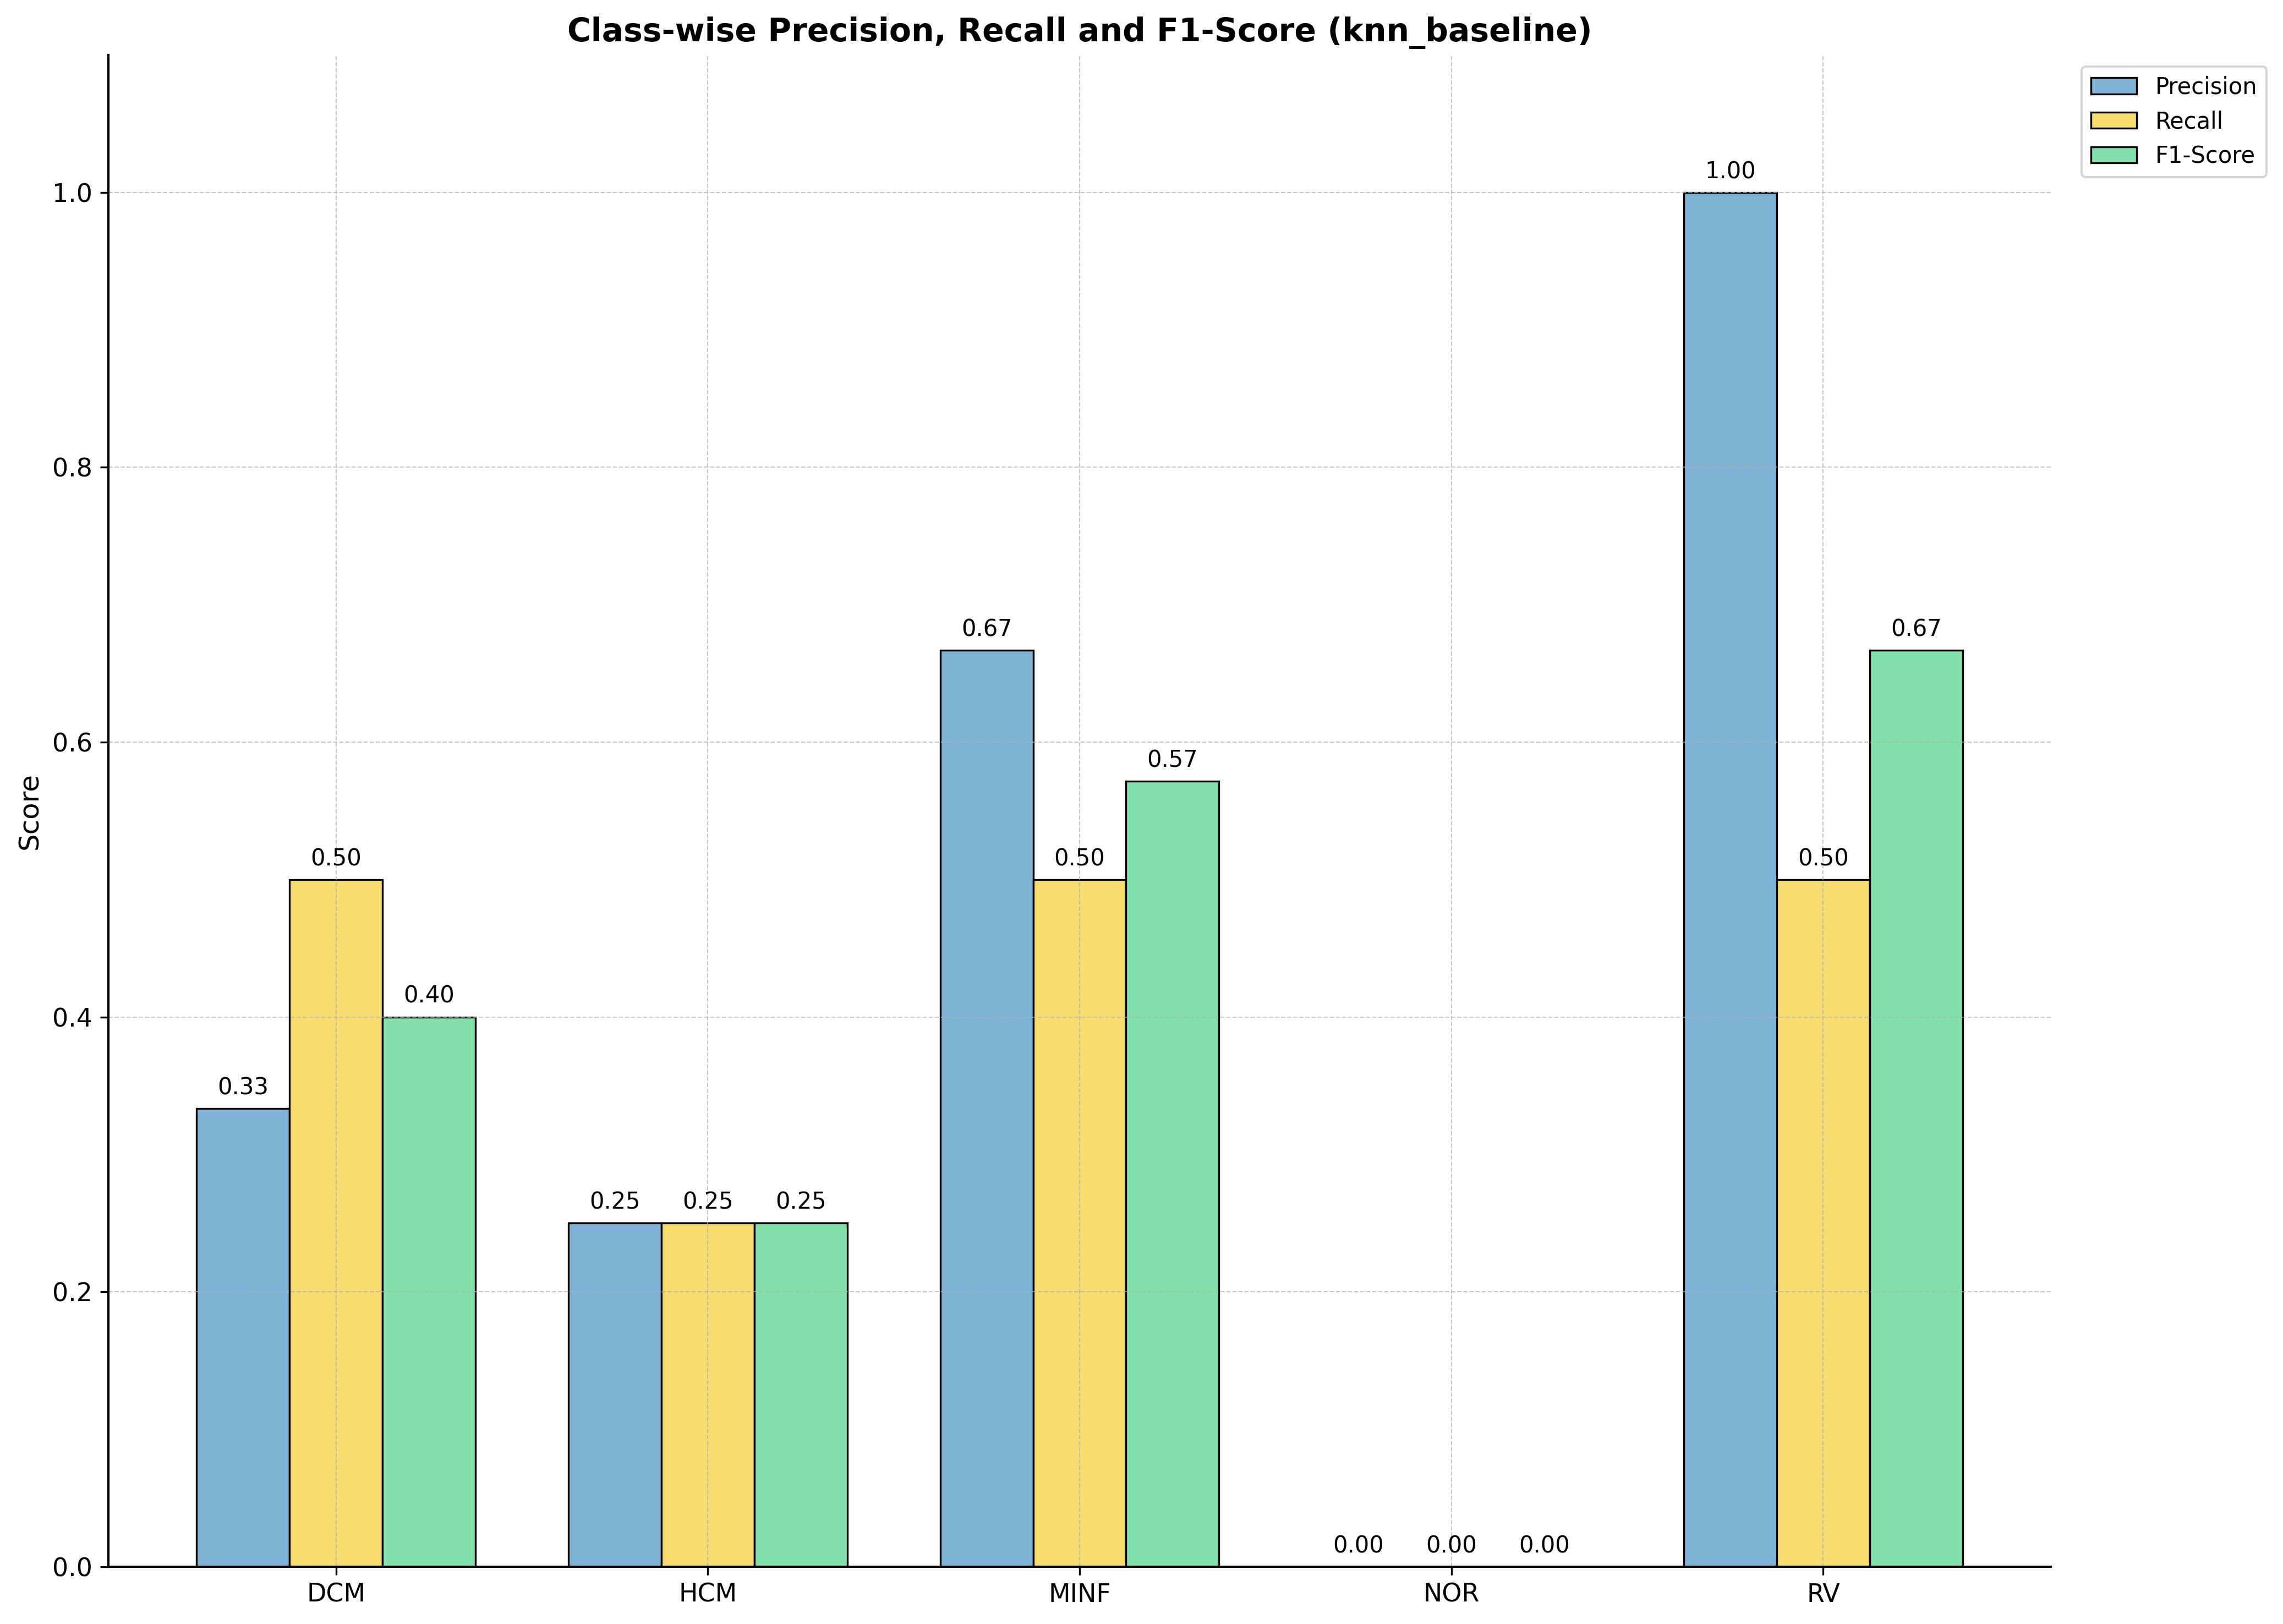
\includegraphics[width=0.85\textwidth]{../images/metrics/knn/knn_baseline_class_wise_metrics.png}
	\end{center}
	\caption{Class-wise Precision, Recall, and F1-Score for the k-Nearest
		Neighbors (KNN) model trained using no strategy. DCM $=$ Dilated
		Cardiomyopathy, HCM $=$ Hypertrophic Cardiomyopathy, MINF $=$ Myocardial
		Infarction, NOR $=$ Normal, RV $=$ Right Ventricular abnormality.}
\end{figure}

\begin{figure}
	\begin{center}
		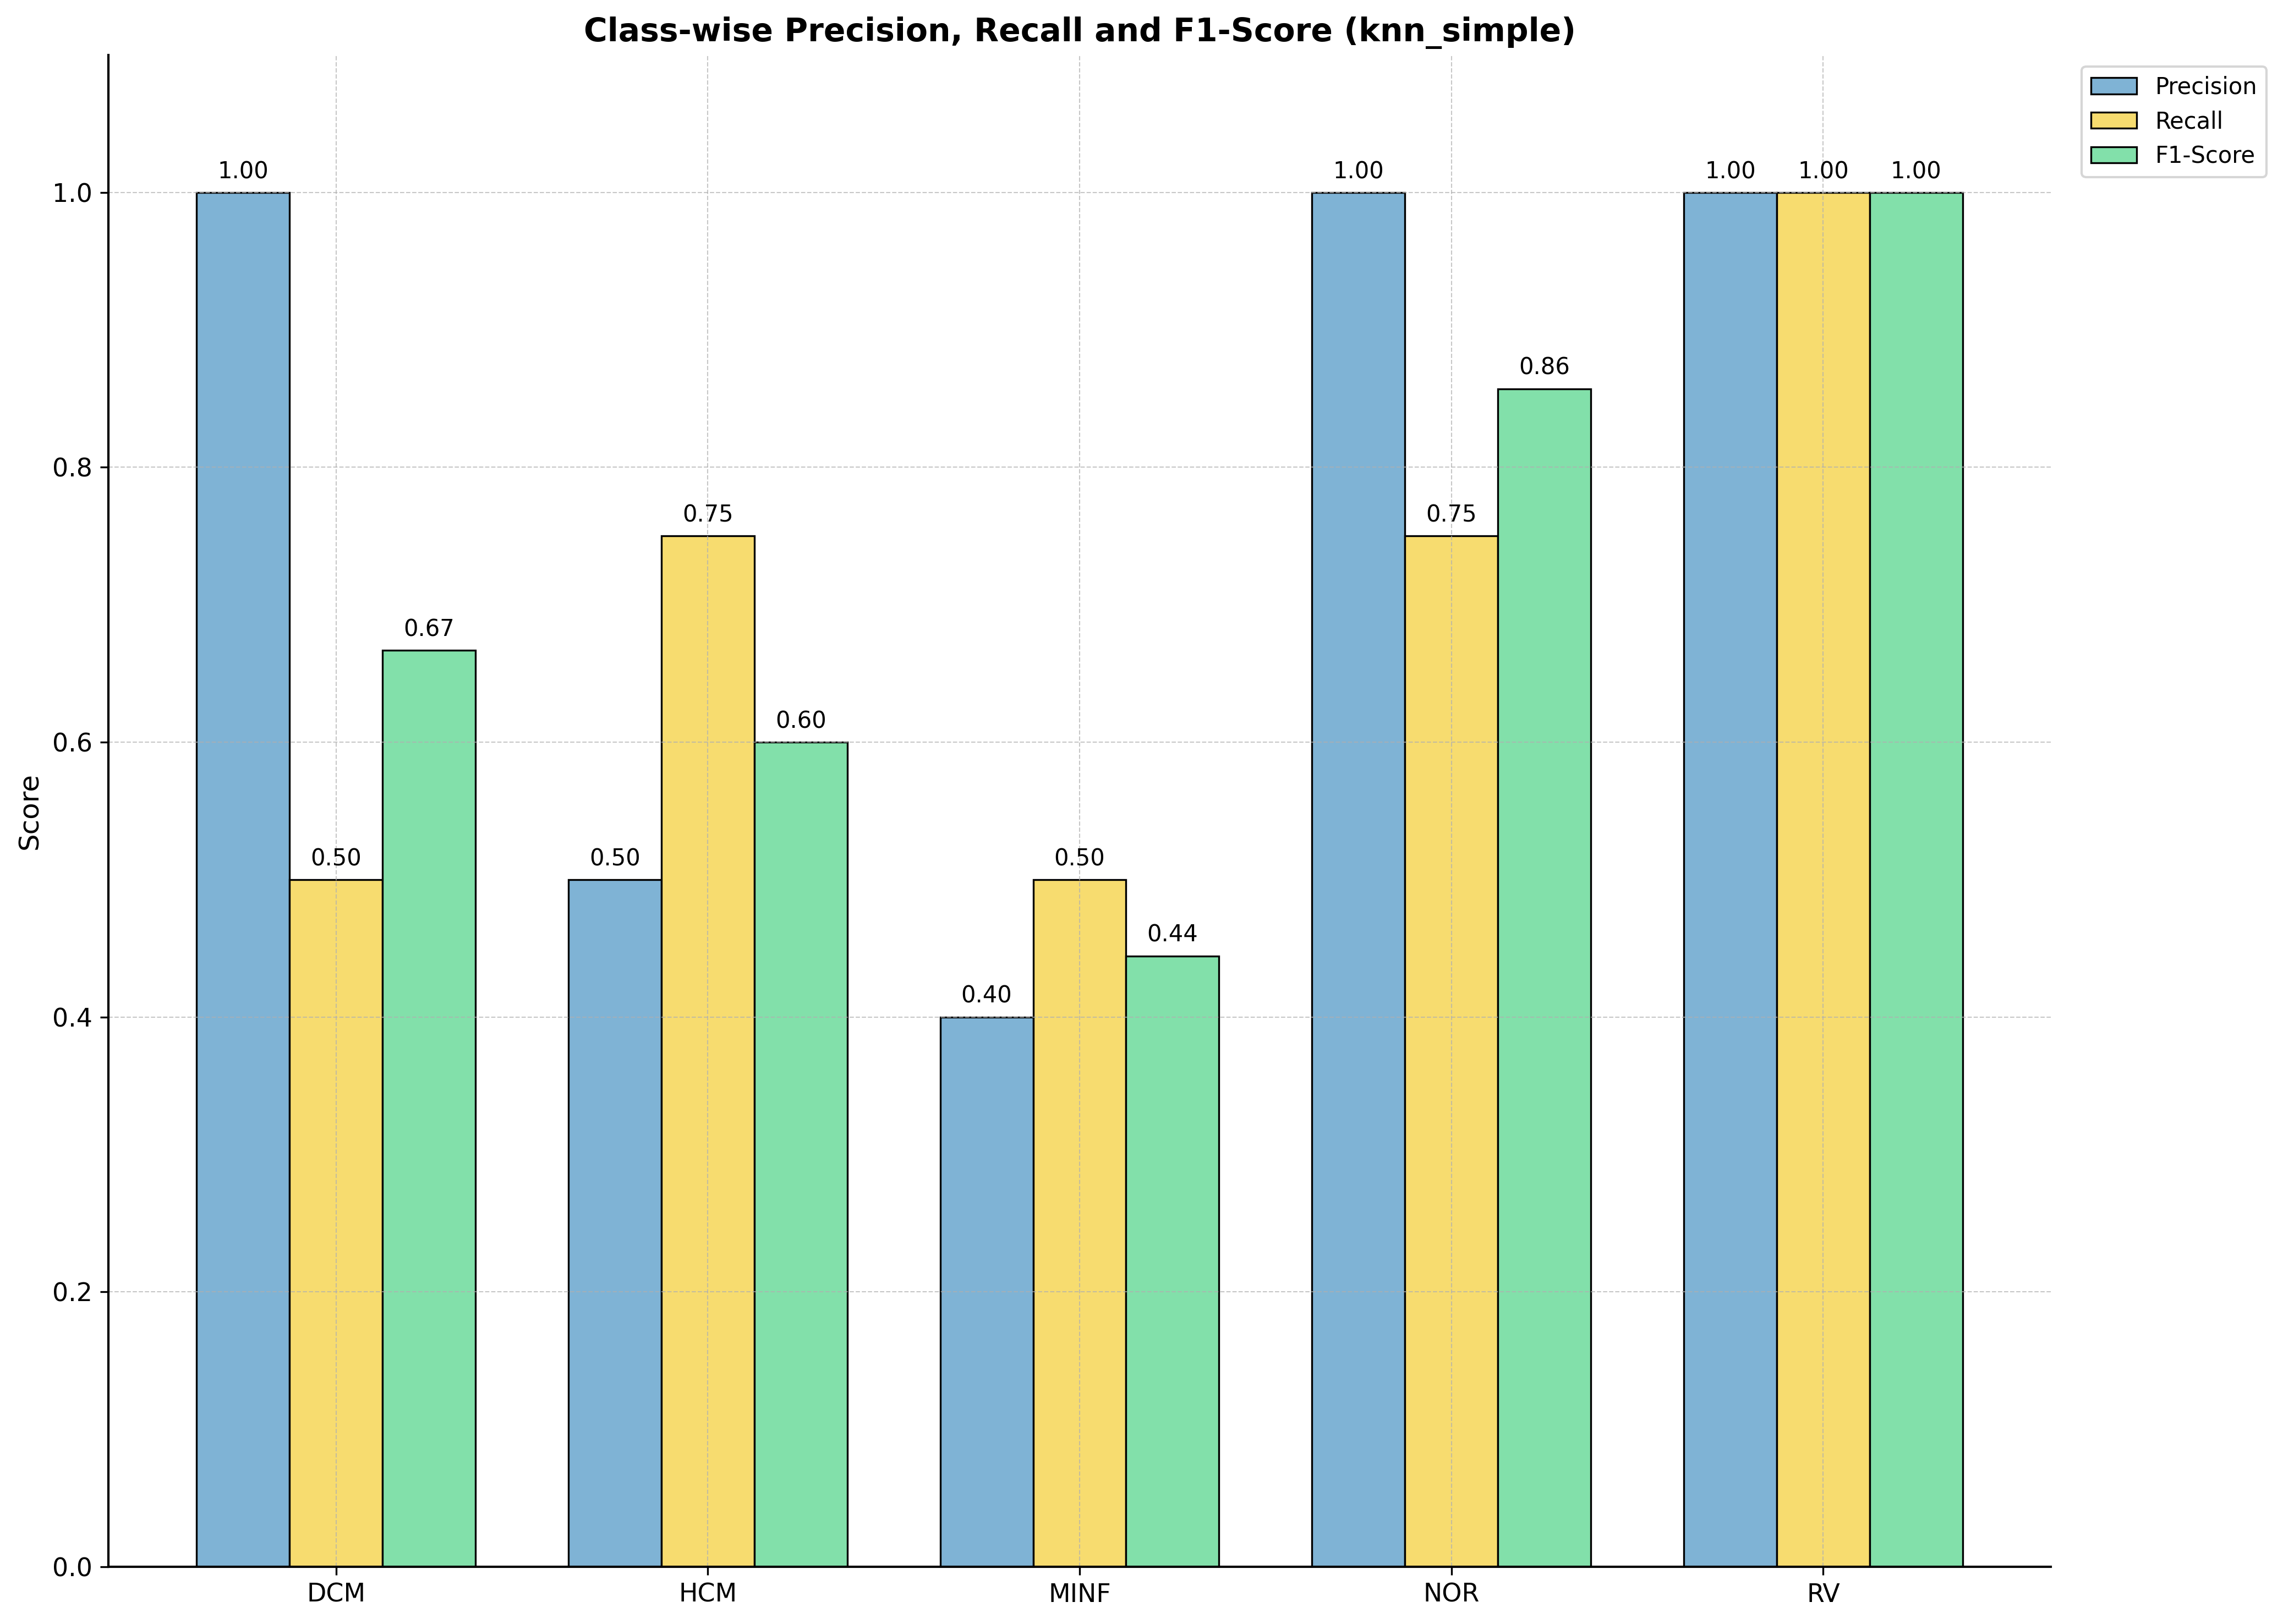
\includegraphics[width=0.85\textwidth]{../images/metrics/knn/knn_simple_class_wise_metrics.png}
	\end{center}
	\caption{Class-wise Precision, Recall, and F1-Score for the k-Nearest
		Neighbors (KNN) model trained using the Simple Split strategy. DCM $=$
		Dilated Cardiomyopathy, HCM $=$ Hypertrophic Cardiomyopathy, MINF $=$
		Myocardial Infarction, NOR $=$ Normal, RV $=$ Right Ventricular abnormality.}
\end{figure}

\begin{figure}
	\begin{center}
		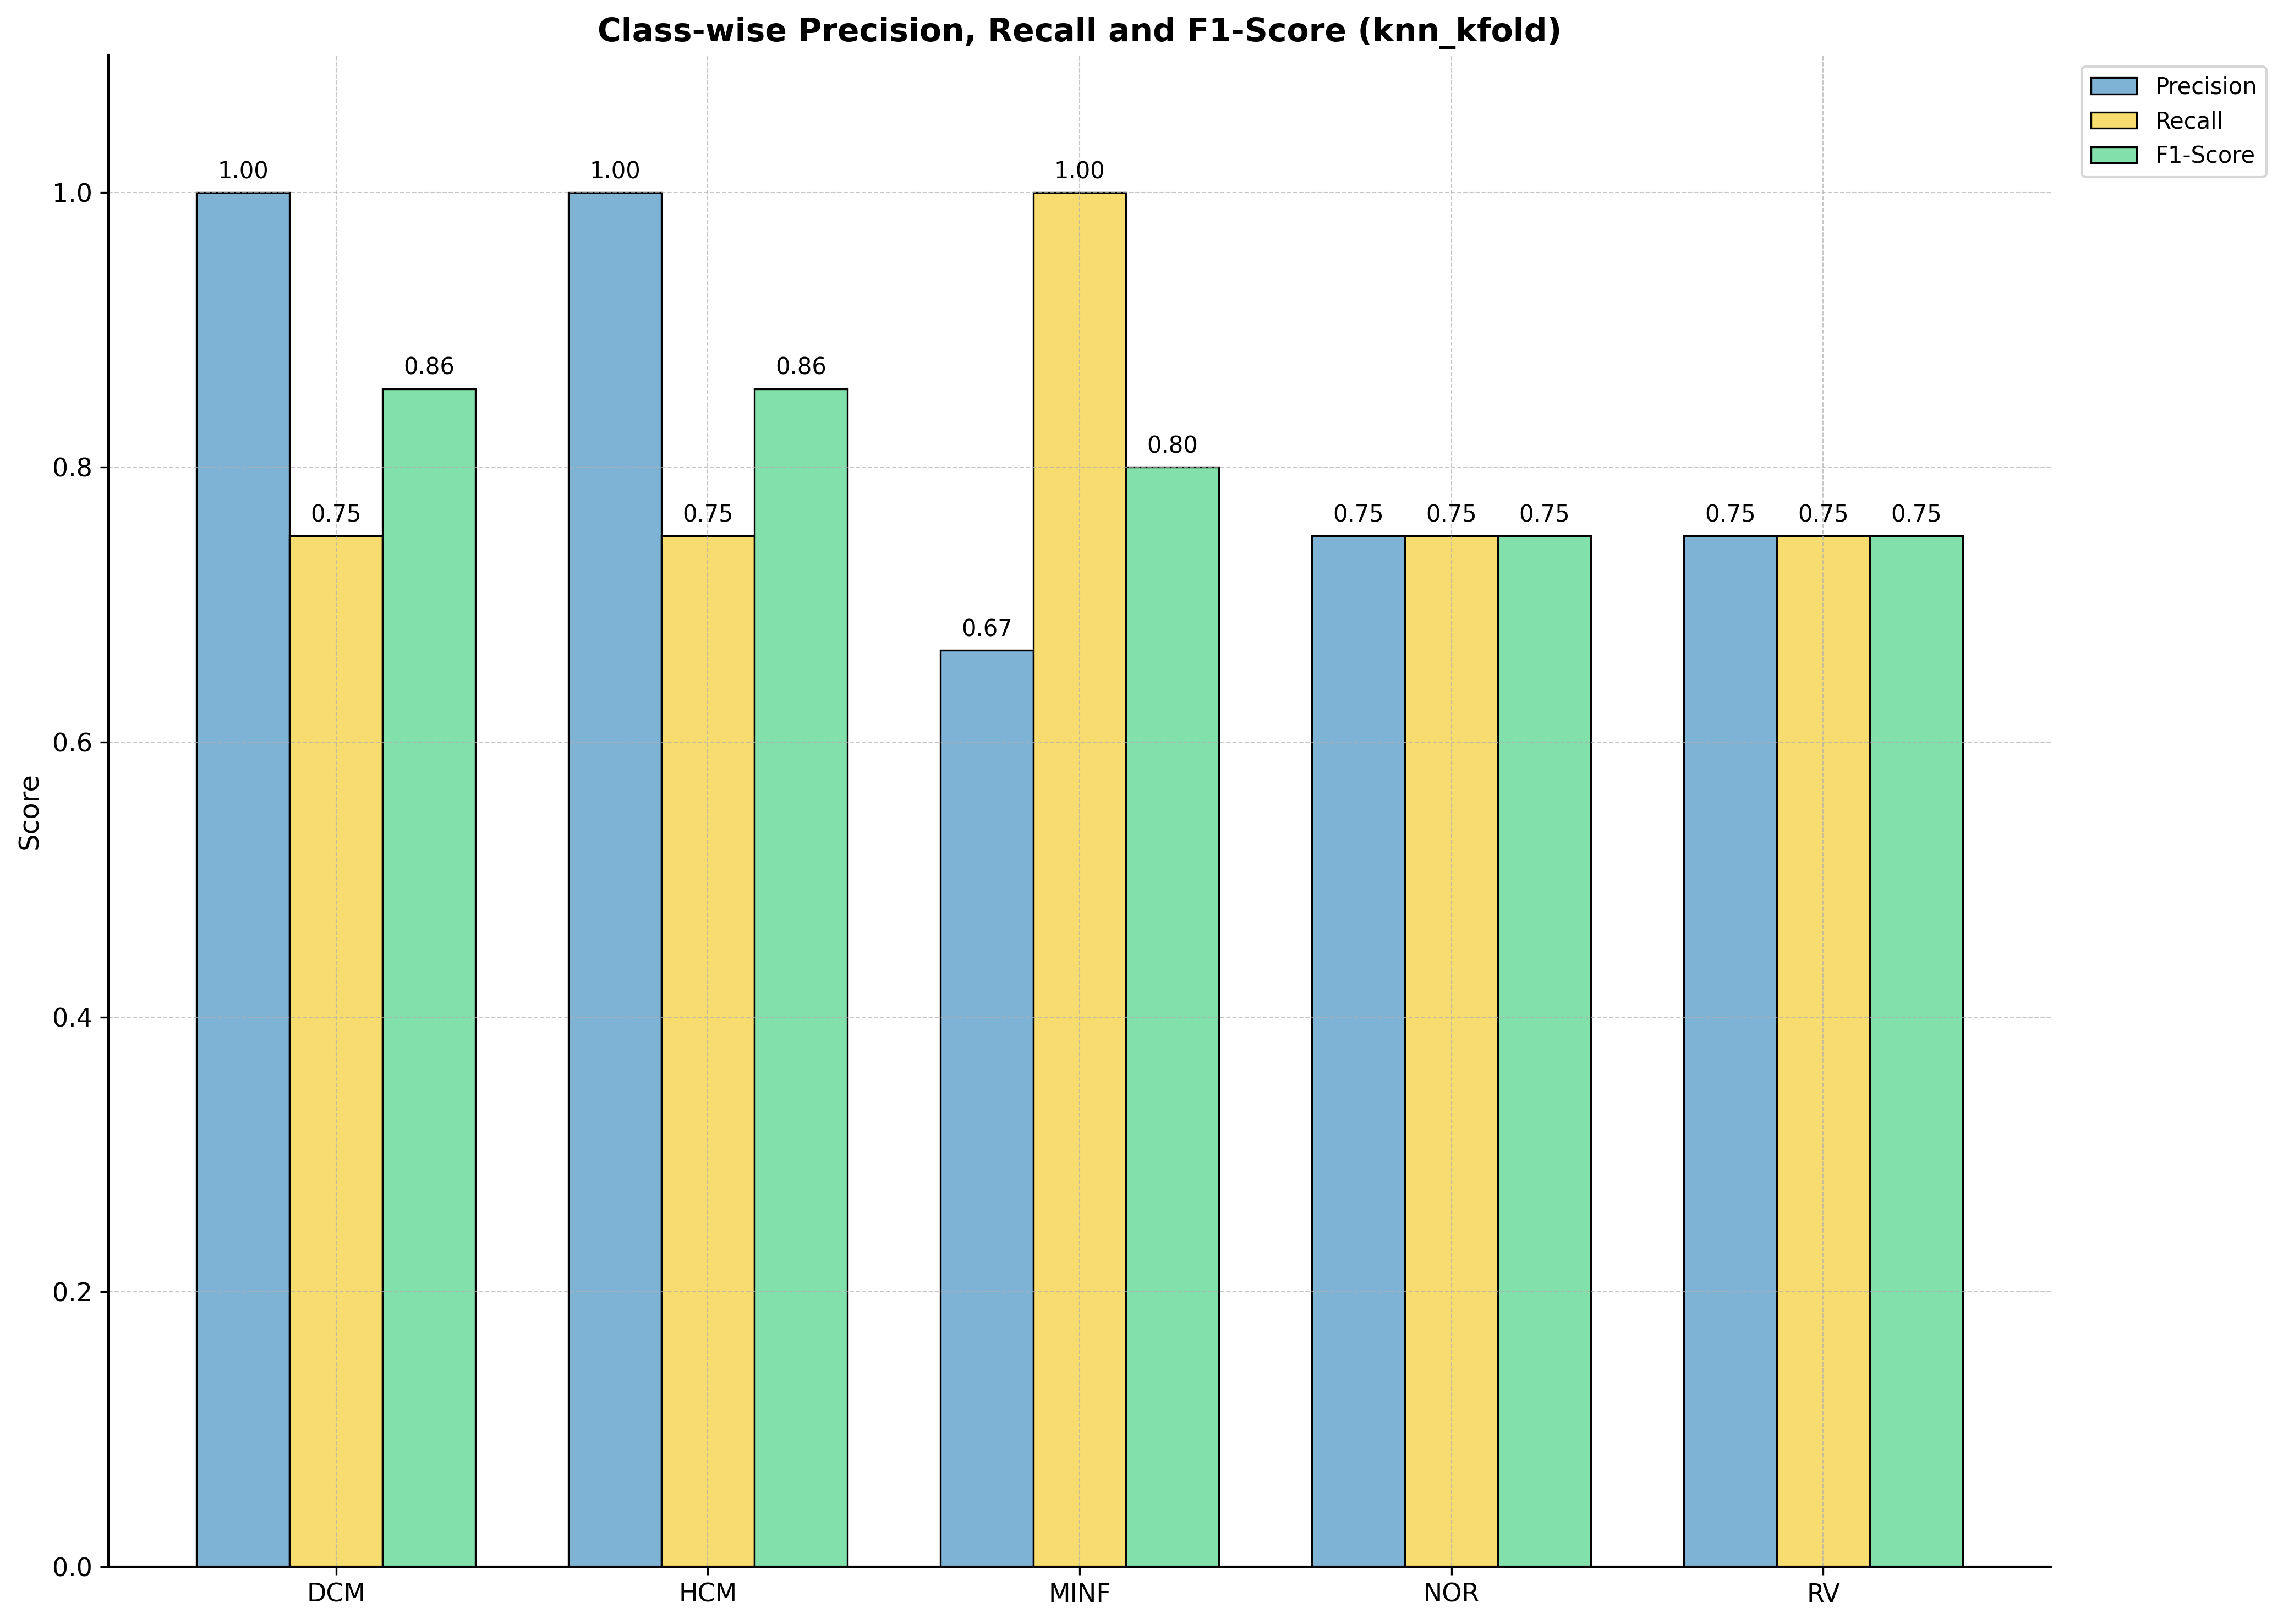
\includegraphics[width=0.85\textwidth]{../images/metrics/knn/knn_kfold_class_wise_metrics.png}
	\end{center}
	\caption{Class-wise Precision, Recall, and F1-Score for the k-Nearest
		Neighbors (KNN) model trained with Stratified K-Fold cross-validation. DCM
		$=$ Dilated Cardiomyopathy, HCM $=$ Hypertrophic Cardiomyopathy, MINF $=$
		Myocardial Infarction, NOR $=$ Normal, RV $=$ Right Ventricular abnormality.}
\end{figure}

\begin{figure}
	\begin{center}
		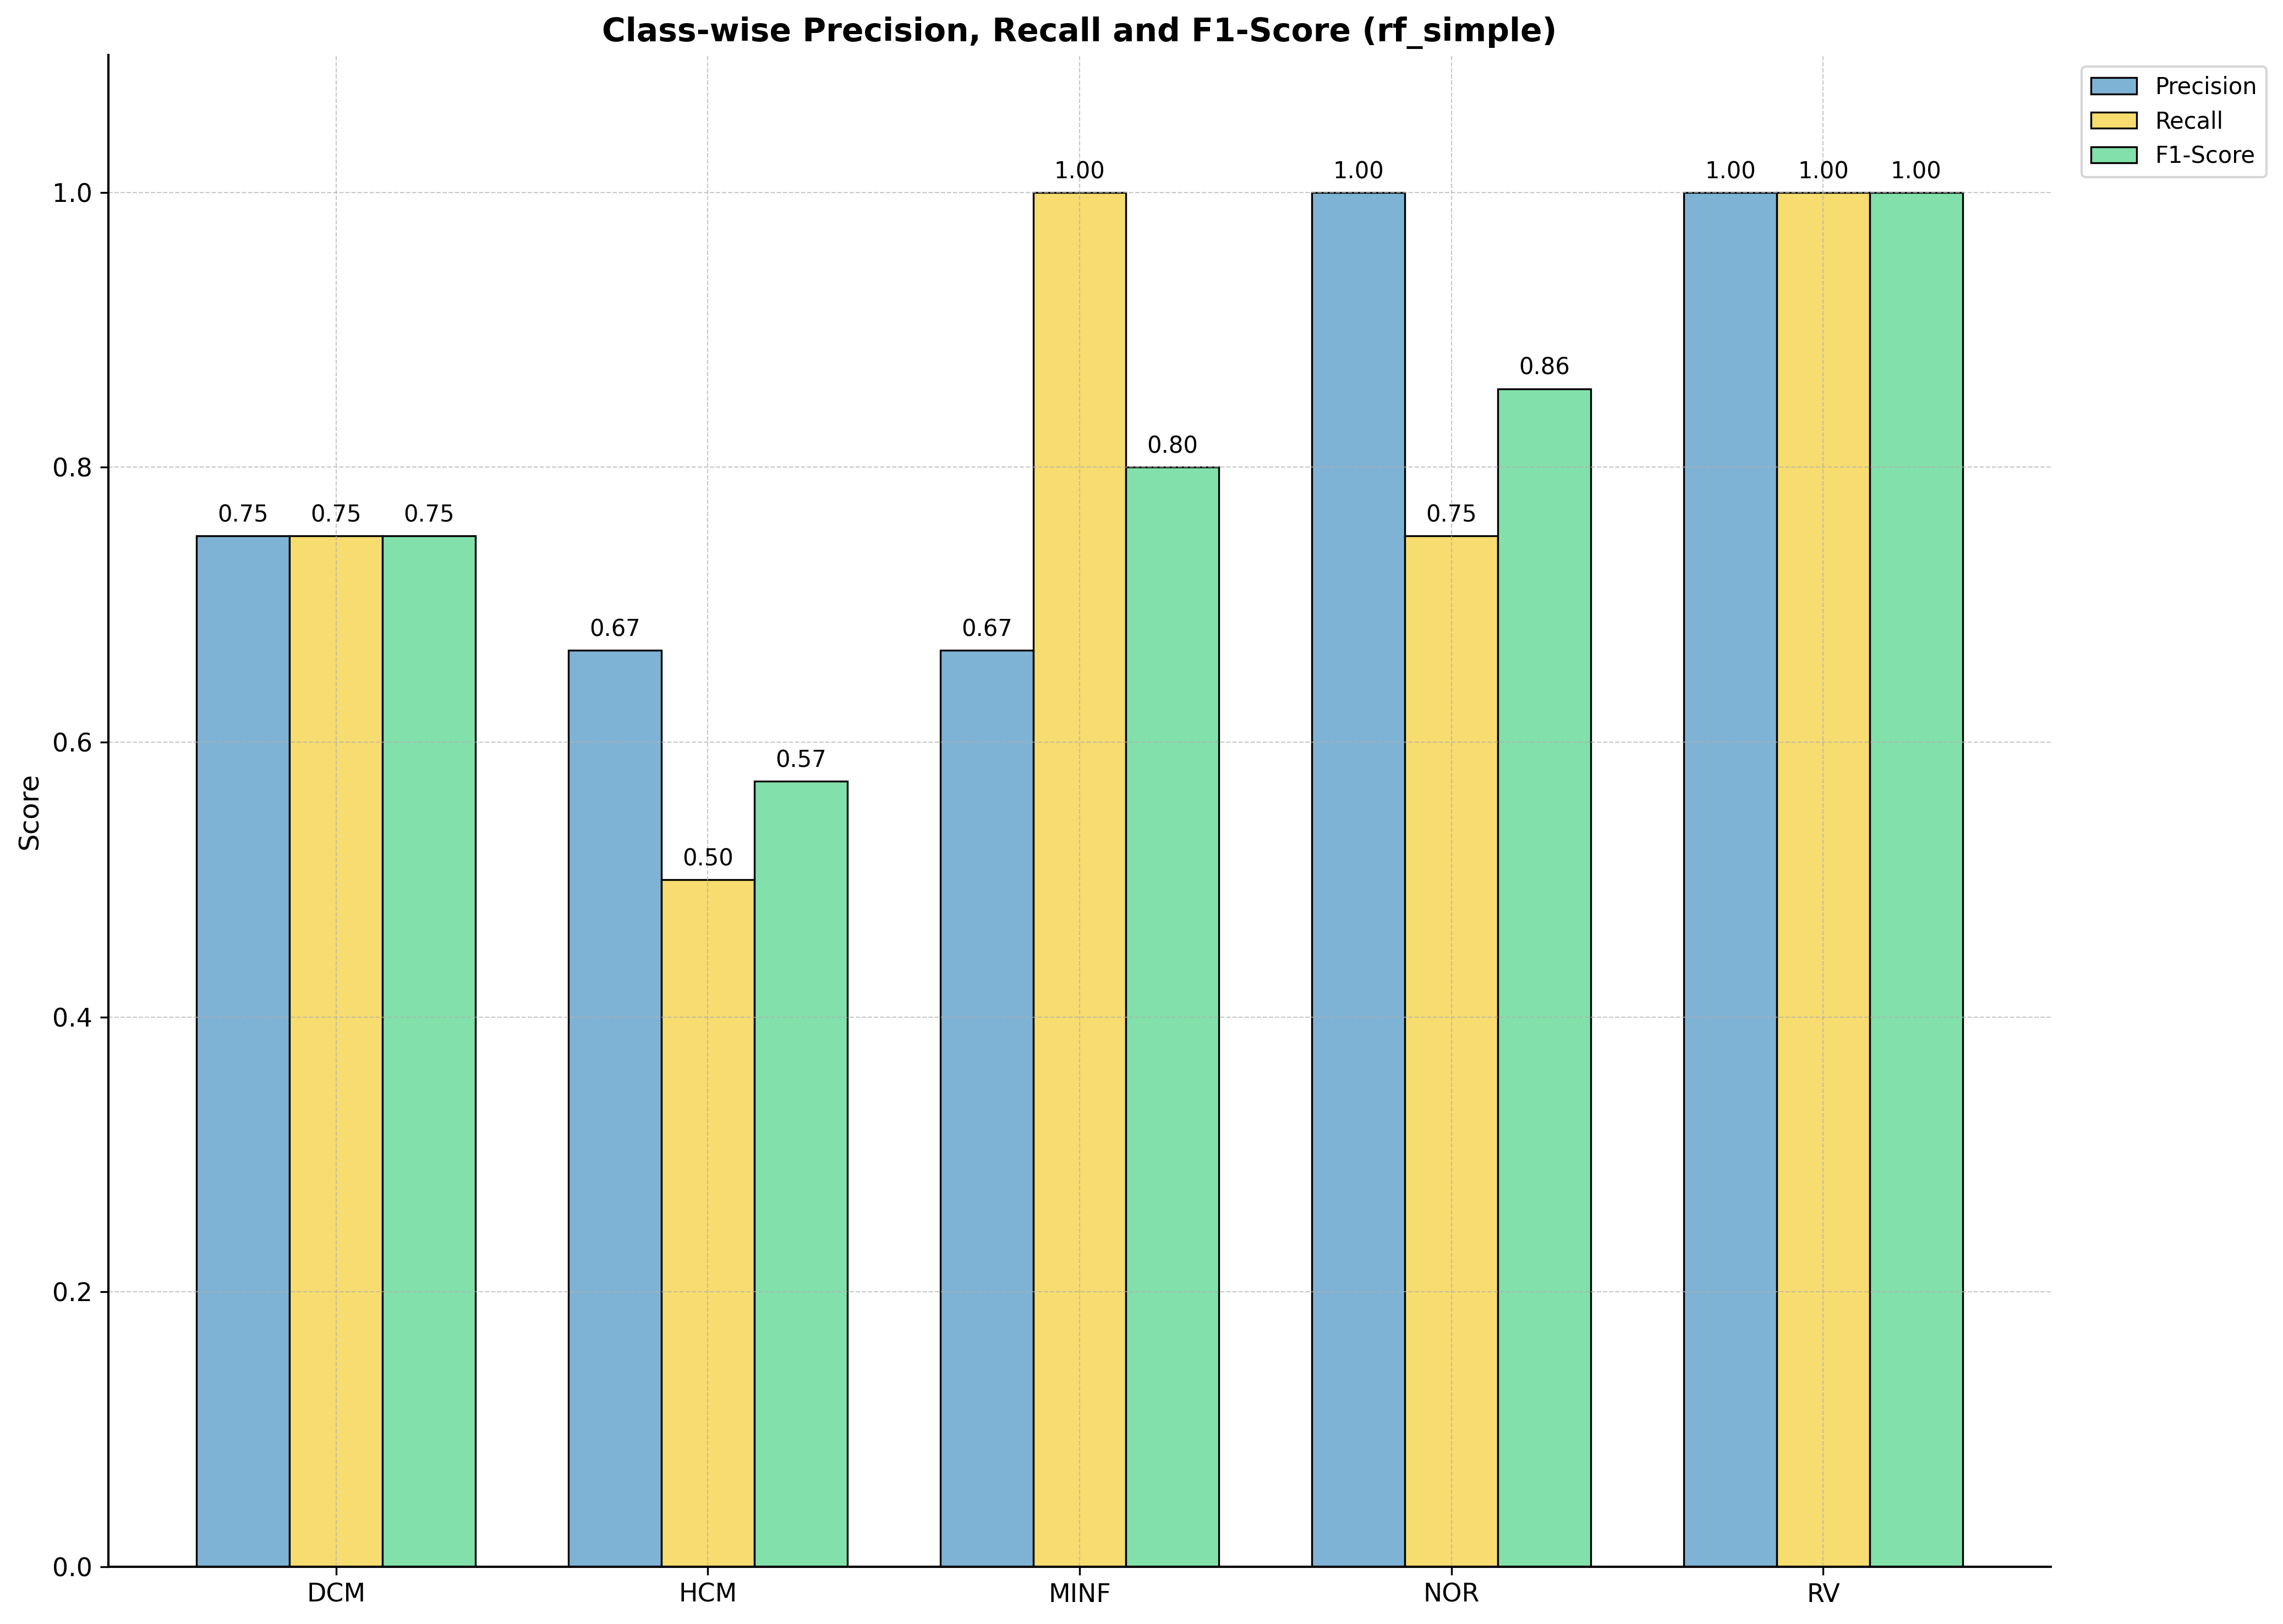
\includegraphics[width=0.85\textwidth]{../images/metrics/rf/rf_simple_class_wise_metrics.png}
	\end{center}
	\caption{Class-wise Precision, Recall, and F1-Score for the Random Forest
		(RF) model trained using the Simple Split strategy. DCM $=$ Dilated
		Cardiomyopathy, HCM $=$ Hypertrophic Cardiomyopathy, MINF $=$ Myocardial
		Infarction, NOR $=$ Normal, RV $=$ Right Ventricular abnormality.}
\end{figure}

\begin{figure}
	\begin{center}
		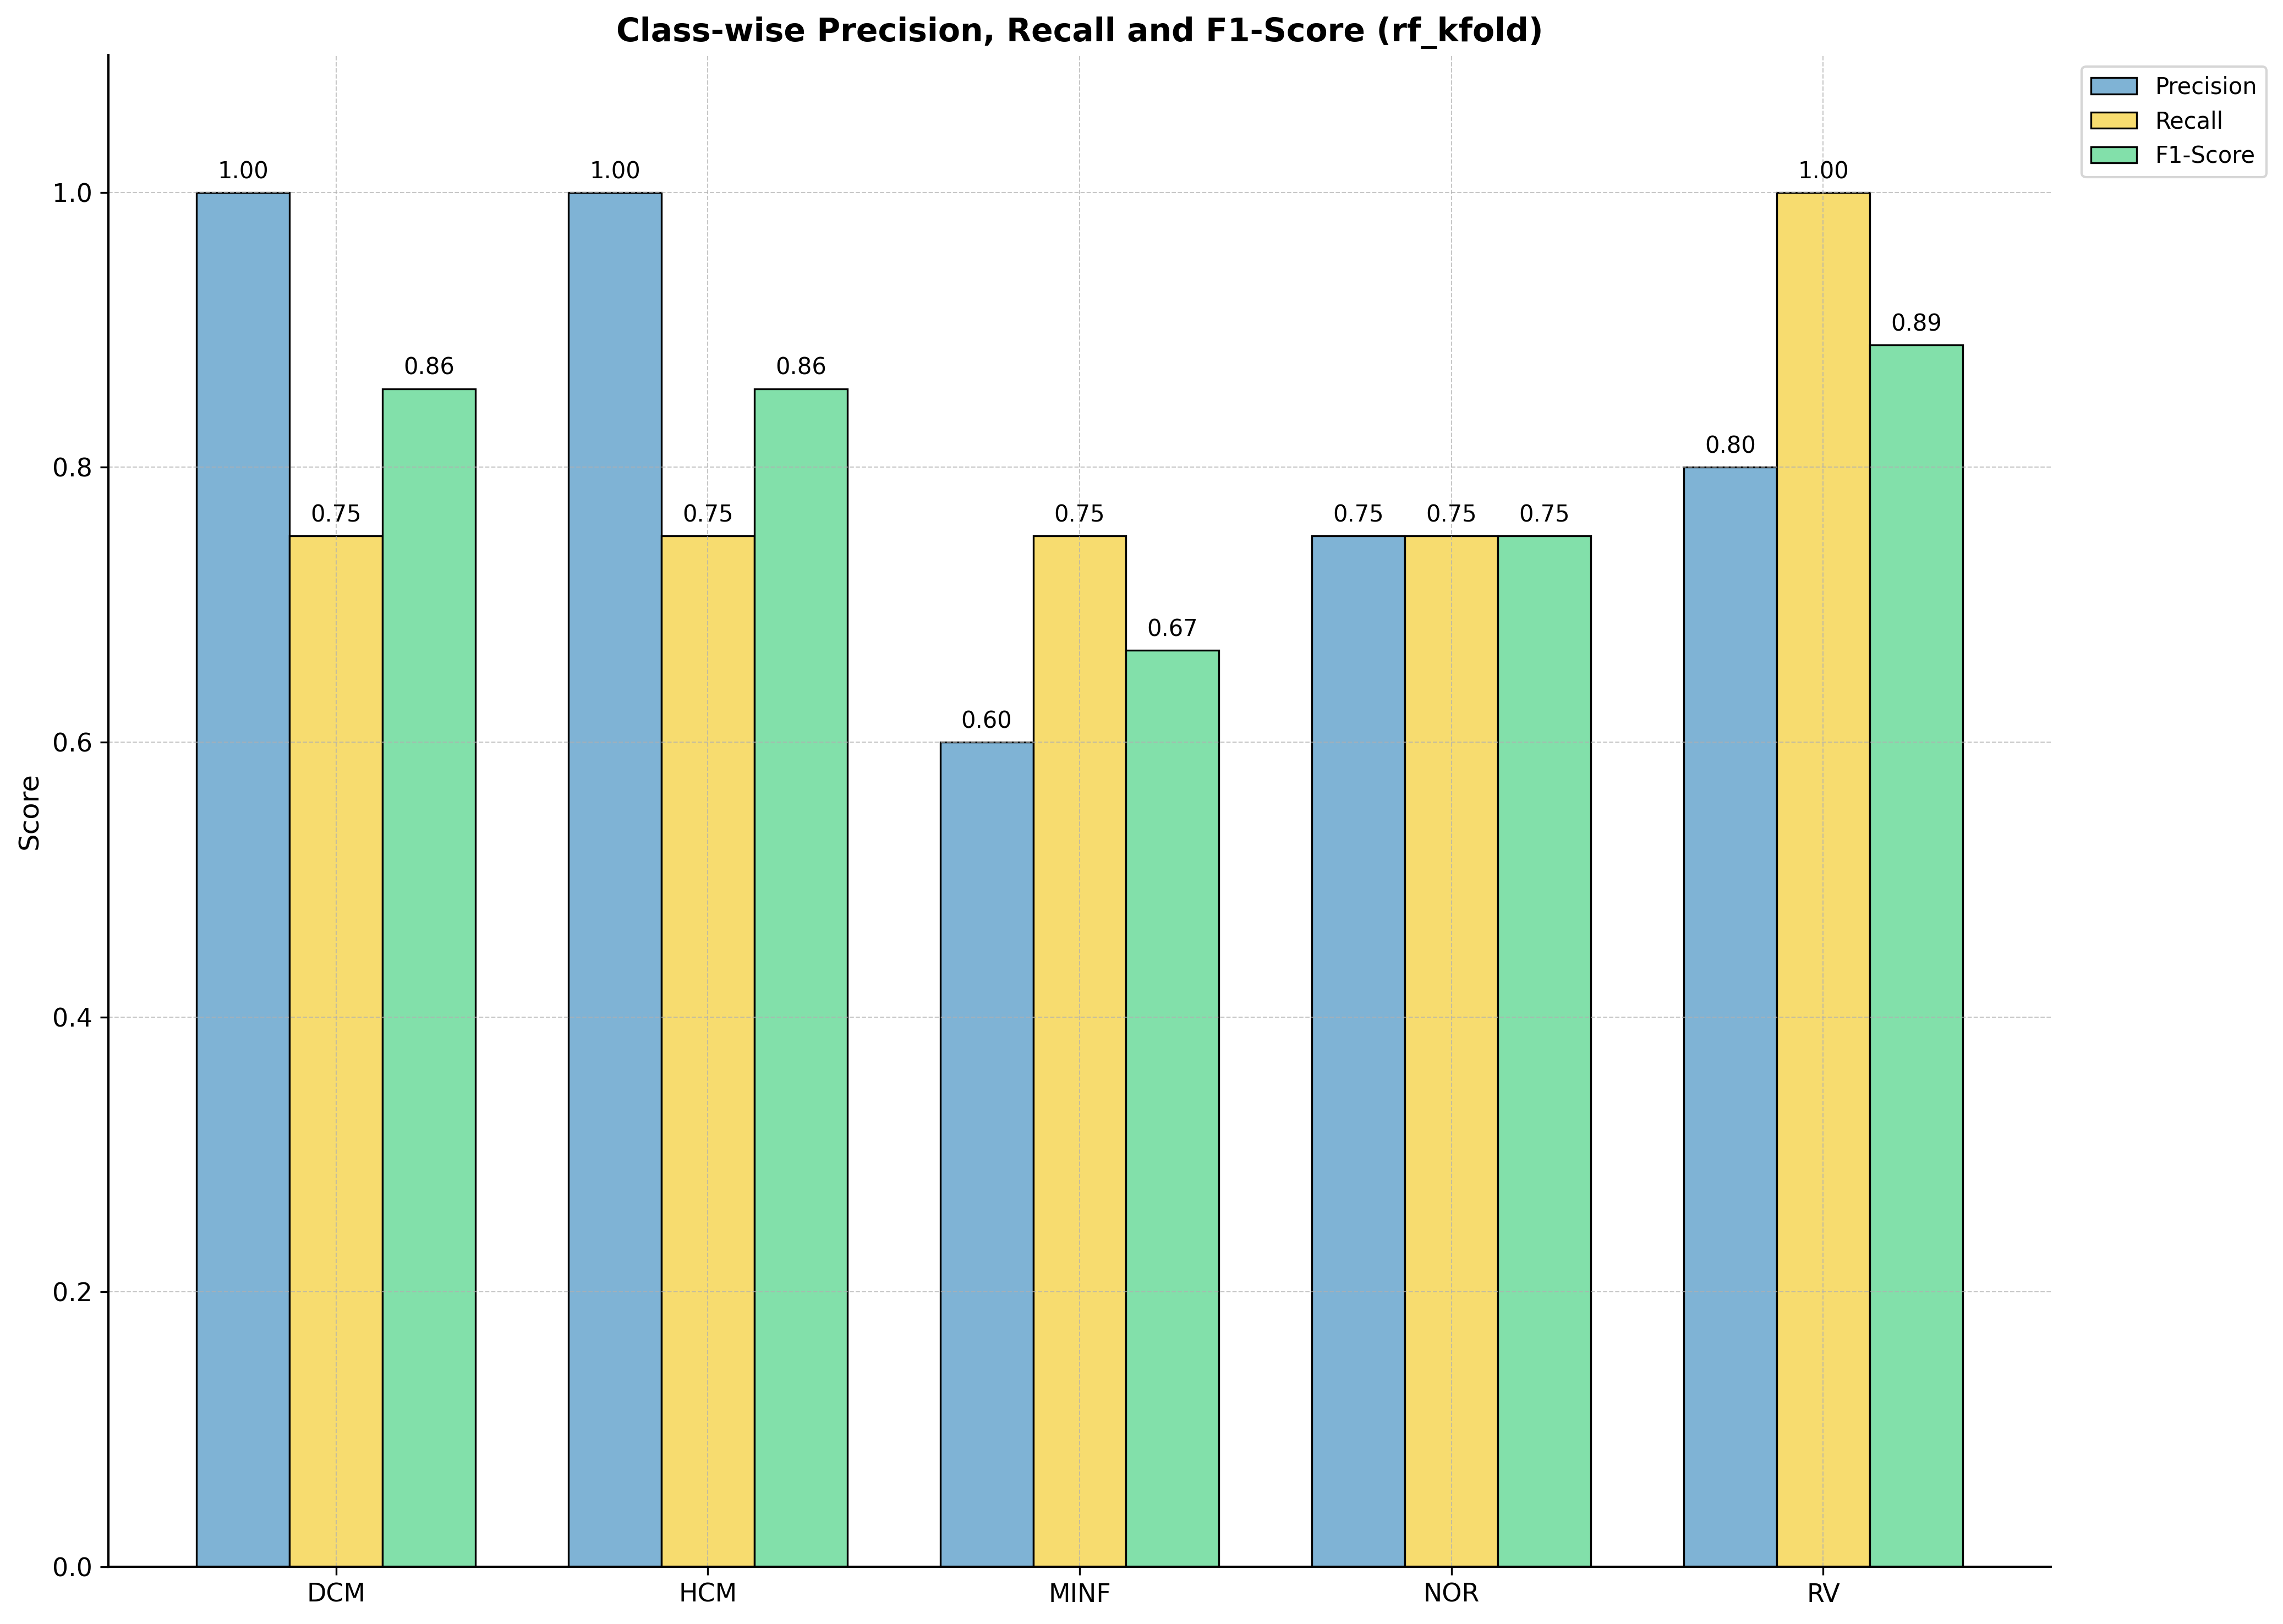
\includegraphics[width=0.85\textwidth]{../images/metrics/rf/rf_kfold_class_wise_metrics.png}
	\end{center}
	\caption{Class-wise Precision, Recall, and F1-Score for the Random Forest
		(RF) model trained with Stratified K-Fold cross-validation. DCM $=$ Dilated
		Cardiomyopathy, HCM $=$ Hypertrophic Cardiomyopathy, MINF $=$ Myocardial
		Infarction, NOR $=$ Normal, RV $=$ Right Ventricular abnormality.}
\end{figure}

\begin{figure}
	\begin{center}
		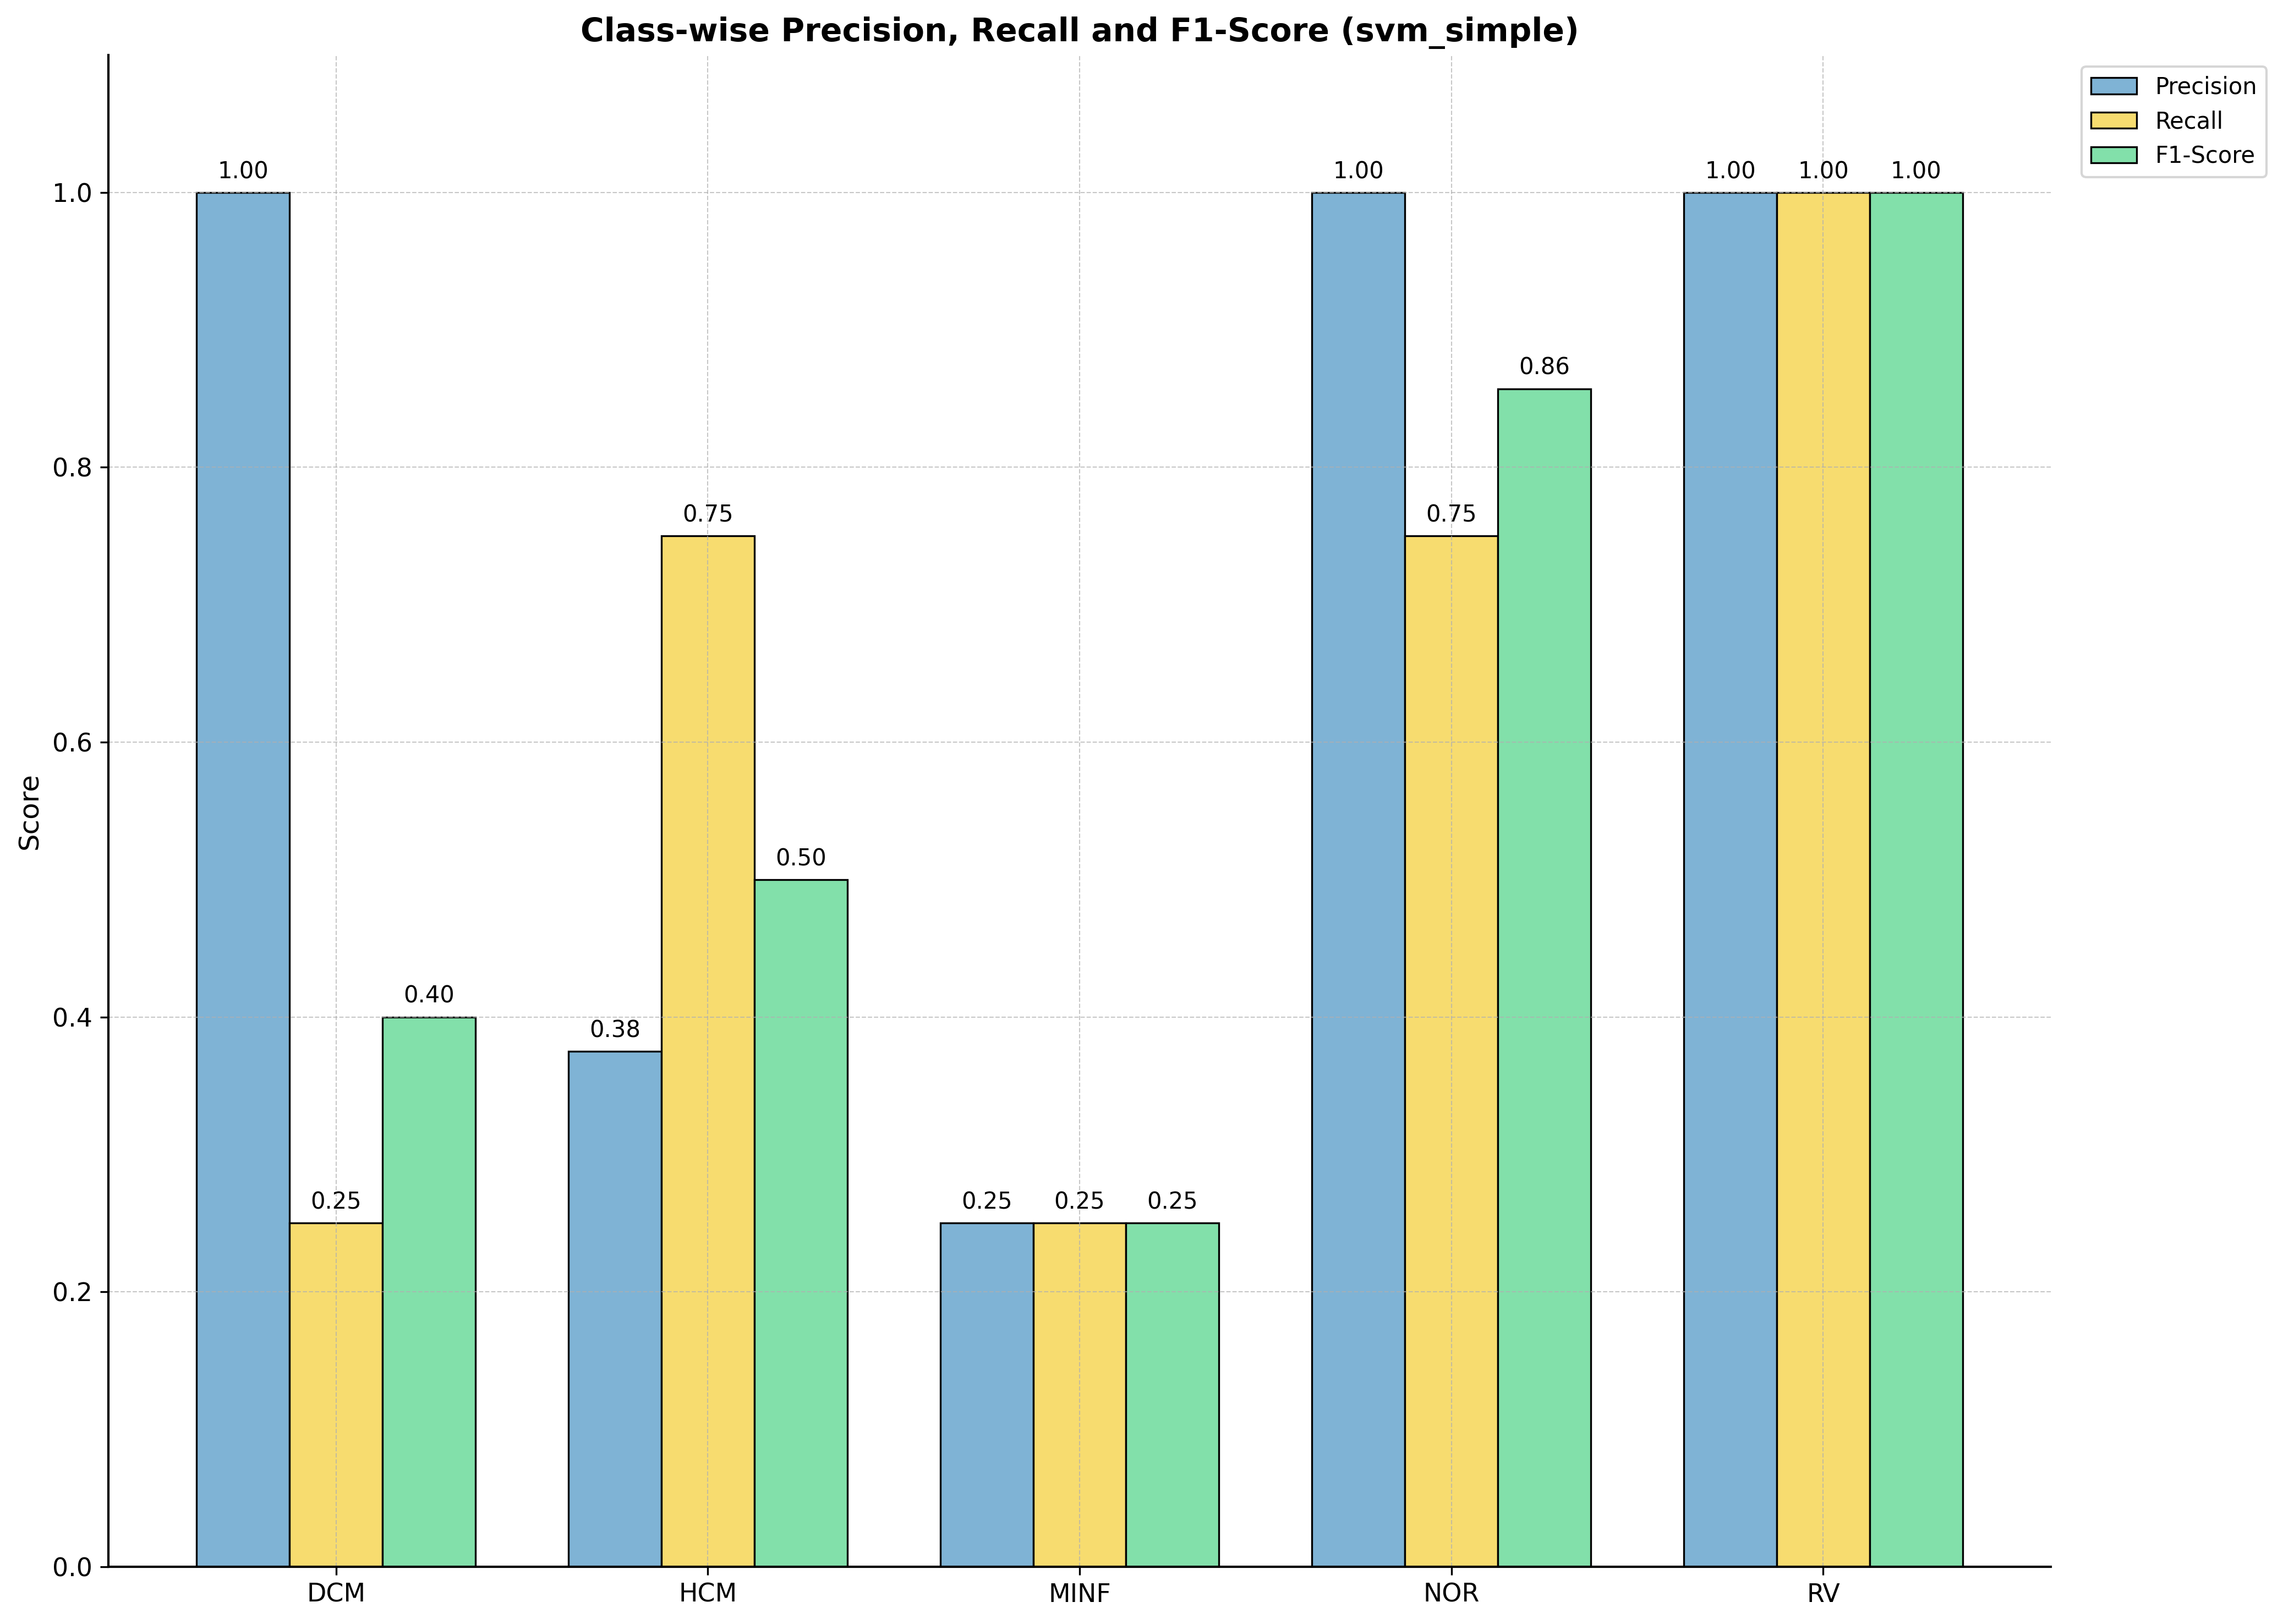
\includegraphics[width=0.85\textwidth]{../images/metrics/svm/svm_simple_class_wise_metrics.png}
	\end{center}
	\caption{Class-wise Precision, Recall, and F1-Score for the Support Vector
		Machine (SVM) model trained using the Simple Split strategy. DCM $=$ Dilated
		Cardiomyopathy, HCM $=$ Hypertrophic Cardiomyopathy, MINF $=$ Myocardial
		Infarction, NOR $=$ Normal, RV $=$ Right Ventricular abnormality.}
\end{figure}

\begin{figure}
	\begin{center}
		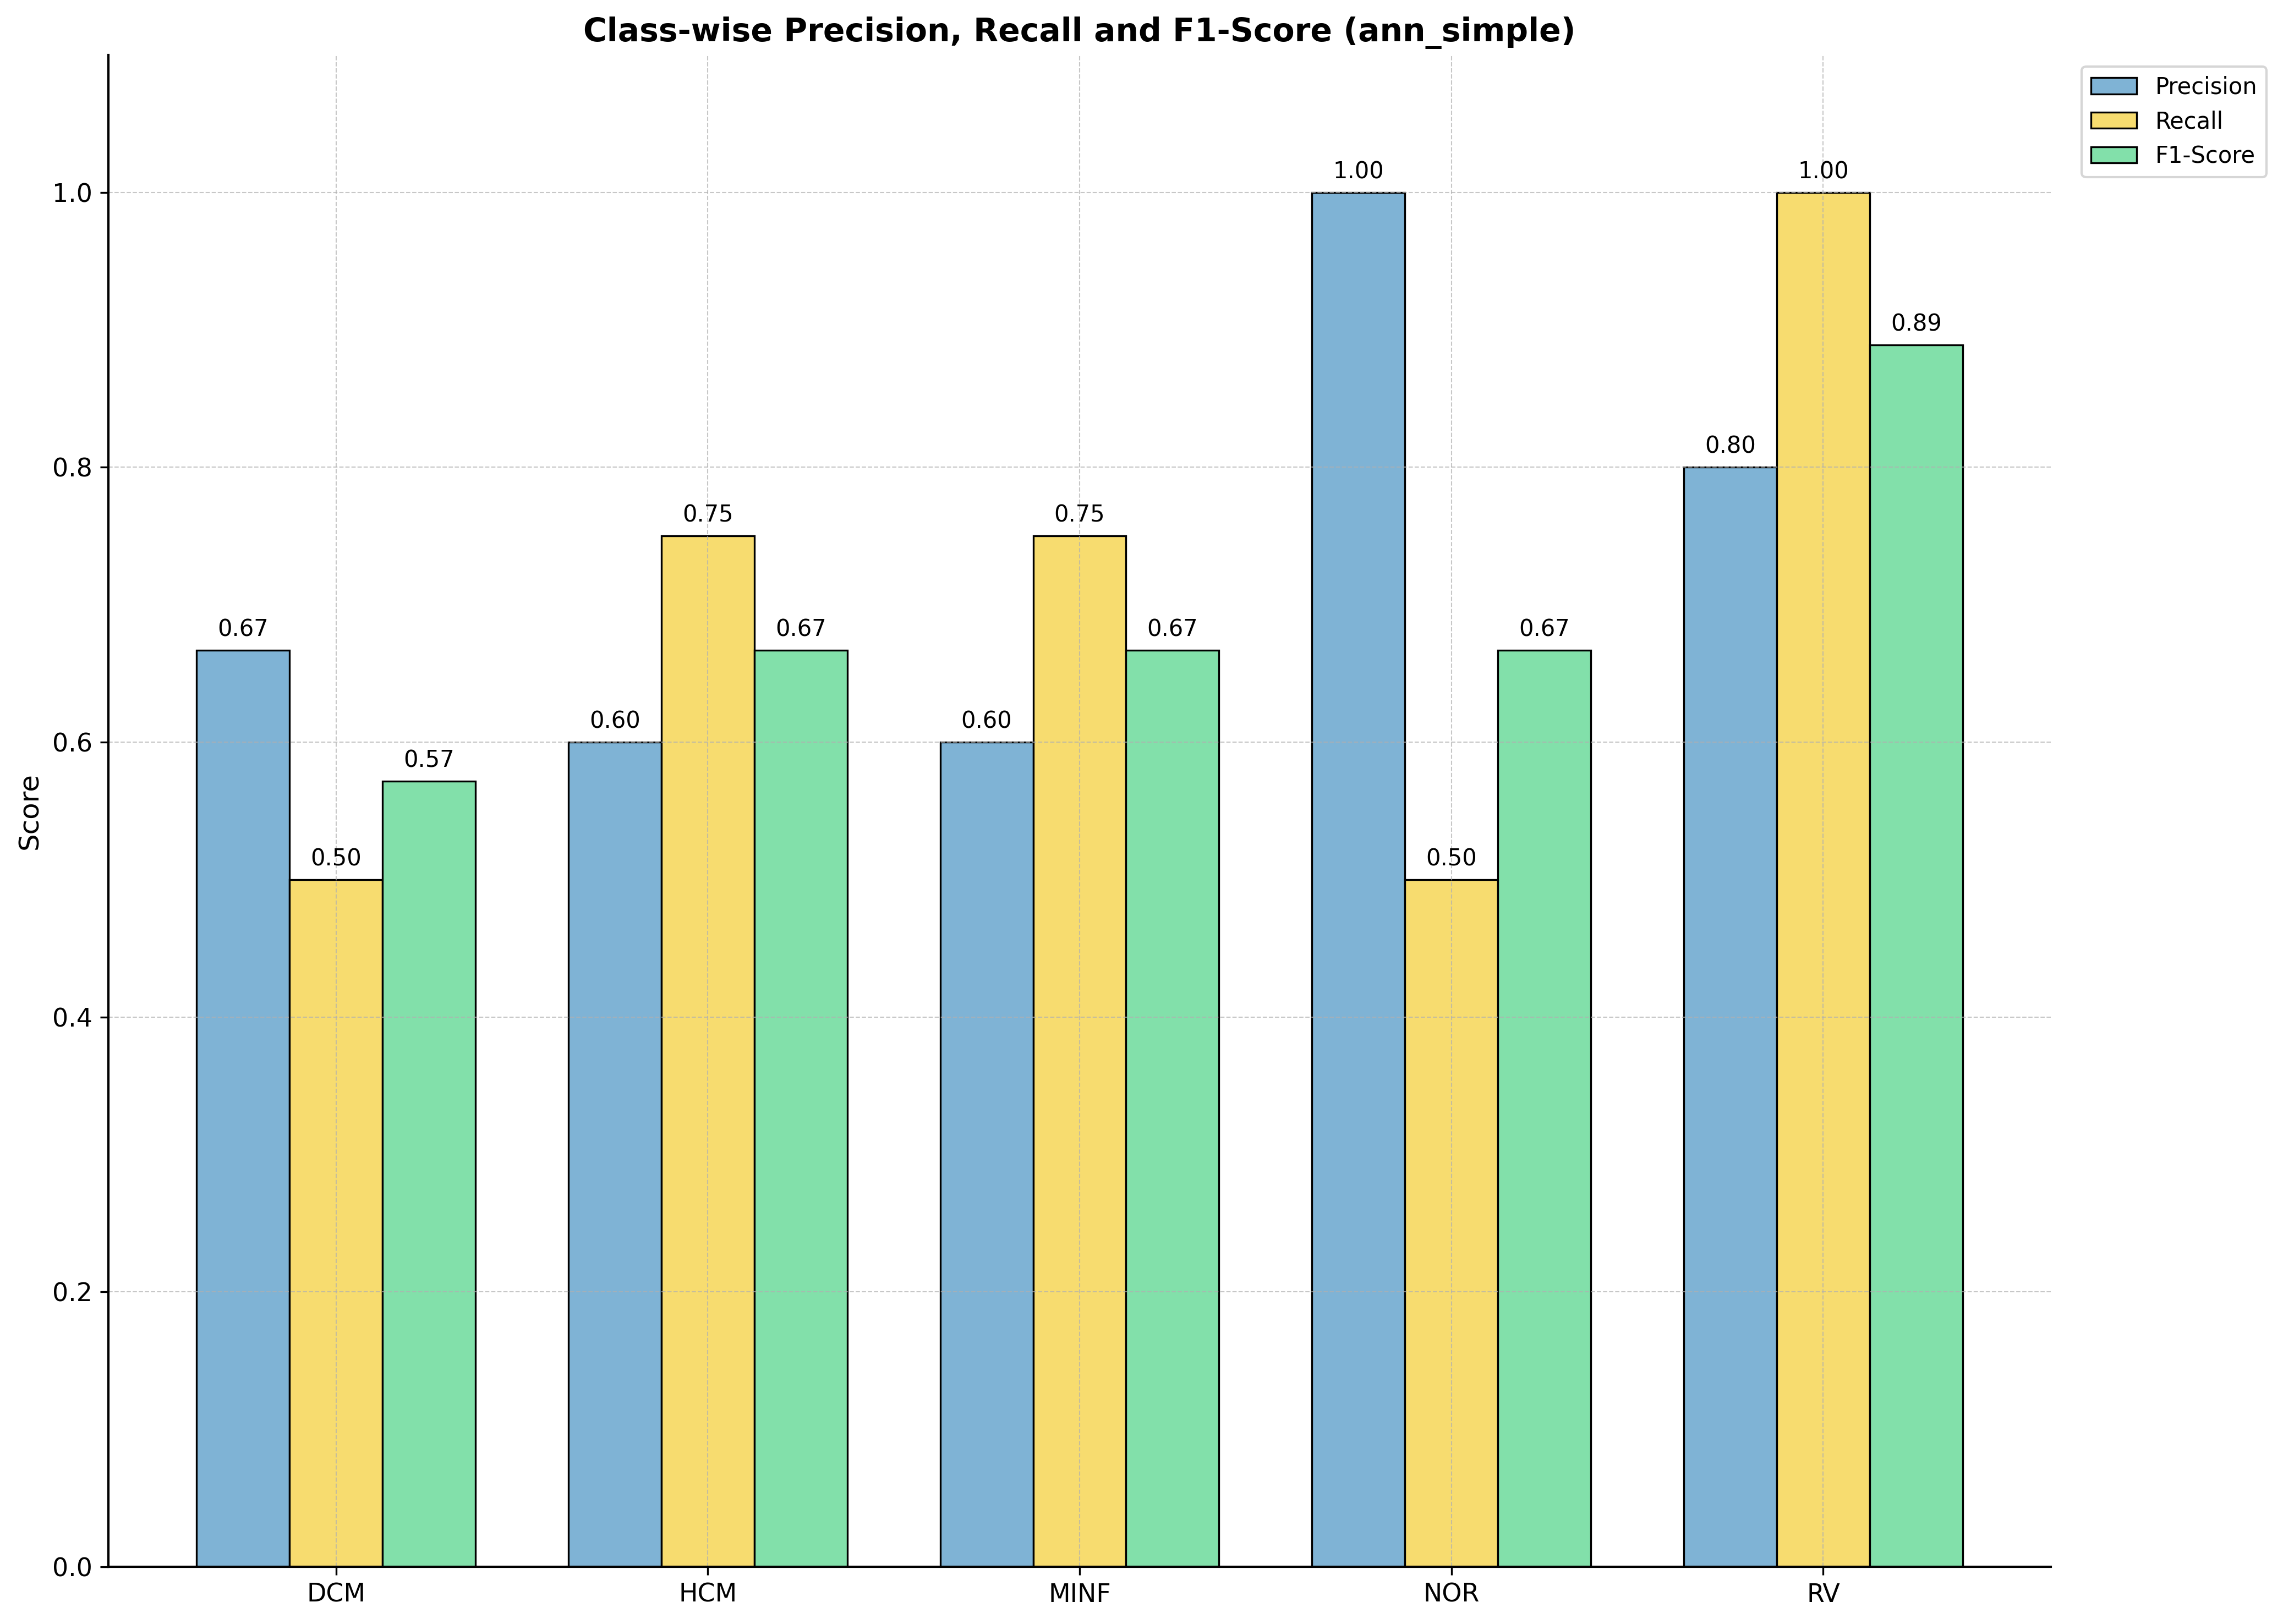
\includegraphics[width=0.85\textwidth]{../images/metrics/ann/ann_simple_class_wise_metrics.png}
	\end{center}
	\caption{Class-wise Precision, Recall, and F1-Score for the Artificial Neural
		Network (ANN) model trained using the Simple Split strategy. DCM $=$ Dilated
		Cardiomyopathy, HCM $=$ Hypertrophic Cardiomyopathy, MINF $=$ Myocardial
		Infarction, NOR $=$ Normal, RV $=$ Right Ventricular abnormality.}
\end{figure}

\begin{figure}[H]
	\begin{center}
		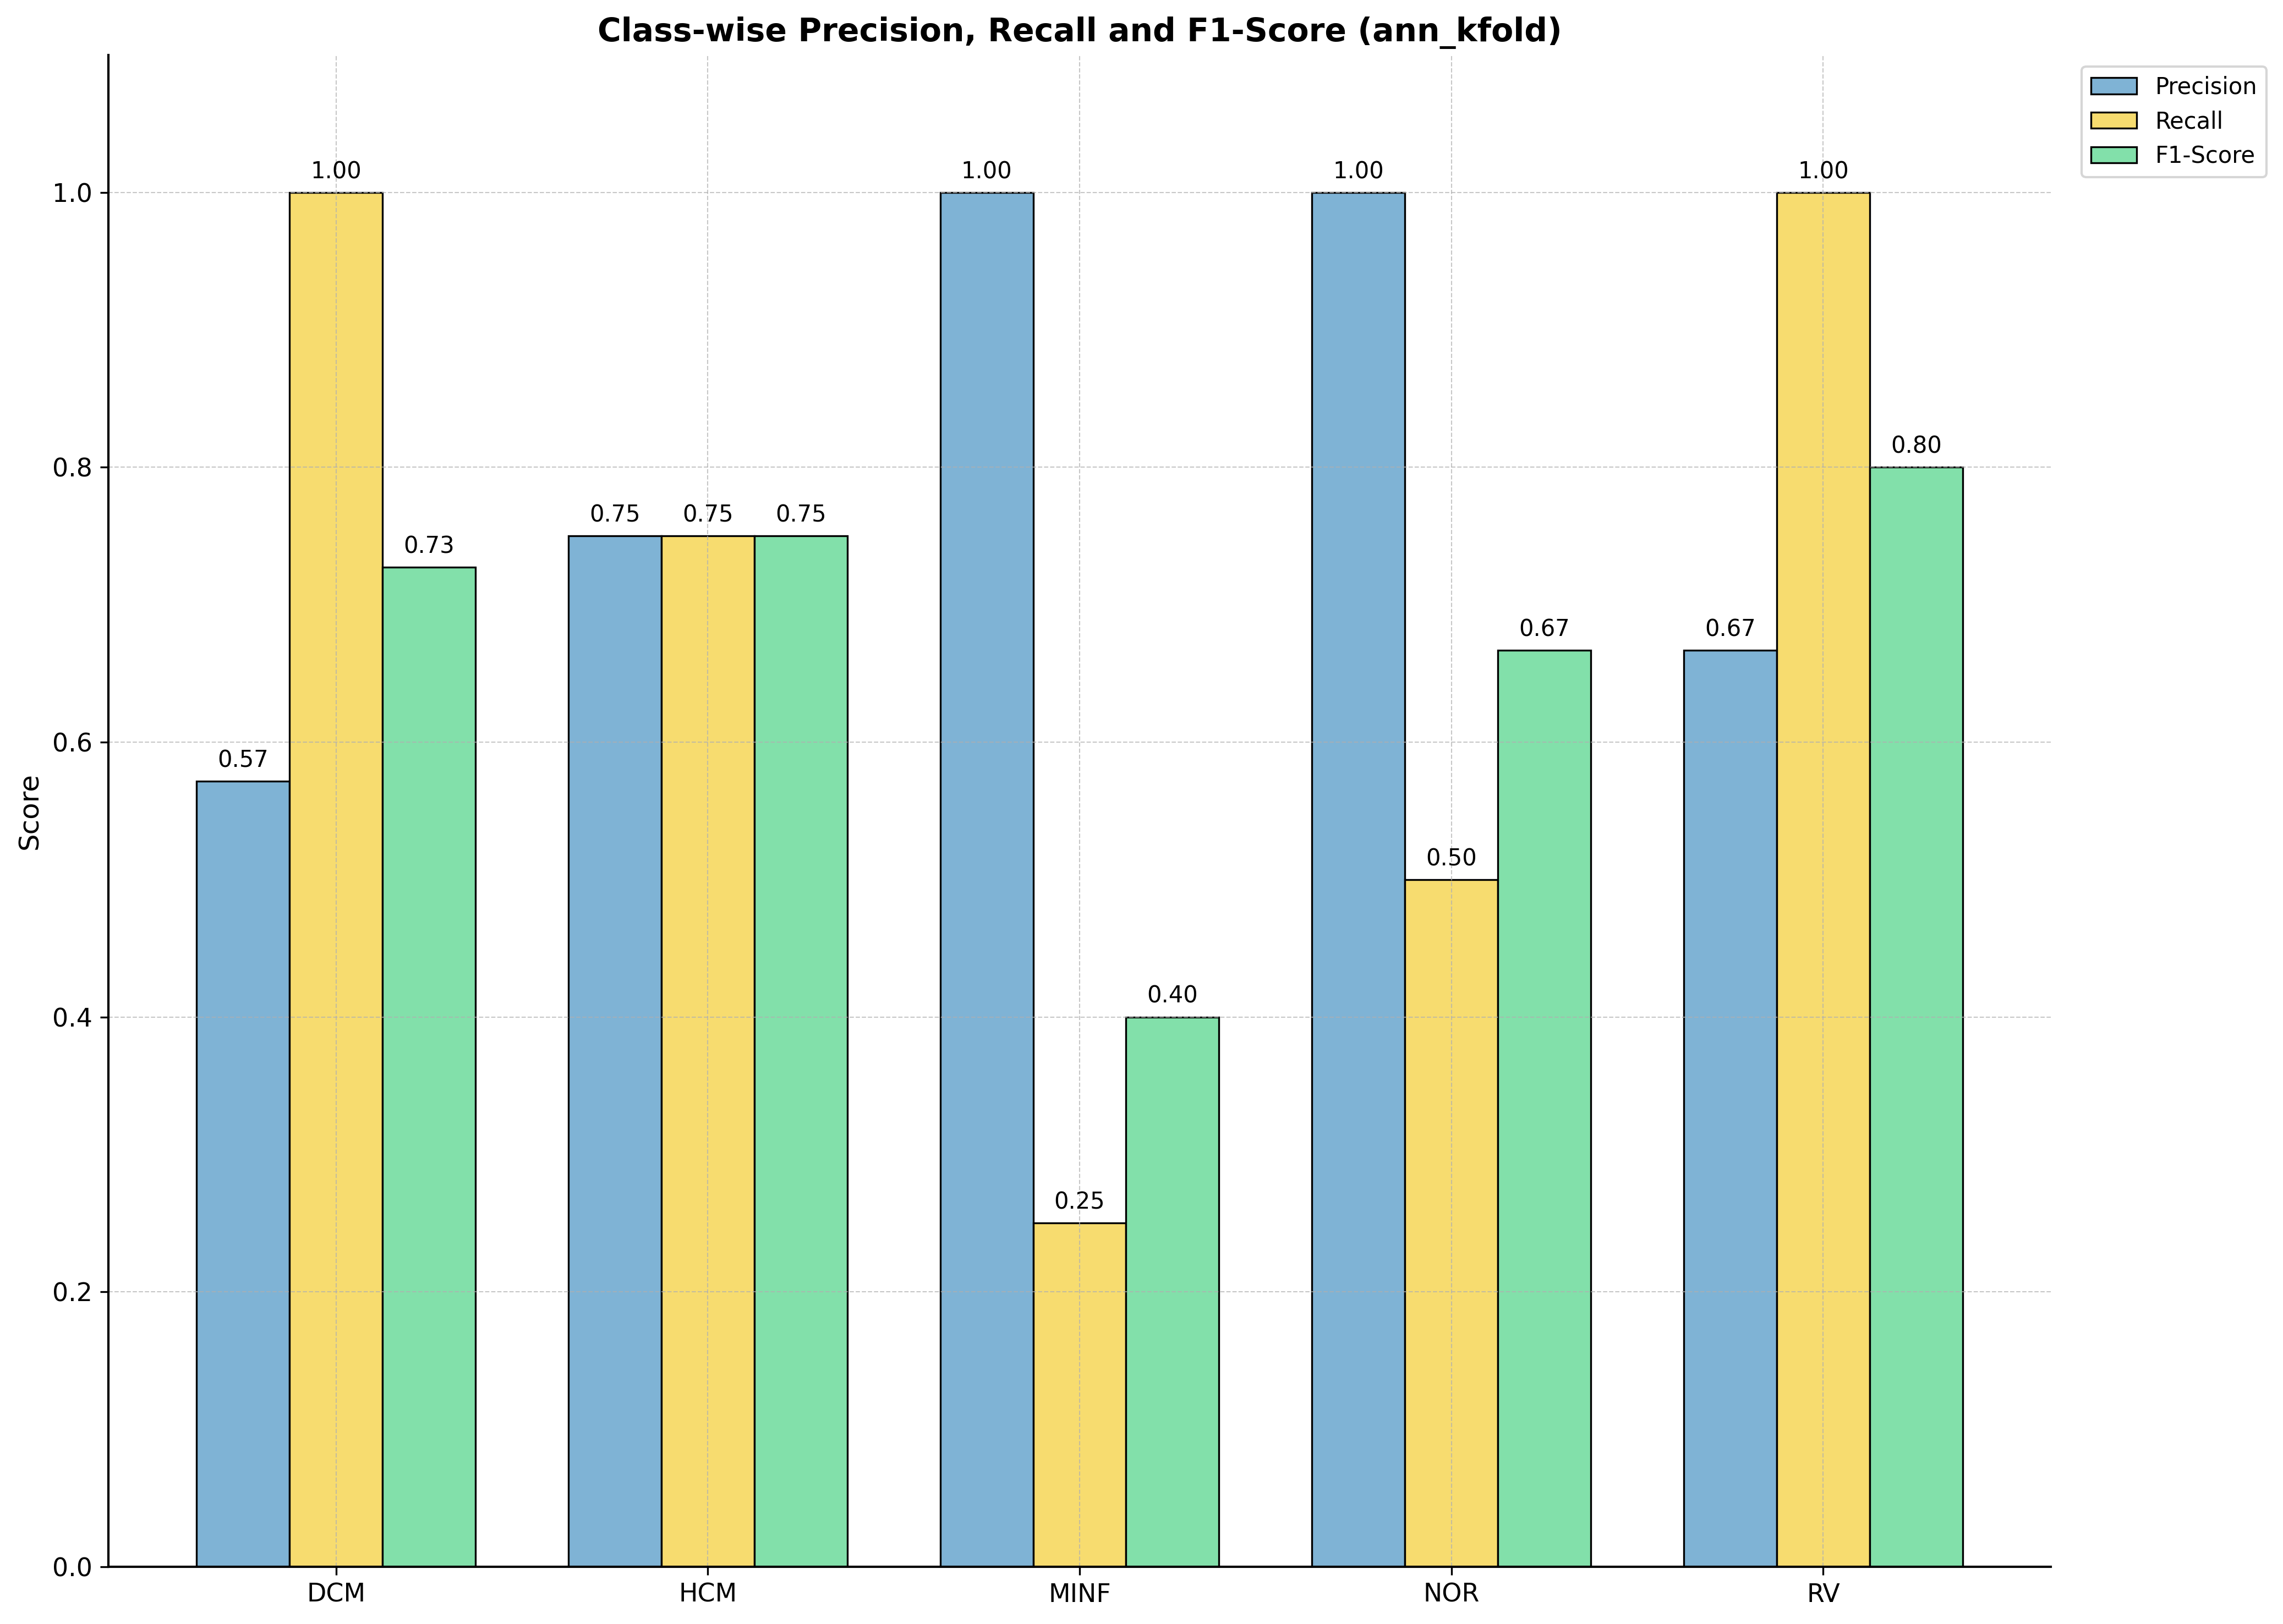
\includegraphics[width=0.85\textwidth]{../images/metrics/ann/ann_kfold_class_wise_metrics.png}
	\end{center}
	\caption{Class-wise Precision, Recall, and F1-Score for the Artificial Neural
		Network (ANN) model trained with Stratified K-Fold cross-validation. DCM $=$
		Dilated Cardiomyopathy, HCM $=$ Hypertrophic Cardiomyopathy, MINF $=$
		Myocardial Infarction, NOR $=$ Normal, RV $=$ Right Ventricular abnormality.}
\end{figure}
